%%%%%%%%%%%%%%%%%%%%%%%%%%%%%%%%%%%%%%%%%%%%%%%%%%%%%%%%%%%% 
% This is the official template for theses and seminar papers from the Chair for Information Systems for Sustainable Society (IS3) at the University of Cologne

%
%PREAMBLE
%%%%%%%%%%%%%%%%%%%%%%%%%%%%%%%%%%%%%%%%%%%%%%%%%%%%%%%%%%%%%

\documentclass[a4paper, twoside, 12pt]{article}
\usepackage[utf8]{inputenc}
\usepackage[T1]{fontenc}
\usepackage{graphicx}
\usepackage{longtable}
\usepackage{hyperref}
\usepackage{caption}

% set margins for double-sided printing \usepackage[left=2.5cm, right=2.5cm, top=2.5cm, bottom=2.5cm, bindingoffset=1.5cm, head=15pt]{geometry} \usepackage{setspace}
% set headers
\usepackage{fancyhdr}
\pagestyle{fancy}
\fancyhead{}
\fancyfoot{}
\fancyhead[LE,RO]{\textsl{\leftmark}}
\fancyhead[RE,LO]{\thesisauthor}
\fancyfoot[C]{\thepage}
\renewcommand{\headrulewidth}{0.4pt}
\renewcommand{\footrulewidth}{0pt}

\setlength{\headheight}{14.5pt} % fixes headheight warning

% set APA citation style
\usepackage{apacite}
\usepackage[numbib,notlof,notlot,nottoc]{tocbibind}
\pagenumbering{gobble}

\usepackage{amsfonts}
\usepackage{amsmath}

\usepackage{caption}
\usepackage{eurosym}
\usepackage{subcaption}
\usepackage{siunitx}

%%%%%%%%%%%%%%%%%%%%%%%%%%%%%%%%%%%%%%%%%%%%%%%%%%%%%%%%%%%%%
%THESIS Parameters 
%%%%%%%%%%%%%%%%%%%%%%%%%%%%%%%%%%%%%%%%%%%%%%%%%%%%%%%%%%%%%

\title{Extending Accessibility Analysis With True Multi-Modality}

\newcommand{\thesisdate}{January 01, 2019}
\newcommand{\thesisauthor}{Moritz Gottschling} %input name
\newcommand{\studentID}{7350270} %input student ID
\newcommand{\thesistype}{Master Thesis} % Set either to Bachelor or Master
\newcommand{\supervisor}{Univ.-Prof. Dr. Wolfgang Ketter}
\newcommand{\cosupervisor}{Philipp Peter}

%%%%%%%%%%%%%%%%%%%%%%%%%%%%%%%%%%%%%%%%%%%%%%%%%%%%%%%%%%%%%
%DOCUMENT
%%%%%%%%%%%%%%%%%%%%%%%%%%%%%%%%%%%%%%%%%%%%%%%%%%%%%%%%%%%%%

\begin{document}

%%%%%%%%%%%%%%%%%%%%%%%%%%%%%%%%%%%%%%%%%%%%%%%%%%%%%%%%%%%%%
%TITLE PAGE (Pre-defined, just change parameters above)
%%%%%%%%%%%%%%%%%%%%%%%%%%%%%%%%%%%%%%%%%%%%%%%%%%%%%%%%%%%%%
%%%%%%%%%%%%%%%%%%%%%%%%%%%%%%%%%%%%%%%%%%%%%%%%%%%%%%%%%%%%%
%TITLE PAGE
%%%%%%%%%%%%%%%%%%%%%%%%%%%%%%%%%%%%%%%%%%%%%%%%%%%%%%%%%%%%%
\makeatletter
\begin{titlepage}
    \begin{center}
        \vspace*{1cm}

        \Large
        \textbf{\@title}

        \vspace{1.0cm}
        
        \thesistype{}
        
        \vspace{1cm}

        \begin{figure}[htbp]
             \centering
             
\includegraphics[width=.5\linewidth]{./Figures/UoC_Logo.png}
        \end{figure}

        \vspace{1cm}

        \large
        \textbf{Author}: \thesisauthor{} (Student ID: \studentID{})\\
        \large
        \textbf{Supervisor}: \supervisor{}\\
        \large
        \textbf{Co-Supervisor}: \cosupervisor{}

        \vspace{1cm}
        \large
        Department of Information Systems for Sustainable Society\\
        Faculty of Management, Economics and Social Sciences\\
        University of Cologne\\

        \vspace{1cm}
        \@date

    \end{center}
\end{titlepage}
\makeatother


%%%%%%%%%%%%%%%%%%%%%%%%%%%%%%%%%%%%%%%%%%%%%%%%%%%%%%%%%%%%%
%SOOA
%%%%%%%%%%%%%%%%%%%%%%%%%%%%%%%%%%%%%%%%%%%%%%%%%%%%%%%%%%%%%
\clearpage
\thispagestyle{empty}
\section*{Eidesstattliche Versicherung}
\label{sec:SOOA}

\vspace{2.5cm}

% Statement of original authorship - Needs to be in German
% see also here: https://www.wiso.uni-koeln.de/sites/fakultaet/dokumente/PA/formulare/eidesstattliche_erklaerung.pdf

Hiermit versichere ich an Eides statt, dass ich die vorliegende Arbeit selbstständig und ohne die Benutzung anderer als der angegebenen Hilfsmittel angefertigt habe. Alle Stellen, die wörtlich oder sinngemäß aus veröffentlichten und nicht veröffentlichten Schriften entnommen wurden, sind als solche kenntlich gemacht. Die Arbeit ist in gleicher oder ähnlicher Form oder auszugsweise im Rahmen einer anderen Prüfung noch nicht vorgelegt worden. Ich versichere, dass die eingereichte elektronische Fassung der eingereichten Druckfassung vollständig entspricht.

\vspace{1cm}

\noindent
Die Strafbarkeit einer falschen eidesstattlichen Versicherung ist mir bekannt, namentlich die Strafandrohung gemäß § 156 StGB bis zu drei Jahren Freiheitsstrafe oder Geldstrafe bei vorsätzlicher Begehung der Tat bzw. gemäß § 161 Abs. 1 StGB bis zu einem Jahr Freiheitsstrafe oder Geldstrafe bei fahrlässiger Begehung.

\vspace{3cm}
\noindent
\textbf{\thesisauthor{}} 

\vspace{0.5cm}
\noindent
Köln, den xx.xx.20xx


%%%%%%%%%%%%%%%%%%%%%%%%%%%%%%%%%%%%%%%%%%%%%%%%%%%%%%%%%%%%%
%ABSTRACT
%%%%%%%%%%%%%%%%%%%%%%%%%%%%%%%%%%%%%%%%%%%%%%%%%%%%%%%%%%%%%
\clearpage
\thispagestyle{empty}
\section*{Abstract}

 [Abstract goes here (max. 1 page)]



%%%%%%%%%%%%%%%%%%%%%%%%%%%%%%%%%%%%%%%%%%%%%%%%%%%%%%%%%%%%%
%TOC,TOF,TOT
%%%%%%%%%%%%%%%%%%%%%%%%%%%%%%%%%%%%%%%%%%%%%%%%%%%%%%%%%%%%%
\clearpage
\pagenumbering{Roman}
\tableofcontents
\clearpage
\listoffigures
\clearpage
\listoftables
\clearpage

\pagenumbering{arabic}


%%%%%%%%%%%%%%%%%%%%%%%%%%%%%%%%%%%%%%%%%%%%%%%%%%%%%%%%%%%%%
%MAIN PART
%%%%%%%%%%%%%%%%%%%%%%%%%%%%%%%%%%%%%%%%%%%%%%%%%%%%%%%%%%%%%

\clearpage
\section{Introduction}
\label{sec:introduction}

%the introduction should be max. 3 pages

% --- CLIMATE CHANGE & SUSTAINABILITY ---

% more needs to be done in order to reach the goals of the Paris Agreement \cite{mitchellMyriadChallengesParis2018}.
% in order to reach the goals of the Paris Agreement emission reduction needs to start immediately \cite{krieglerPathwaysLimitingWarming2018}.
% say that it is unlikely that countries will reach the goals of the paris agreement \cite{liuCountrybasedRateEmissions2021}.
% 72\% of global transport emissions are from road vehicles \cite{Sims2014Transport}.

Climate change poses a significant threat to our planet, and reducing emissions is crucial in addressing this global challenge.
The Paris Agreement, with its ambitious goals to reduce global warming, serves as a call to action.
However, current trends suggest that without immediate action to reduce emissions, achieving these goals is unlikely \cite{krieglerPathwaysLimitingWarming2018, liuCountrybasedRateEmissions2021}.
61.8\% of global emissions in 2015 came from cities, and predictions for 2100 estimate the share to exceed 80\% by 2100 \cite{gurneyGreenhouseGasEmissions2021}.
% I need a citation that says that cities contribute majorly to global emissions
The connection between the large share of city emissions and climate change has led to a critical examination of urban planning and transportation.
In response to the urgent need to reduce emissions, the concept of emission-free cities has emerged as a pivotal strategy.
Emission-free cities aim to create sustainable environments that minimize the carbon footprint, promote the health of residents, and align with the global efforts to mitigate climate change.
Transitioning to these cities is a proactive step toward sustainable living and securing a healthier future for our urban spaces.
With vehicles on the roads accounting for 72\% of all transport-related emissions \cite{Sims2014Transport}, it is clear that urban transportation is a key area to reduce emissions.

% ---- ACCESSIBILTY-BASED PLANNING ----

In order to reduce the amount of car traffic, cities need to be planned in a way that allows people to access everything they need with alternative, more environmentally sustainable modes of transport.
Therefore, a recent trend in urban planning is accessibility-based planning \cite{proffittAccessibilityPlanningAmerican2019} \cite{geursAccessibilityEvaluationLanduse2004a}.
% ---- ACCESSIBILTY METRICS ----
In order for practitioners to be able to plan cities in an accessibility-based way, they need to be able to measure accessibility.

% ---- 15 MINUTE CITIES ---- into multi modal & needs for our tool
A modern way of measuring accessibility is to use the X-minute city metric, which is inspired by the 15-minute city concept, which recently gained traction during the COVID pandemic \cite{morenoIntroducing15MinuteCity2021}.
The concept of the 15-minute city is that all the things a person needs to live a good life should be accessible within 15 minutes of walking or cycling.
Traditionally, the modes of transport don't include public transportation or vehicle sharing systems.
However, we argue that in order fully grasp the potential of sustainable transport, it's essential to incorporate all modes, not merely a subset, in the measurement of accessibility.
We therefore develop a new method for accessibility-based planning that incorporates all modes of travel (multi-modal, unrestricted inter-modal).
In addition, this method will incorporate a metric based on the concept of the 15-minute city, extending it to include all modes of transport and therefore presenting a more holistic view on accessibility via sustainable modes of transport.
Finally, we apply our method on the City of Cologne.

% multi-objective & equality stuff is kind of missing
%- (hopefully) give recommendations to practitioners on how to enable equal & fair accessibility (multi-objective)

The remainder of this paper is structured as follows.
In Section \ref{sec:related_work}, we present related work on accessibility-based planning, the 15-minute city concept, and routing algorithms.
Next, in Section \ref{sec:method}, we describe the specifics of our method, including the data collection process, the routing algorithm, and the accessibility metric.
After that, we introduce the case example, we will apply our method on in Section \ref{sec:experiment} and present the results in Section \ref{sec:results}.
Finally, we conclude with our discussion Section \ref{sec:discussion}.


\clearpage
\section{Related Work}
\label{sec:related_work}

...

\subsection{Accessibility Analysis}
\label{subsec:accessibility_analysis}


...
In order to assess the accessibility from a given origin to one or multiple
points of interest, a routing algorithm is required. The routing algorithm finds
the shortest path from the origin to the destination.

\subsection{Routing Algorithms}
\label{subsec:routing_algorithms}


\subsubsection{Dijkstra}
\label{subsubsec:dijkstra}
The most straightforward approach to compute the shortest paths in a graph is
the Dijkstra algorithm \cite{dijkstra1959note}. The Dijkstra algorithm operates
on a graph \( G = (V, E) \), where \( V \) is the set of nodes and \( E \) is
the set of edges. Each edge \( e \in E \) has a weight
\( w(e) \in \mathbb{R}\). The graph data structure is general enough to
represent a wide range of problems, including road networks and public
transport networks.

Dijkstra's algorithm initiates at a designated start node \( s \in V \) and
employs a priority queue to systematically determine the shortest path to each
subsequent node \( v \in V \). Initially, the distance to the start node \( s
\) is set to zero, while the distances to all other nodes are set to infinity.
In each iteration, the algorithm dequeues the node \( u \) with the smallest
known distance from the priority queue. It then examines each outgoing edge \(
e = (u, v) \) from \( u \), updating the distance to \( v \) if a shorter path
through \( u \) is discovered. Specifically, if
\( \text{dist}(u) + w(e) < \text{dist}(v) \), then \( \text{dist}(v) \) is
updated to \( \text{dist}(u) + w(e) \), and \( v \) is enqueued into the
priority queue for future exploration. The node \( u \) is marked as visited by
adding it to the set \( V_{\text{visited}} \).

However, this simple approach has multiple problems. Firstly, the Dijkstra
algorithm is not able to handle multiple criteria. Secondly, the runtime of
Dijkstra's algorithm is \( O(|E| + |V| \log |V|) \), which is too slow for
large graphs.

\subsubsection{MLC}
\label{subsubsec:mlc}

The Multi-Label Correcting (MLC) \shortcite{hansenBicriterionPathProblems1980}
extends Dijkstra's algorithm to handle multiple criteria. Concerning the inputs,
the only difference between Dijkstra's algorithm and MLC is that the edges in
the graph has vectors as weights instead of scalars \( w(e) \in \mathbb{R}^k \).




One of the most prominent routing algorithms for public transport is the Round
based Public Transit Optimized Router algorithm (RAPTOR)
\cite{dellingRoundBasedPublicTransit2015}, which is also used by R5. The RAPTOR
algorithm (Round-Based Public Transit Optimized Router) is designed to compute
all Pareto-optimal journeys in a dynamic public transit network. Unlike
traditional Dijkstra-based algorithms, RAPTOR operates in rounds, looking at
each route (such as a bus line) in the network at most once per round. This
makes it highly efficient and capable of handling fully dynamic scenarios,
including delays and cancellations.
In order to allow intermediate transfers between trips, e.g. walking between
stops, RAPTOR uses a transitively closed transfer graph. More precisely RAPTOR
takes a graph as an input whose nodes are stops and whose edges represent
transfers without a schedule, meaning that the transfer can be made at any time.
The original RAPTOR papers suggests no method to compute the transfer graph.
Theoretically, this graph is enough to constitute all possible journeys.
However, in practice, it can be very challenging to compute the graph and it
can be very large.

To overcome problem of RAPTOR \cite{dellingComputingMultimodalJourneys2013}
introduce Multimodal Multicriteria RAPTOR (MCR). MC

ULTRA

\clearpage
\section{Method}
\label{sec:method}

% Initially, we establish a metric based on the concept of the 15-minute city, by evaluating the existing metrics introduced in Section \ref{subsec:accessibility_metrics_based_on_the_15_minute_city} and their shortcomings and then developing our own metric that overcomes these limitations.
Our method is split into three parts.
Initially, we establish a metric based on the concept of the 15-minute city and complement it with a cost metric.
Following this, our focus shifts to finding a fitting routing algorithm to calculate this metric.
We do so by clearly stating the requirements we pose on such an algorithm, explaining why existing algorithms don't meet our criteria, and introducing our own algorithm, designed to meet our requirements. 
The final stage explains how we use our routing algorithm to calculate our metric. 
This integrated approach allows us to thoroughly assess and improve accessibility in urban settings, offering valuable insights for urban planners and decision-makers.

\subsection{Metric}
\label{subsec:metric}

Our metric consists of two dimensions, time and cost.
The time dimension is based on the concept of the 15-minute city and expands on the findings of \shortciteA{olivariAreItalianCities2023}.
The time dimension effectively measures how fast the access to a variety of important amenities is.
To measure this, we categorize amenities into seven essential services: grocery, education, health, banks, parks, sustenance, and shops.
Each category is populated with Points of Interest (POIs) sourced from OSM, providing a comprehensive database of locations.
The POIs are identified by their respective OSM tags.
OSM tags are descriptive labels used to define the attributes and characteristics of geographic features in the OSM database. 
They consist of a key and a value pair, like "amenity=restaurant", which enables categorizing map elements such as roads, buildings, and natural features for accurate and comprehensive mapping.
In our case, we use the OSM tags to identify nodes that represent POIs, like a supermarket or a park.
The categories and their respective tags can be seen in Appendix \ref{app:categories_and_osm_tags}.

The core of our metric is the determination of temporal proximity to these amenities. 
For each category, we calculate the minimum travel time required to reach at least one POI of that category. 
The metric is then defined as the maximum value among these minimal times across all categories and we refer to it as the X-minute city metric, where X represents the maximum value among the minimum travel times.
This approach yields a singular measure that reflects the most significant time distance barrier within an urban area, which effectively captures the least accessible category for any given area.
We think that it is beneficial to focus on the least accessible category, as measuring accessibility in cities by averaging accessibility across all categories can mask disparities categories. 
This ensures that the metric is targeted to areas of greatest need. 
By leveraging this metric, we aim to help city planners to create urban environments that prioritize sustainability, enhance the well-being of residents, and reduce dependency on vehicular transport, thus contributing to the broader goals of efficient urban planning and improved quality of urban life.

% --- comparison to NEXI
Our metric presents several advantages compared to the NEXI-minutes and NEXI-global, as outlined by \shortciteA{olivariAreItalianCities2023}.
Firstly, unlike the NEXI-minutes which calculates separate metrics for each of seven categories, our metric evaluates all categories together. 
This unified approach makes it more straightforward and easier to understand. 
In contrast, while NEXI-global also considers all categories in one assessment, it converts the results into a 0-100 score. 
This percentage system can obscure the real value of the data, making it more difficult to interpret.

Moreover, the NEXI-global's practice of assigning different weights to each category complicates its analysis. 
Our metric, by focusing on the lowest-performing category across all areas, simplifies the understanding and highlights where improvement is most needed. 
This method prevents the dominance of stronger areas over weaker ones, ensuring a more balanced and fair evaluation of urban development. 

% --- cost
In addition to the time dimension, we also incorporate a cost dimension into our metric.
As, we want to incorporate more modes than just walking, some of which may have a monetary cost associated with them, we need to consider the cost of the trip.
We recognize that time and cost are measures of different units and cannot be combined in a sensible way.
Therefore, we draw upon the notion of Pareto optimality to create a multi-objective metric that considers both time and cost.
We define a Pareto set as a set of tuples, where each tuple contains a time value and a cost value.
A tuple can be considered the time that is needed to reach all categories given the cost value.
The Pareto set will allow answering questions in the form of "What is fastest time I can reach all categories given a certain cost?" or "What is the lowest cost I need to pay to reach all categories given a certain time?".

% ---- START section about alternative modes
% explain different modes - maybe(?) this belongs to related work
Traditionally, the 15-minute city concept is applied to walking and or cycling and ignores other modes of transport.
Some researchers, in the context of location-based metrics, even go as far to only calculate the bee-line distance to the nearest amenity and ignore the street network altogether \shortcite{gastnerOptimalDesignSpatial2006}, while most only consider walking \shortcite{olivariAreItalianCities2023, nicolettiDisadvantagedCommunitiesHave2023}.
We, however, believe that to accurately determine the accessibility of a city, all modes of transport must be considered, and the routing needs to be as realistic as possible.
Therefore, we continue with the discussion of requirements we pose on our routing algorithm next.


\subsection{Routing Algorithm}
\label{subs:routing_algorithm}

In this section we will first define the requirements we pose on our routing algorithm and explain why existing algorithms don't meet our criteria.
Next, we will explain our algorithm in detail, which is based on a modular approach, where one module represents one mode of transport.
After that we will explain the modules we use in our experiments, which are either based on MLC or McRAPTOR.
Lastly, we will explain some enhancements we made to MLC and McRAPTOR in order to support multi-objective optimization with dynamic pricing schemes.

\subsubsection{Requirements}
\label{subsubsec:requirements}

% requirements on routing algorithm
% - unrestricted
% - multi-modal (must incorporate scheduled networks (public transfer) and an arbitrary number of other unscheduled networks)
% - multi-objective (must be able to incorporate an arbitrary amount of objectives), whose values update based on the previous values and the current edge (either unscheduled network edge or trip between two stops)
% - inter-modal (the different transport modes may be sequenced in any order (not just bicycles for start and end)
% - modular (the algorithm should be easily adaptable to different modes of transport and the combination of different modes of transport)

In order to fully grasp the potential of the combination of the sustainable modes of transport, we require our routing algorithm to be \textbf{multi-modal}, \textbf{multi-objective}, \textbf{unrestricted inter-modal}, and \textbf{modular}.

\textbf{Multi-modal} means that our routing algorithms allows multiple modes of transport, including scheduled transport systems, like public transfer and an arbitrary number of unscheduled transport systems, like walking, cycling and driving.
In addition, we require that free-floating vehicle sharing systems are incorporated realistically.
That means, that our routing algorithm must consider that switching to a free-floating vehicle is possible at any location, where a free-floating vehicle is available and parking a free-floating vehicle is possible anywhere where it's allowed.
% note: this extra excludes MCR

\textbf{Multi-objective} means that our algorithm must find all pareto optimal journeys according to an arbitrary amount of objectives.
The algorithm must provide the possibility to update the values of any objective whenever a \textit{movement} occurs.
We define a movement either as an edge traversal in an unscheduled network or a step in the route traversal during McRAPTOR.
In the case of an edge traversal the new objective must be a function of the old objective and the edge weights, formally: \(l' = f(l, w(e))\), where \(l\) and \(l'\) are the old and new labels, respectively, and \(w(e)\) are the weights of the edge that is traversed.
In the case of an update during a step of the route traversal, the new objective must be a function of the old objective (to be continued).

\textbf{Inter-modal} means that the different transport modes may be sequenced in any order.
For example, when considering walking, cycling through a bicycle sharing system and public transport, the algorithm needs to consider journeys with bicycle rides between two consecutive public transport trips.

\textbf{Unrestricted} means that the algorithm fully searches the unscheduled network graphs, and does not pose restrictions like a maximum of 10 minutes walking distance.

\textbf{Modular} means that the algorithm should be easily adaptable to different modes of transport.
It should be possible to easily add, remove or chain different modes of transport.


% handled:
% dijkstra, mlc, raptor, ultra, mcraptor, mcr
% relate to other algorithms
Both Dijkstra and MLC are not considered due to their impractical runtime.
Furthermore, the need for multi-objective solutions excludes Dijkstra, RAPTOR, and ULTRA.
The requirement for unrestricted inter-modal travel makes RAPTOR and McRAPTOR unsuitable in practical scenarios.
To explain this, let's examine a straightforward example.
Consider the OSM graph of the key regions in Cologne, which comprises 125,176 nodes and 142,074 edges.
For RAPTOR to compute a transitively closed graph, it requires calculating the walking distance between each node.
This computation would yield \(125,176^2 = 15,669,030,976\) edges, a number vastly greater than the original 142,074 edges.
While MCR does support multi-objective solutions with unrestricted inter-modal transfers, it doesn't fully encapsulate the multi-modal concept we require.
Although it theoretically permits various modes of unscheduled transport, it is primarily tailored for station-based vehicle sharing systems.
Our focus, however, is on the increasingly prevalent free-floating systems.
In MCR, unscheduled networks are contracted, leading to the removal of certain nodes.
If an optimal route requires a mode change at a deleted node, MCR will be unable to identify that path.
As a result, MCR is not a viable option for our needs.
Also note, that none of the algorithms mentioned so far are modular.

\subsubsection{Scaffolding Algorithm}
\label{subsubsec:algorithm}

% introduction modules
As said, our algorithm should be easily adaptable to different modes of transport, therefore, we formulate it in a modular fashion.
The algorithm described next presents a scaffolding that needs to be augmented by different modules, where a module represents a specific mode of transport and running a module may be seen as fully exploring the network through this mode of transport.
One module, for example, would be walking, and running the walking module would mean to traverse the whole walking graph given the current state of bags.

% explanation of bags & need for common network 
A module always takes bags as an input and returns bags as an output.
As explained in Section \ref{sec:related_work} a bag is a set of labels, that are Pareto optimal with respect to the objectives.
In addition, in our work, a bag is associated with a node on some network.
For the bags that are the input and output of the modules, we further require that they are associated with the same network.
This is necessary in order to merge the bags of different modules.
The most reasonable choice for the common network is the walking graph, as this has a real-world interpretation, because walking between different modes of transport is very common.

% example of running a module
To further explain how running a module looks like, consider the example of calling the walking module on the starting bags, which are a set of bags, where every bag is empty, except for the one of the starting node, where exactly one label is present that contains the starting time and zero costs.
The output would be a set of bags, where each node's bag contains exactly one label where the time would be equal to the time it takes to walk to the node and the cost would be zero, as walking never costs anything.

% algorithm
The scaffolding algorithm is shown in Figure \ref{fig:modular_routing_algorithm}.
The algorithm takes a start node and time as input and returns bags.
First it creates the starting bags described above from the start node and the start time.
Next, it runs the initial modules given by the initial module matrix.

A module matrix is an irregular matrix of modules.
To run the module matrix, first the modules of the first row are run in parallel.
Their respective outputs are then merged into a single set of bags.
After that the second row is run and so on and so forth.
This process is also described in Figure \ref{fig:modular_routing_algorithm}.

After the initial modules are run, the same is done for the repeating modules for the specified number of times.
By convention, we count each iteration of the repeating modules as one trip.

\begin{figure}
    \centering
    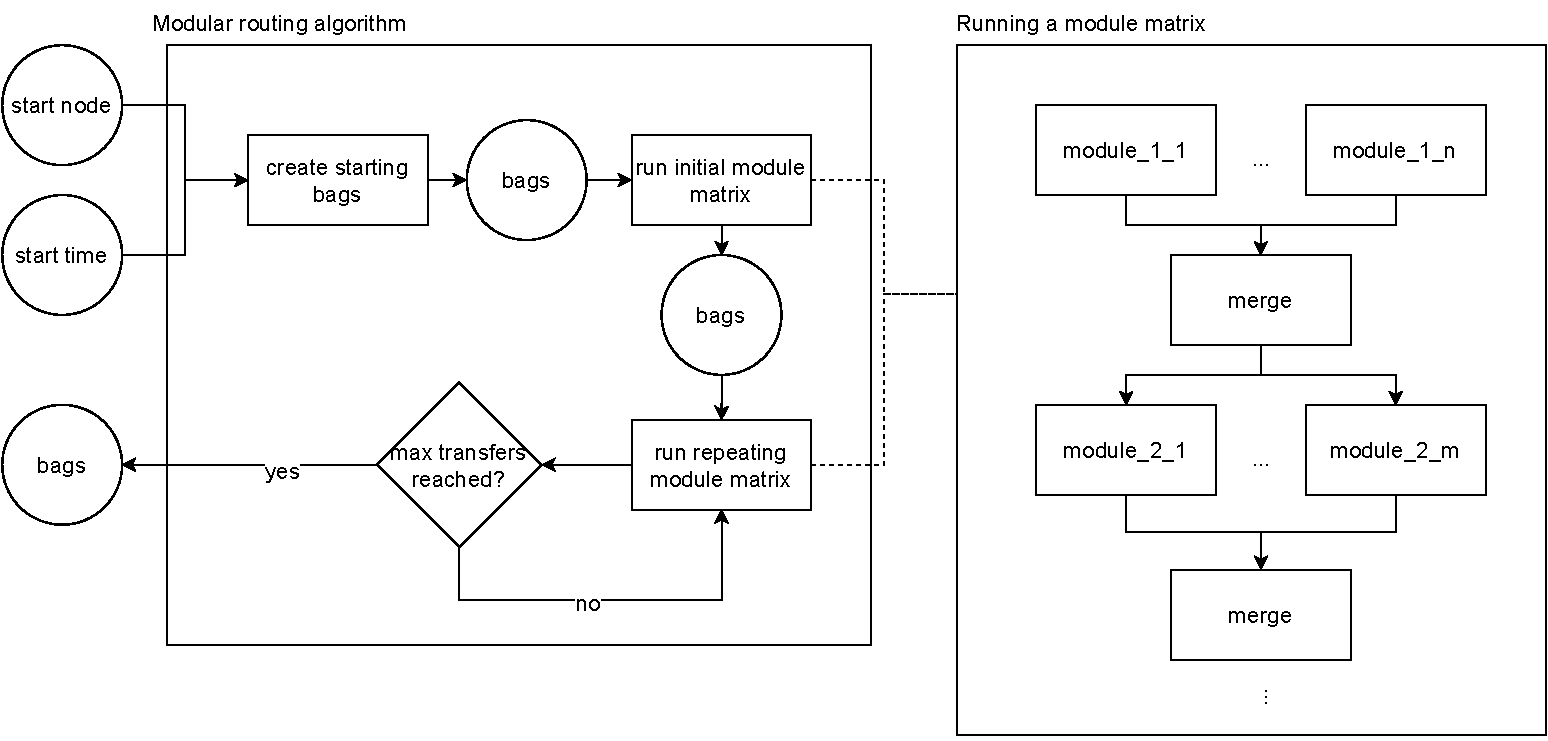
\includegraphics[scale=0.40]{Figures/method/modular_routing_algorithm}
    \caption{Modular Routing Algorithm}
    \label{fig:modular_routing_algorithm}
\end{figure}


\subsubsection{Modules}
\label{subsubsec:modules}

In our experiments, we categorize four modules into two types: unscheduled and scheduled. 
The unscheduled modules consist of walking, free-floating vehicle sharing, and personal vehicle use and are based on MLC, while the scheduled module is public transport, which is based on McRAPTOR.

Walking is the simplest unscheduled module, it simply consists of running MLC on the walking graph.
The edges of the walking graph should contain the time it takes to traverse them by foot and should not have any monetary cost associated with them.

The free-floating vehicle sharing module is a bit more complex.
Before running MLC on the respective vehicle graph, the module filters our all bags that are located at a node where no free-floating vehicle is available.
In addition, the vehicle graph is augmented with a walking graph. 
This means that at nodes in the vehicle graph, where it is allowed to park the vehicle, there is an edge to the closest node in the walking graph.
This augmentation is necessary, as the output bags of the free-floating vehicle sharing module need to be associated with nodes in the walking graph, as it is the common network.
The module may also define any form of monetary cost.

For the personal vehicle module, we assume that there is only one personal vehicle and that it is located at the starting node.
Therefore, the module filters out all bags that are not located at the starting node.
Obviously, this module is only useful for the first trip, or more precisely, the module should only be used in the first row of the initial module matrix.
After that MLC is run on the vehicle graph again augmented with the walking graph.
% TODO: monetary cost

In comparison to the unscheduled modules, the public transport module does not use MLC, but McRAPTOR.
As a first step the module filters out all bags that are associated with a node that is not near a stop in the public transport system.
Next, the module performs a single iteration of McRAPTOR, which represents a single trip within the public transport system.
Last, the resulting bags have to be associated with nodes in the walking network again.
To do so, the modules simply use the node that is closest to the coordinates of the public transport stop.
Just like the free-floating vehicle module, the public transport module may define any form of monetary cost.

\subsubsection{Merging}
\label{subsubsec:merging}

The merging of bags after running multiple modules in parallel is quite simply.
Each bag represents a set of Pareto optimal labels and each bag is associated with a node.
We therefore merge bag-wise.
We differentiate between two cases:
\begin{enumerate}
    \item There is only one bag associated with a node.
    \item There are multiple bags associated with the same node.
\end{enumerate}
In the first case, we simply put the bag into the output bags.
In the second case, we create a new bag that contains all labels of all bags associated with the node, which might break the Pareto optimality of the labels.
Therefore, to restore the Pareto optimality of the labels, we remove all labels that are dominated by another label.

\subsubsection{Enhanced MLC \& McRAPTOR}
\label{subsubsec:enhanced_mlc_and_mcraptor}

To address the multi-objective optimization involving both time and monetary cost, we introduce enhancements to MLC and McRAPTOR. 
The standard versions of MLC and McRAPTOR do not adequately capture dynamic pricing models, which is necessary to realistically represent monetary costs.

% \paragraph{Challenges in the Original Algorithms} 
The original MLC associates a fixed cost with an edge, which cannot represent variable pricing, such as a bike-sharing tariff that costs 1euro per 15-minute increment. 
Labels are only updated by adding the cost of a given edge to the label's values.
Similarly, McRAPTOR updates the labels at each stop during route traversal only based on the information of the current trip and stop. 
With this McRAPTOR is unable to represent a pricing scheme that varies with the number of stops, like the one used by the Cologne Transport Authority.
Our proposed modifications involve the use of 'hidden values' within the labels that are used by these algorithms. 
These hidden values carry additional information which is not considered when comparing labels, but that may be used to update cost dynamically.

In the case of MLC, the hidden values may be updated along any edge, just like the regular values of the label.
A hidden value, may carry information on how long the current trip with the shared vehicle is.
We then additionally allow defining a function that updates while traversing an edge and may use the values and hidden values both before and after the traversal to do the update.
With this functionality it is easy to increment the cost by 1euro every time the time spent on the trip exceeds the 15-minute interval.

Similarly, the hidden values may be updated during McRAPTOR after every iteration of a stop.
We can, therefore, store how many stops the current trip already traversed and if that number exceeds four, we can easily increase the price from 2.20euro to 3.20euro.

Additionally, as the concept of hidden values isn't specific to MLC or McRAPTOR, the hidden values can be transferred across iterations and modules.
To understand the benefit, again consider the example of the pricing of the Cologne Transport Authority.
The ticket that costs 3.20euro allows traveling any number of trips within Cologne, no matter if it is necessary to change to a different trip.
Therefore, if we were to first travel two stations with one trip and then get out to catch another trip that consists of five stops, we would still have the information that we already commuted two stops.
Therefore, we can charge 3.20euro, instead of charging 2.20euro two times, which is more realistic.
These enhanced versions of MLC and McRAPTOR are used in our modules, so that we can use the more realistic dynamic pricing schemes.

While running our experiment, we see that MLC based modules present a significant computational bottleneck.
We observe that in order to calculate our metric, we don't actually need to have the labels of every single node, but only of those, that impact the X-minute city and time Pareto front.
We therefore introduce a runtime optimization into MLC, which eliminates some bags from being processed that are guaranteed to not impact the Pareto front.
While iterating the unprocessed bags in MLC, we keep track of the minimum time required to reach a POI node of each category for each cost value.
If we encounter a bag whose time and cost values are both greater than the minimum time and cost values for all categories, we can safely discard this bag, as it will not impact the Pareto front.


\subsubsection{Example}
\label{subsubsec:example}

To illustrate our algorithm, we will now go through an example step by step.
The module configuration we use in our example represents travelling by free-floating vehicle sharing, public transport and walking.
The initial module matrix just contains the walking module, in order to initially reach the free-floating vehicles, as well as, the public transport stops.
The repeating module matrix consists of first the free-floating vehicle sharing module and the public transport module in parallel and then the walking module.
It can be seen in Figure \ref{fig:example_module_matrix}.


\begin{figure}[ht]
\centering
\[
\begin{pmatrix}
\text{free-floating vehicle} & \text{public transport} \\
\text{sharing module} & \text{module} \\
\\
\text{walking} & \\
\end{pmatrix}
\]
\caption{Example Repeating Module Matrix}
\label{fig:example_module_matrix}
\end{figure}

In our example, we assume that both public transport and vehicle sharing has some form of cost associated with it.
The objective is to minimize arrival time and cost.
We also only consider a maximum of two trips.

First we run the initial modules, which in our case is just the walking module on the starting bags.
As the starting bags only consist of one non-empty bag at the starting node with exactly one label, running MLC on the walking graph is equivalent to running Dijkstra's algorithm.
In the real-world this represents walking to all nodes in the walking network from the start node.
Note, that after the initial walking module all bags only contain exactly one label, as the cost to go anywhere by foot is zero.

Next the modules of the first row of the repeating matrix are run.
In the real-world this means that after an initial walk the traveler would either drive with a free-floating vehicle starting from a location where one is available or commute by public transport starting from one stop.
For public transport one could imagine that we commute with all possible trips from all stops and update the bags of the stops along each route accordingly.
After running these modules and merging their result bags, each bag may contain more than one label, as public transport and driving with a vehicle may be faster than walking, but also cost money.
It may even be that some bags contain three different labels, if, for example, driving with a vehicle is the fastest but also costs the most money and commuting by public transport is faster than walking.
The next step consists of running the second row of the repeating module matrix, which in our case is the walking module again.
Running the walking module in the repeating module matrix is important in order to reach nearby POIs after commuting through the public transport system.
After that the repeating module matrix is run again, as we consider a maximum of two trips.
The result of the second run of the repeating module matrix is our final result.



\subsection{Integrated Accessibility Analysis Routine}
\label{subsec:combining}

We embed the routing algorithm described in Section \ref{subsec:routing_algorithms} in our accessibility analysis routine to compute the metric described in Section \ref{subsec:metric}.
Our accessibility analysis routine consists of three parts: the input routine, the main routine and the metrics routine.

% Input routine
\begin{figure}
    \centering
    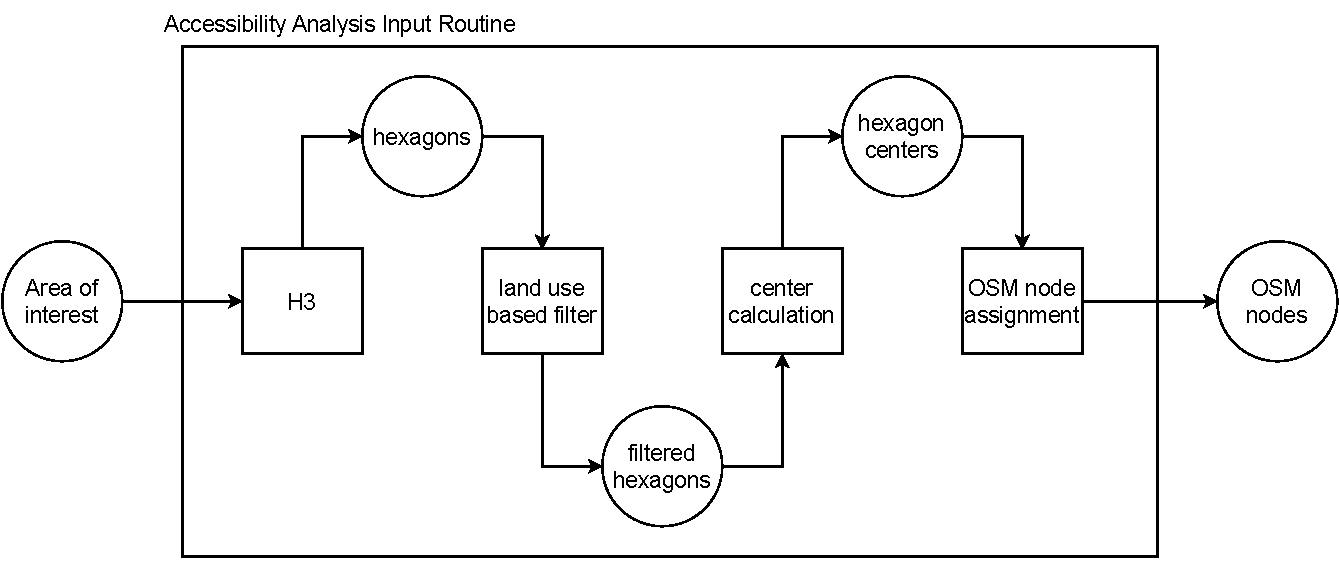
\includegraphics[scale=0.60]{Figures/method/input_routine}
    \caption{Input Routine}
    \label{fig:input_routine}
\end{figure}
In the input routine, depicted in Figure \ref{fig:input_routine}, we first create an even grid that covers the whole area of interest, for example a city.
To create such a grid, we use H3 \shortcite{H3H3}, which uses hexagons to evenly discretize an area.
Our goal will be to calculate our metric for each hexagon, so that we get detailed spatial information about the accessibility in the area of interest.
The chosen H3 resolution determines the size of these hexagons: a higher resolution means smaller hexagons, enhancing the granularity of our analysis. 
As such, selecting an appropriate H3 resolution is pivotal as it allows us to calculate our metrics for each hexagon with increased spatial accuracy, yielding a detailed spatial dataset that reflects the accessibility variations within the area of interest.
We recommend a resolution of nine, which corresponds to a hexagon edge length of roughly 200 meters, as it is a good compromise between accuracy and computation time.
The input routine also filters out uninteresting hexagons.
For, example we filter out hexagons that don't contain any residential areas, as there are no people living there is no need to access any amenities.
Next the input routine retrieves the centroid of each hexagon and then calculates the Euclidean distance between the centroids and the OSM nodes in order to assign the closest OSM node to each centroid.
The result of the input routine is a set of OSM nodes, for which we want to compute the accessibility.

% TODO:
% START this does not belong here
% The underlying street network needs to be larger than the area of interest.
% Otherwise, border regions will have a lower accessibility than they should, as the street network is incomplete.
% END this does not belong here


% Main routine
\begin{figure}
    \centering
    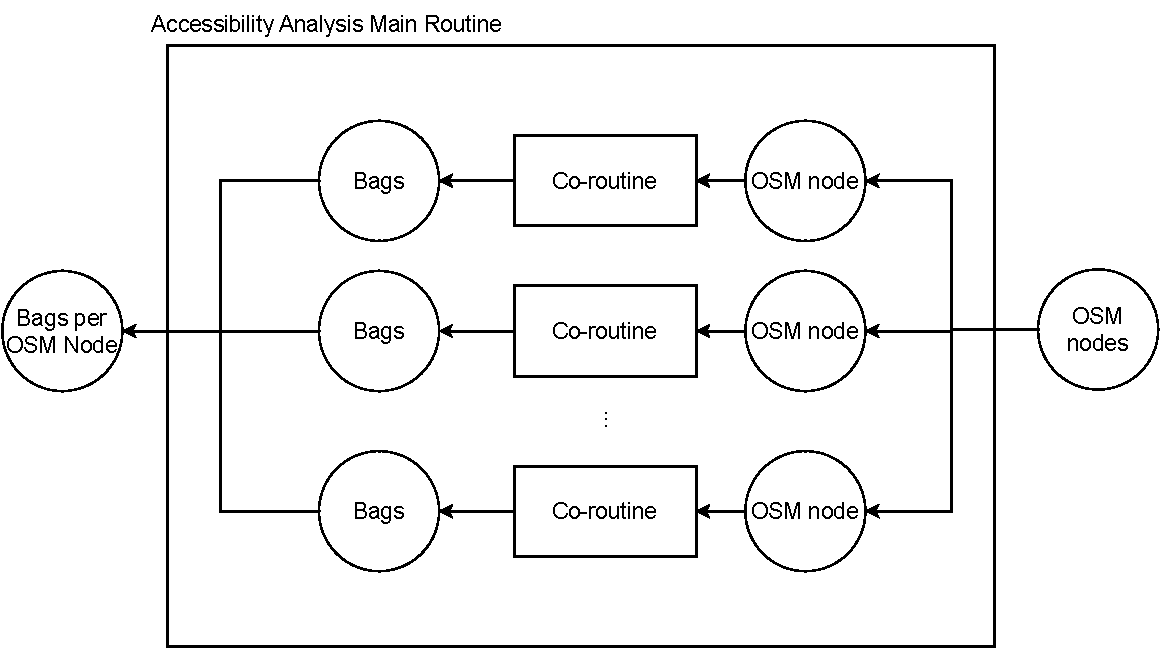
\includegraphics[scale=0.75]{Figures/method/main_routine}
    \caption{Main Routine}
    \label{fig:main_routine}
\end{figure}
The main routine, depicted in Figure \ref{fig:main_routine}, calls our scaffolding routing algorithm described in Section \ref{subsec:routing_algorithms} on each OSM node provided by the input routine.
This results in a set of Bags for each node.

% Metrics routine
\begin{figure}
    \centering
    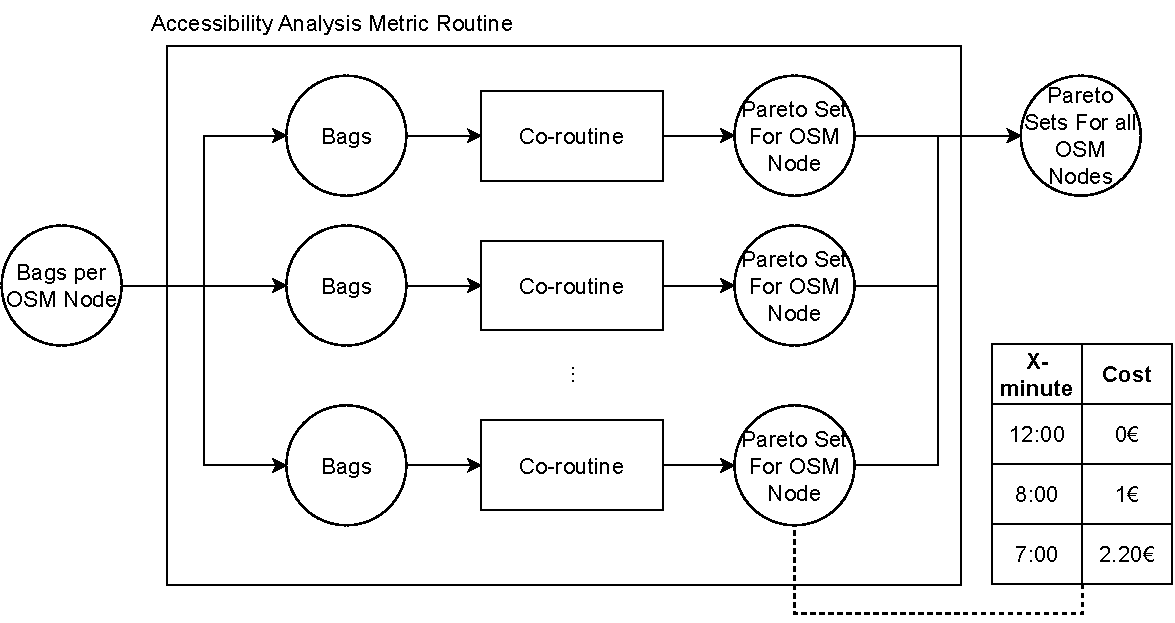
\includegraphics[scale=0.75]{Figures/method/metric_routine}
    \caption{Metric Routine}
    \label{fig:metric_routine}
\end{figure}
The metrics routine, depicted in Figure \ref{fig:metric_routine}, processes the bags into Pareto sets, where one entry in the Pareto set is a tuple of the X-minute city metric and the related cost.
To do so, we process each collection of bags separately - one co-routine for each OSM node/collection of bags.

\begin{figure}
    \centering
    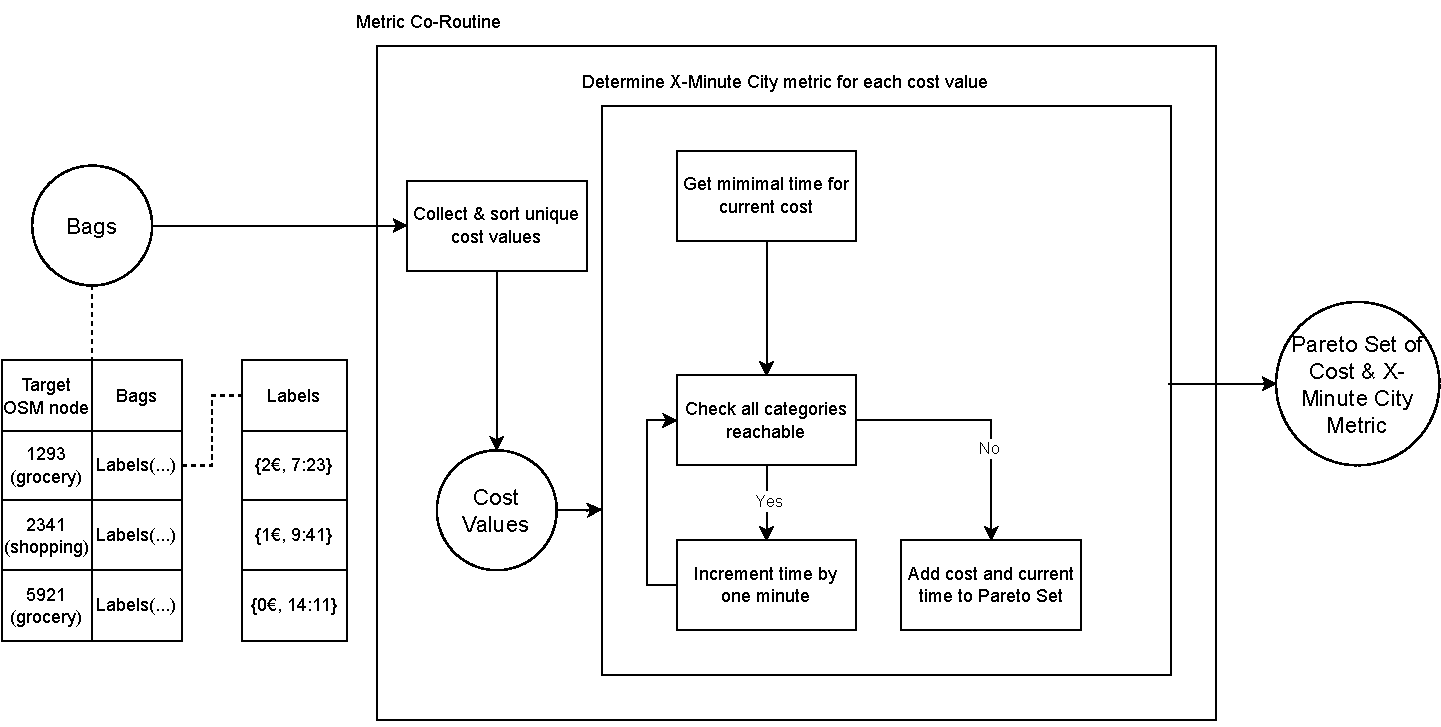
\includegraphics[scale=0.50]{Figures/method/metric_coroutine}
    \caption{Metric Co-Routine}
    \label{fig:metric_co_routine}
\end{figure}
The co-routine is depicted in Figure \ref{fig:metric_co_routine} and works as follows.
We start by collecting all unique cost values in each label in each bag and then sort them in ascending order.
For each cost value we then determine the associated X-minute city metric.
We do so by checking whether every category is reachable given the cost value and an iteratively increasing time value.
We start with a time value that is equal to the minimum time across all labels.
If all categories are reachable, we've found the X-minute city metric, which together with the cost value is added to the Pareto set.
If not, we increase the time value by one minute and check again.
We repeat this until all cost values are processed.
The result is a Pareto set for each OSM node/collection of bags.

\clearpage
\section{Experiment}
\label{sec:experiment}

We apply our method to the city of Cologne, to retrieve insights about how different modes of transport interact and how they contribute to the accessibility of the city.
As we want to compare different modes of transport, we will calculate the metric multiple times for different scenarios, each with a different combination of modes of transport.

\subsection{Scenarios}
\label{subs:scenarios}

No matter, the mode of transport, we always allow for walking, for two reasons.
First, walking is the most accessible mode of transport, available to almost everyone and without any additional costs.
Second, most other modes of transport require walking at some point, be it to the next bus stop or to the next available bicycle.

The first scenario we consider is our baseline scenario, which only considers walking.
This scenario measures what is possible without any additional infrastructure. 
Distinct from other scenarios, it does not require any additional cost, thus presenting the most basic form of urban mobility.

Building on this, the second scenario we consider is the scenario of only walking. 
We consider this scenario as the benchmark scenario, as we hope to achieve similar (or even better) results with more sustainable modes of transport.
Therefore, we use it to answer the question of how competitive sustainable modes of transport are in comparison to the traditional mode of travel by car. 

Transitioning from the simplest form of mobility, the third scenario, focused on public transport, becomes essential to understand the effectiveness and accessibility of urban transit systems. 
This scenario evaluates how well-connected and time-efficient public transportation networks are, and their role in reducing reliance on personal vehicles. 
It also investigates the impact of public transport on urban mobility and its potential in contributing to a more sustainable urban environment. 
Specifically, it assesses whether public transport is a viable alternative to the personal car and whether it actually offers significant advantages over walking, considering the X-minute city metric.

Next, in the fourth scenario, we shift our focus to the dynamics of bicycle sharing systems. 
This scenario is important for assessing the feasibility and attractiveness of cycling as a primary mode of transportation in urban areas. 
We will directly compare it to the public transport scenario, to understand which sustainable mode of transport is superior.

Finally, the fifth scenario combines public transport and bicycle sharing, offering insights into the synergy between these two modes of transport.
For the sake of brevity, we refer to this scenario as the combined scenario.
This integrated approach mirrors a growing trend in urban mobility solutions, where multi-modal transport options are increasingly favored. 
It underscores how this combination can bridge the gaps in accessibility and efficiency found when each mode is used independently. 
This scenario is expected to be the most competitive against cars, offering a comprehensive and sustainable urban transit model that could reshape the landscape of city mobility.

We summarize the scenarios in Table \ref{table:scenarios}.

\begin{table}[h]
\centering
\begin{tabular}{|p{4cm}|p{5cm}|p{4cm}|}
\hline
\textbf{Scenario} & \textbf{Modules} & \textbf{Key Points} \\
\hline
Walking & Walking & Baseline scenario \\
\hline
Personal Car & Personal Vehicle, Walking & Benchmark scenario \\
\hline
Public Transport & Public Transport, Walking & Evaluate the effectiveness public transport systems \\
\hline
Bicycle Sharing & Vehicle Sharing, Walking & Evaluate the effectiveness of bicycle sharing systems \\
\hline
Combined & Public Transport, Bicycle Sharing, Walking & Evaluate the effectiveness of sustainable multi-modal transport systems \\
\hline
\end{tabular}
\caption{Scenarios for Urban Mobility Analysis}
\label{table:scenarios}
\end{table}

The specific configuration of the module matrices for each scenario can be found in Appendix \ref{app:experiment_module_matrix_configuration}.

\subsection{Data}
\label{subs:data}

To calculate the Pareto sets of the X-minute city metric for the different scenarios, we use four different datasets.
First, we require data that depicts the street network of the city of Cologne.
Second, we need to know the locations of the POIs, which we want to reach.
Third, we need to know the locations of the public transport stops, as well as, the schedules of the public transport.
For the bicycle sharing scenario, we also need to know the locations of the bicycles.
Lastly, we also use land use data to identify where residential areas are located, so that we can calculate the X-minute city metric only for these areas.

As we will query spatial datasets of various formats, from different sources, the area covered by the datasets will not be the same.
Therefore, we first define an area of interest and later trim the datasets to this area.
In our case, this area is defined as the area of the administrative district of Cologne, specifically the "Stadtkreis Köln".
We retrieve the specific boundary of this area with the help of the Overpass API \shortcite{OverpassAPIOverpass}.
The specific query can be found in Appendix \ref{app:overpass_query} and the resulting region can be seen in Figure \ref{fig:area_plus_buffer}.

\begin{figure}
  \begin{center}
    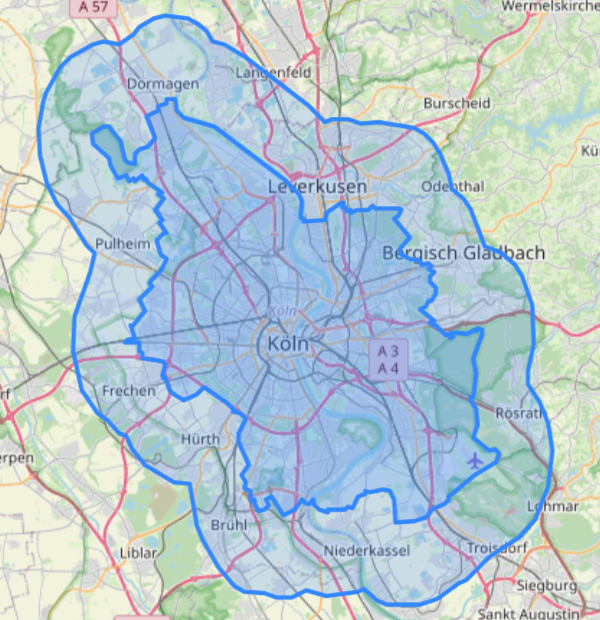
\includegraphics[width=0.55\textwidth]{Figures/experiment/area_plus_buffer.png}
  \end{center}
  \caption{Area of Interest and Buffer Region}\label{fig:area_plus_buffer}
\end{figure}

Additionally, the Figure also shows a buffer region around our area of interest.
This larger region adds a buffer of approximately 5 km and is used by some in parts of our data processing.


\subsubsection{Street Network \& POIs}
\label{subs:street_network_pois}

For the street network and the POIs, we use data from OpenStreetMap (OSM) \shortcite{OpenStreetMap}.
To use OSM data in practice various tools and services have been developed.
Among these we use, pyrosm \shortcite{Pyrosm} which is a Python library designed specifically for reading OSM data in different formats and conducting data processing operations.
Through pyrosm, we can automatically fetch data from sources like Geofabrik \shortcite{GeofabrikDownloadServer} and BBBike \cite{BBBikeExtractsOpenStreetMap}, which are two of the most popular OSM data providers.
In our case, we use the data for the city of Cologne from BBBike.
However, due to the flexibility of pyrosm, it is easily possible to use data from other sources as well and expand our analysis to other cities.

After retrieving the data, we retrieve a graph representation of the street network trimmed to the buffered area of interest.
Using the buffered region is important, because without it calculating the X-minute city metric at the border of the area of interest would result in a higher value than the actual value.
As a last cleaning step, we remove all nodes, that are not part of the largest weakly connected component.
A weakly connected component is a subgraph in which, if all directed edges were treated as undirected, any two vertices from the subgraph would be connected.
Multiple weakly connected components in graphs derived from OSM data, mostly happen at the border of the considered area and can be neglected.

Because we consider multiple different modes of transport on the network, it is important to filter out all edges that are not accessible by the respective mode of transport.
To do so, we use pyrosm's built-in filtering functionality.
For reproducibility, we list the filters that pyrosm uses in Appendix \ref{app:pyrosm_network_filter}.

To retrieve the POIs, we use the Overpass API \shortcite{OverpassAPIOverpass}.
We retrieve all POIs that fall into one of our predefined categories specified in Section \ref{subsec:metric} inside the area of interest plus the buffer mentioned before.

\subsubsection{Public Transport}
\label{subs:public_transport}

To handle public transport data, we use the General Transit Feed Specification (GTFS) \shortcite{GTFS}.
To retrieve it we rely on the Mobility Database \shortcite{MobilityDatabase}.
This database serves as an open-source repository containing links to publicly available GTFS feeds globally, standing as the subsequent version of TransitFeeds \shortcite{OpenMobilityDataPublicTransit}.
Similarly to the OSM data, we trim the GTFS data to the area of interest plus the buffer.
The GTFS data is also cleaned and converted into a format that is more suitable for our algorithm, or more specifically McRAPTOR, which is part of our algorithm.
Specifically, there are two major incompatibilities between the GTFS specification and RAPTOR's notion of routes and trips.
Firstly, each trip belonging to a single route in RAPTOR visits the same stops in the same order.
It is not possible that a trip skips some stops that another trip of the same route visits, much less use a completely different sequence of routes.
In GTFS routes do allow that, as they are much more a group of trips that is presented to the rider under the same name or identifier.
Secondly, GTFS trips allow visiting the same stop multiple times, which is not allowed in RAPTOR.
To overcome these difference we split up routes into smaller routes, that follow the same sequence of stops.
Additionally, e also remove circular trips, altogether.


\subsubsection{Bicycle Sharing}
\label{subs:bicycle_sharing}

Our bicycle sharing data was retrieved from the NextBike API over a time period of one year.
The data consists of all trips that were made with the NextBike system in the city of Cologne from the 15th of January 2022 to the 31st of August 2023.
To get representative samples of the locations of all bicycles we employ the following strategy.
We first discretize the data spatially and temporally.
For the temporal discretization, we derive the location of each bicycle every hour.
For the spatial discretization, we use H3 hexagons with a resolution of 9.
The resulting data is the information how many bicycles were at each hexagon at each hour.
This data is then used as an input for k-medoids clustering \shortcite{rdusseeun1987clustering} with a k of 4.
K-medoids, also known as PAM (Partitioning Around Medoids) algorithm, is a clustering technique that partitions a dataset into K clusters, where each is assigned a medoid, that is the most centrally located object in a cluster. 
Unlike K-means, which uses mean values as cluster centers, K-medoids an actual data point as the center of a cluster.
This has the advantage that the centers are part of the dataset and therefore are realistic samples.
We use the resulting medoids as different configurations of the locations of the bicycles.

\subsubsection{Land Use}
\label{subs:land_use}

To identify the residential areas, we use the land use data from the CORINE Land Cover (CLC) project \shortcite{CORINELandCover}.
The data covers the whole of Europe and is publicly available, which again makes it possible to expand our analysis to other cities in Europe.
We trimmed the data to the area of interest and then filtered for the land use types "Continuous Urban Fabric" and "Discontinuous Urban Fabric".
These two land use types represent the residential areas of the city.
The residential areas inside the area of interest are shown in Figure \ref{fig:input_hexagons_residential_areas}.
Additionally, the Figure shows the hexagons of resolution 9 that are found inside the residential areas.

\begin{figure}
  \begin{center}
    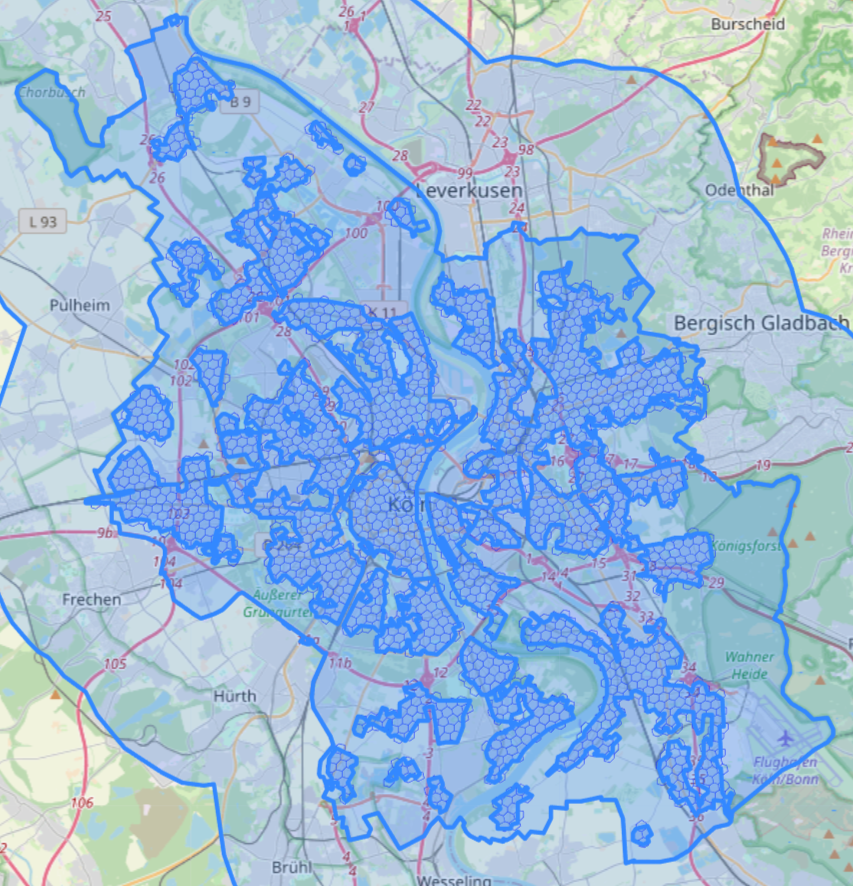
\includegraphics[width=0.65\textwidth]{Figures/experiment/input_hexagons_residential_areas.png}
  \end{center}
  \caption{Area of Interest and Buffer Region with Residential Areas and Input Hexagons}
  \label{fig:input_hexagons_residential_areas}
\end{figure}


\subsection{Assumptions}
\label{subs:assumptions}

To calculate the X-minute city metric we have to abstract from reality to some degree.
We do so by making the following plausible assumptions.

Firstly, we assume that travelling along an edge on the street network, by walking, cycling or driving, is always proportional to the length of the edge.
To obtain the time it takes to travel along an edge, we divide the length of the edge by the speed of the mode of transport.
The different speeds for the different modes of transport are listed in Table \ref{table:speeds}.

\begin{table}[h]
\centering
\begin{tabular}{|c|l|}
\hline
\textbf{Mode} & \textbf{Speed (m/s)} \\
\hline
Walking & 1.4 \\
\hline
Cycling & 4.0 \\
\hline
Driving & 11.0 \\
\hline
\end{tabular}
\caption{Speeds for Different Modes of Transport}
\label{table:speeds}
\end{table}

The walking speed is consistent with the measurement that \shortciteA{willberg15minuteCityAll2023} made in their study.

We also pose some assumption on the transitioning between different modes of transport, as well as, in the case of public transport, the transfer time at the stops.
For the transfer time at stops we assume a fixed time of one minute.
To transition from any OSM network-based mode of transport to public transport, we assume that the stop is precisely at the location the closest node of the OSM network.
As OSM networks contain public transport stops, there should be no difference between the two.
Similarly, we assume that the bicycles are located at the closest node of the OSM network.
As the OSM network, especially in city is very dense, this assumption is reasonable.
We also assume that bicycles and cars can be parked anywhere on their respective network for the sake of simplicity.


\subsubsection{Pricing}
\label{subs:pricing}

We try to implement a pricing scheme in our scenarios that represents the real-world circumstances as closely as possible.

For bicycle sharing, we use the pricing scheme of NextBike, which is 1euro every 15 minutes.
To depict this we add a hidden value to the labels processed in MLC that depicts how long the current bicycle trip is.
As two consecutive bicycle trips are considered separately we nullify this hidden value after each run of MLC.

For public transport, we use the pricing scheme of the Cologne Transport Authority (KVB), which is 2.20euro for trips that span four stops or less.
For any trip that spans more than four stops or any multitude of trips the KVB charges 3.20euro.
To depict this we add a hidden values to the labels processed in McRAPTOR that depicts how many stops the traveler already traversed.
Because two consecutive trips are considered together, we don't need to nullify the hidden value.

% TODO: personal car

\clearpage
\section{Results}
\label{sec:results}

This section presents the findings received when carrying out our experiment, addressing the research questions outlined in the introduction.
Recall, our primary inquiries revolved around understanding the role of bicycle sharing and public transport in shaping cities into 15-minute cities (RQ\ref{rq:bicycle_pt}), the impact of cost on accessibility (RQ\ref{rq:cost_accessibility}), the measurement of accessibility considering multiple transport modes and associated costs (RQ\ref{rq:measure_accessibility}), and deriving specific urban planning recommendations for Cologne (RQ\ref{rq:recommendations}).

The results are the output of our experiment, which consists of a novel method for accessibility-based planning that incorporates multiple modes of transport while also considering cost.
The data retrieved from our experiments consists of two parts.
Firstly, for each sub-scenario and hexagon, we get the Pareto set of the X-minute city metric and cost.
Secondly, we also retrieve a Pareto set for each (sub)-scenario, hexagon, and additionally category.
%We use this second version for an extensive cost analysis in Section \ref{sec:monthly_costs}.
In the following subsections, we first observe our method's runtime and memory usage and then analyze the output of our method.

\subsection{Runtime Observations}
\label{subsec:runtime_observations}

% TODO: data prep is missing
% TODO fill in actual numbers
Observing the runtime and memory usage required to run our experiment enables us to evaluate the practicality of our approach.
To execute our experiment, we used a machine with an AMD Ryzen 7 5800H CPU and 32 GB of RAM.
As explained in Section \ref{sec:method}, our routine is split into three parts: the input, main, and metric routine.
The input routine is the only routine that we are able to reuse across different sub-scenarios, which means that we only had to run it once.
It took under two minutes to run and required no more than 19 gigabytes of memory.
The main routine took the longest, with 6 hours and 11 minutes, and required around 70 gigabytes of memory at max.
More than half of the memory used by the main routine was provided as swap memory.
Also, we only utilized 8 of the 16 available cores for parallelization.
Lastly, the metric routine took under 15 minutes to run and required no more than 20 gigabytes of memory.
We found that the high memory consumption of the main routine primarily stems from the graph-based representation of the street network of Cologne.

\subsection{X-Minute City Metric}
\label{subsec:15_minute_city_metric}

% table (mean, quantiles) of the optimal X-minute city metric
We first analyze the optimal X-Minute city metric, which is the lowest value for the X-minute city metric in each Pareto set.
This means that we disregard the incurred costs.
Table \ref{tab:optimal_x_minute_city_metric} shows the mean, as well as the 25\%, 50\%, and 75\% quantiles of the optimal X-minute city, each scenario over all hexagons.
Our findings indicate that cars enable the fastest access to all necessary Points of Interest (POIs), with an average optimal X-minute city time of 3 minutes and 12 seconds. 
This mode of transport significantly outpaces other methods, establishing a benchmark for urban mobility efficiency.
However, it should be taken into consideration that our car scenario is very optimistic, and these numbers should be viewed with caution

\begin{table}
  \caption{Optimal X-minute City Metric Over All Hexagons Disregarding Cost}
  \label{tab:optimal_x_minute_city_metric}
  \begin{center}
    \begin{tabular}{lrrrr}
    & mean & 25\% & 50\% & 75\% \\
    scenario &  &  &  &  \\
    Bicycle & 12m 26s & 7m 15s & 10m 45s & 15m 30s \\
    Car & 3m 11s & 2m 00s & 3m 00s & 4m 00s \\
    Combined & 11m 30s & 7m 15s & 10m 17s & 14m 20s \\
    Public Transport & 12m 47s & 9m 00s & 12m 00s & 16m 00s \\
    Walking & 14m 05s & 9m 00s & 12m 00s & 17m 00s \\
    \end{tabular}
  \end{center}
\end{table}

In contrast, sustainable modes of transport, such as bicycles, public transport, a combination of bicycles and public transport, and walking, demonstrate similar accessibility times. 
These modes record average times ranging from 11 minutes and 30 seconds to 14 minutes, with walking being the least time-efficient mode with an average of 14 minutes and 5 seconds. 
Integrating bicycles with public transport emerges as the most time-efficient sustainable mode, with an average time of 11 minutes 30 seconds. 

A direct comparison between public transport and walking shows that the time savings offered by public transport are 1 minute and 18 seconds. 
However, this benefit is not evenly distributed across all areas.
The analysis of quantiles reveals that the time improvement only establishes at the 75\% quantile with a 1-minute gain, while the 25\% and 50\% quantiles do not show any improvements.

Similarly, adding public transport to bicycle sharing, i.e., comparing the combined scenario with the bicycle sharing scenario, improves the average optimal time to reach all categories by 56 seconds.
Again, this improvement is not evenly distributed but only applies to the 50\% worst hexagons.
Specifically, we see no improvement from bicycle sharing to public transport in the 25\% quantiles, and the improvement in the 50\% quantile is very minor with 28 seconds.
The improvement in the 75\% quantile is the largest with 1 minute and 10 seconds.
While there is an improvement in the mean and 75\% quantile, it is not as large as the improvement from walking to public transport.

We can make the same observation from the standpoint of adding bicycle sharing to walking and public transport.
Adding bicycle sharing to public transport, i.e., comparing the combined scenario with the public transport scenario, the data indicates an improvement in the average accessibility time, reducing it by 1 minute and 16 seconds.
In contrast to the previously discussed example of adding public transport to bicycles, this improvement already occurs for the 25\% quantile and is, therefore, more evenly distributed across all hexagons.

Adding bicycles to the walking scenario, i.e., comparing the bicycle scenario to the walking scenario, presents an average time reduction of 1 minute and 38 seconds, which denotes a significant enhancement in the accessibility metric. 
Again, this improvement already occurs at the 25\% quantile, showing that the improvements gained through bicycle sharing are more evenly distributed across all hexagons.

% -----
% visualization of the distribution of the optimal X-minute city metric
We can observe a similar pattern when visualizing the distribution of the optimal X-minute city metric in Figure \ref{fig:optimal_x_minute_city_metric}.
\begin{figure}
  \begin{center}
    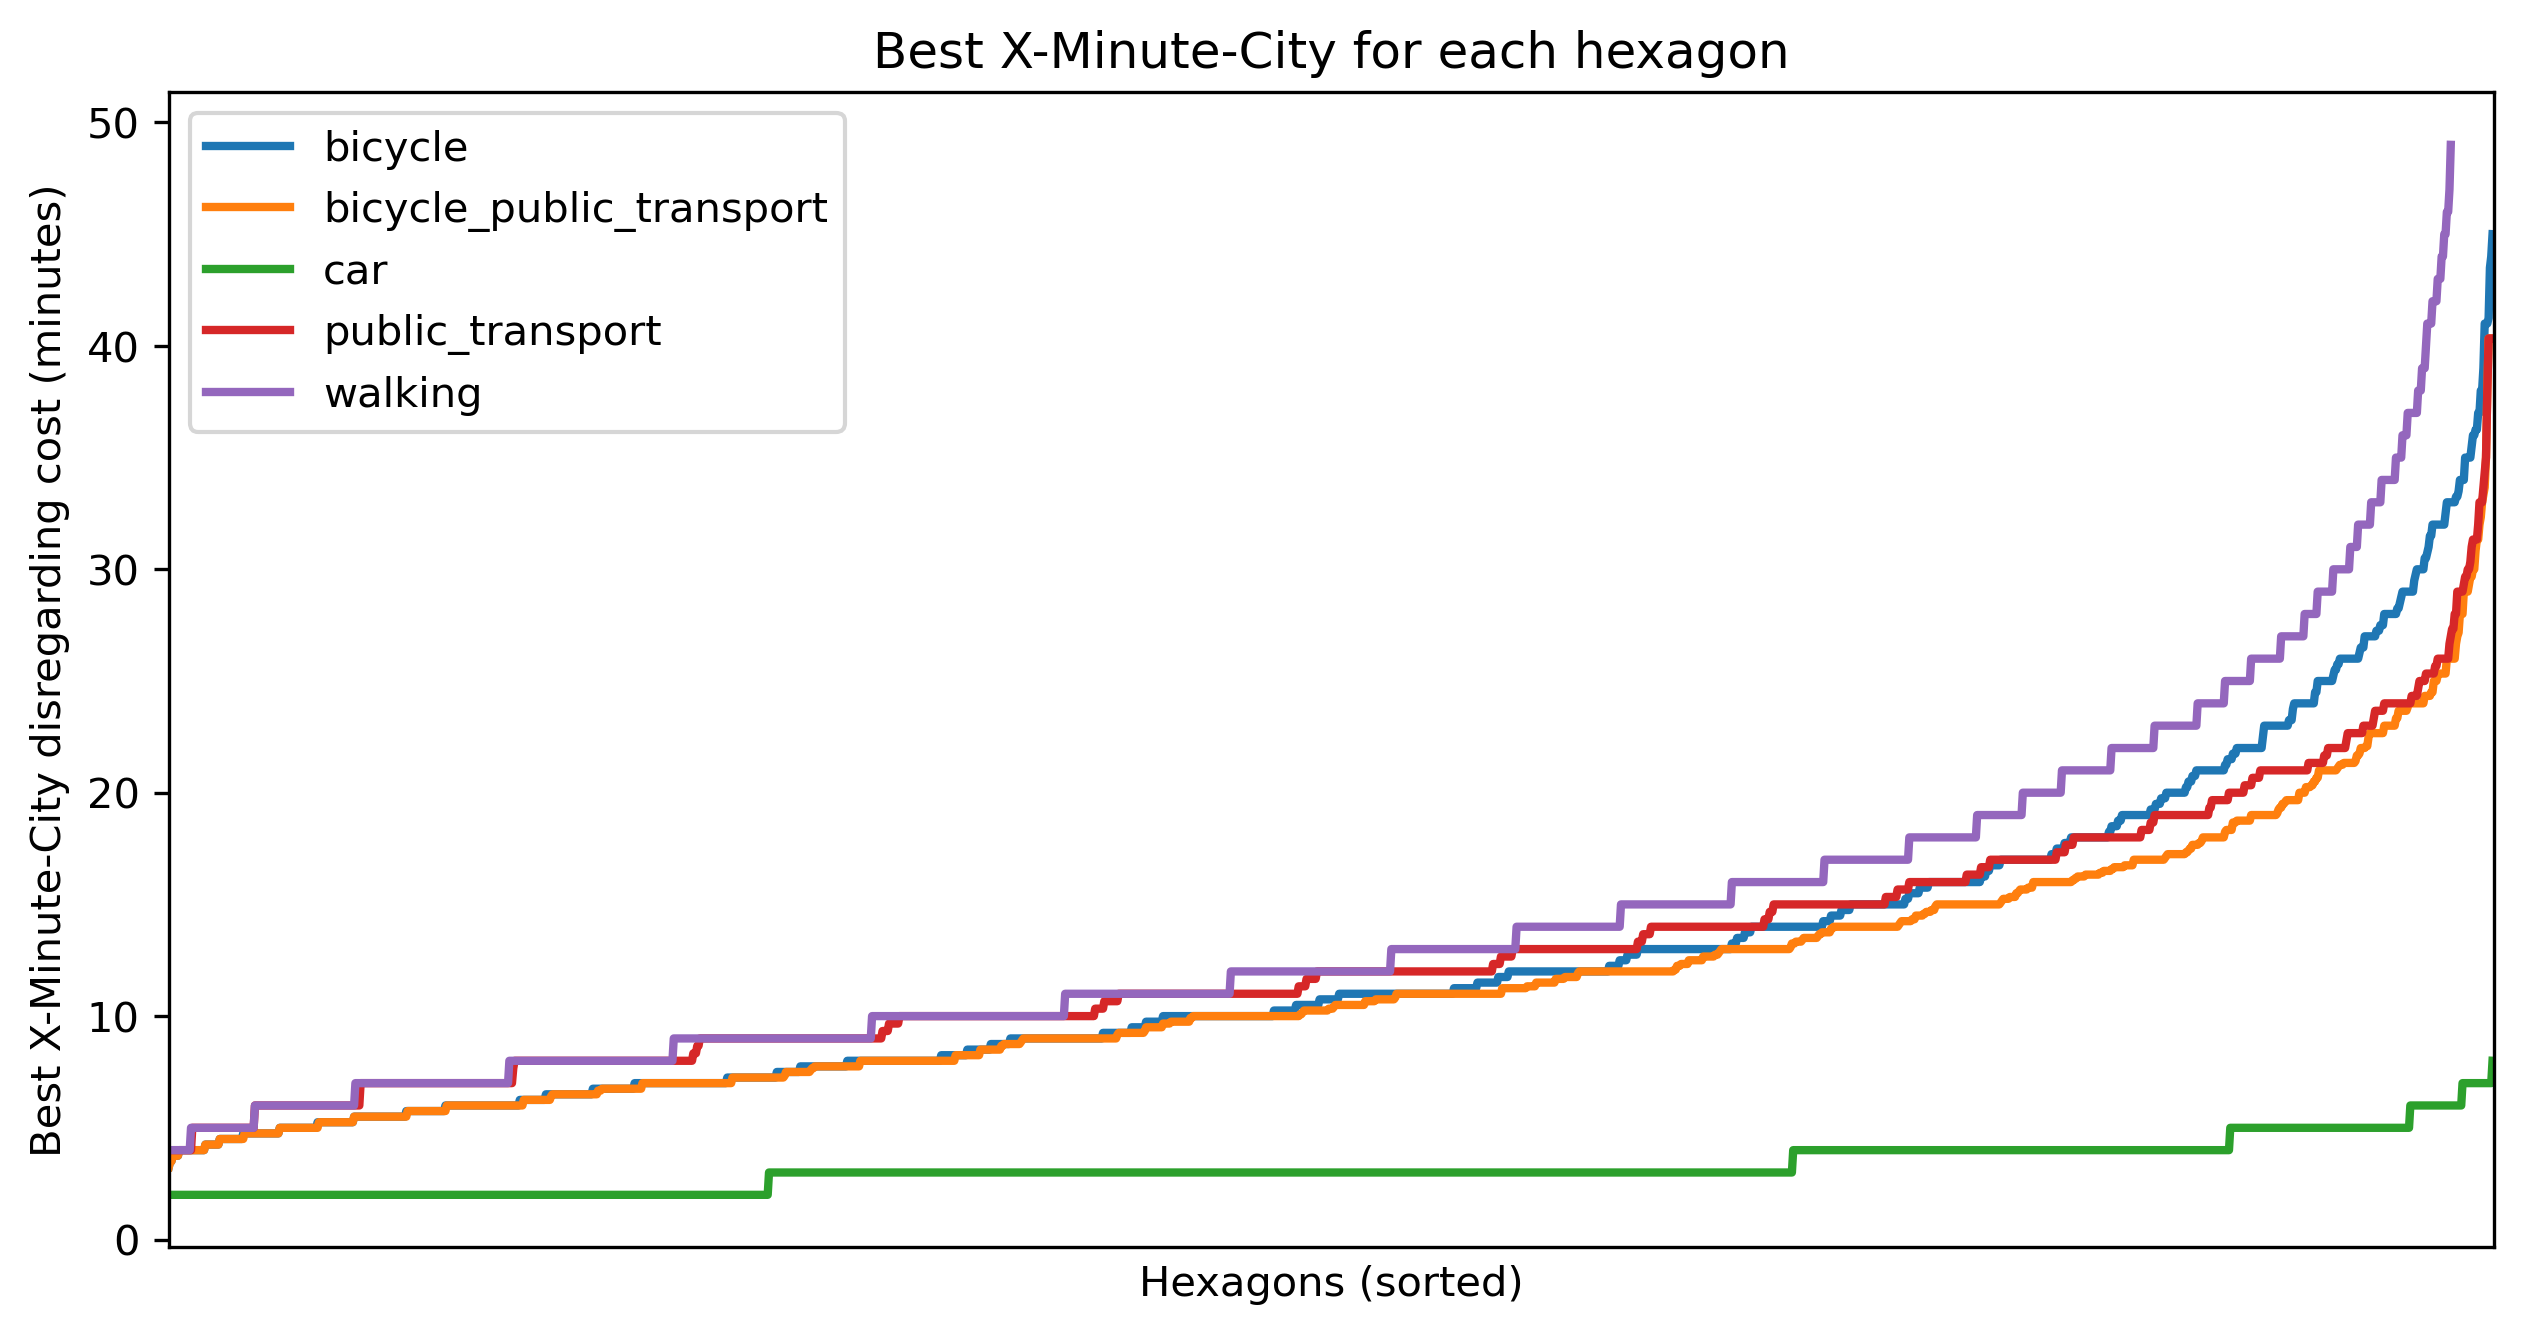
\includegraphics[width=0.85\textwidth]{Figures/results/minute_city_metric/best_x_minute_city}
  \end{center}
  \caption{Distribution of Optimal X-Minute City Metric}
  \label{fig:optimal_x_minute_city_metric}
\end{figure}
From the graph, it is evident that public transport and walking are the same for the more accessible hexagons to the left.
However, public transport results in lower X-Minute city metric values compared to walking for the less accessible hexagons to the right.
Hence, public transport outperforms walking in this situation.
In addition, the public transport scenario is worse than the pure bicycle sharing scenario but catches up and even overtakes it as we move to less accessible hexagons.
The same pattern can be observed when comparing the bicycle-sharing scenario to the combined scenario of bicycle-sharing and public transport.
For the most accessible hexagons to the left, the combined scenario is the same as the bicycle-sharing scenario, but as we move to less accessible hexagons to the right, the combined scenario results in lower values for the X-Minute city metric.
Similarly, when comparing the bicycle-sharing scenario to the combined scenario, we see that the combined scenario provides much better accessibility initially, but as we move to the least accessible hexagons, both become the same.
Generally, adding public transport can slow down the drastic increase of the optimal X-minute city metric at the end of the distribution.


Figure \ref{fig:optimal_map} shows the optimal X-minute city metric for each hexagon for the combined mode, which represents the best among all sustainable travel options.
\begin{figure}
  \begin{center}
    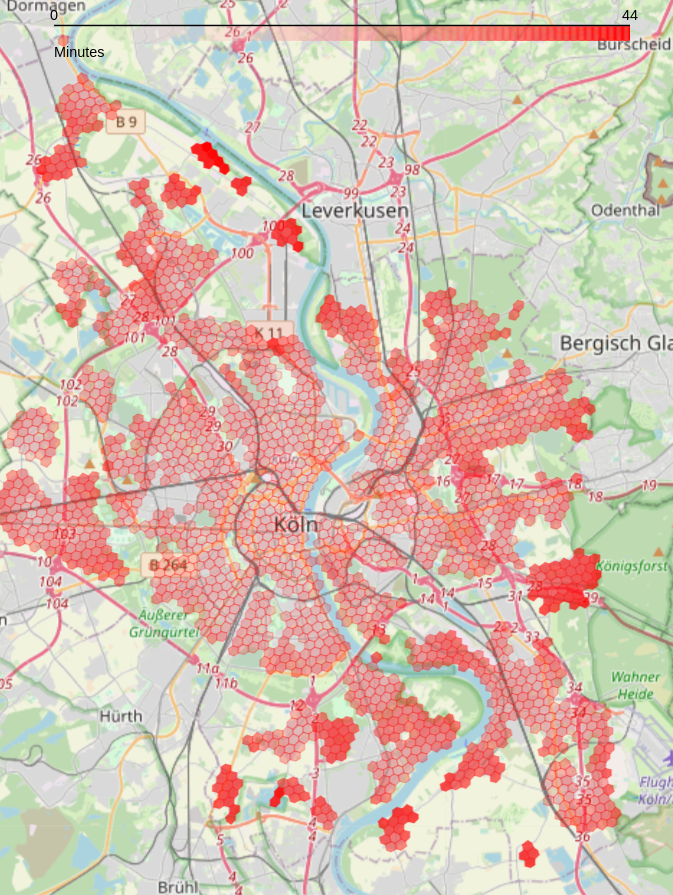
\includegraphics[width=0.45\textwidth]{Figures/results/minute_city_metric/optimal_map}
  \end{center}
  \caption{Map of Optimal X-Minute City Metric}
  \label{fig:optimal_map}
\end{figure}
We can see that the least accessible hexagons require 44 minutes to reach all categories if only sustainable modes of travel are used.
The least accessible regions are suburban areas in the north, south, and west of Cologne. 
The region on the left bank of the Rhine River next to Leverkusen, which is the district of Merkenenich, is especially inaccessible.

Figure \ref{fig:optimal_map_per_scenario} shows multiple maps of the optimal X-minute city metric for each hexagon, one for bicycle sharing, one for public transport, and one for walking.
\begin{figure}
     \centering
     \begin{subfigure}[b]{0.3\textwidth}
         \centering
         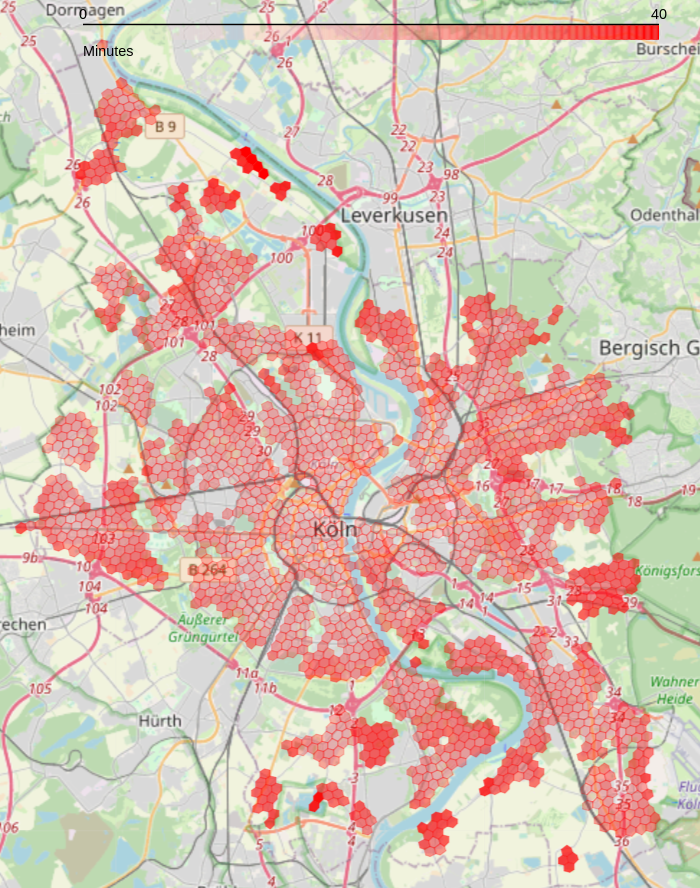
\includegraphics[width=\textwidth]{Figures/results/minute_city_metric/public_transport_optimal_map}
         \caption{Public Transport}
         \label{fig:public_transport_optimal_map}
     \end{subfigure}
     \hfill
     \begin{subfigure}[b]{0.3\textwidth}
         \centering
         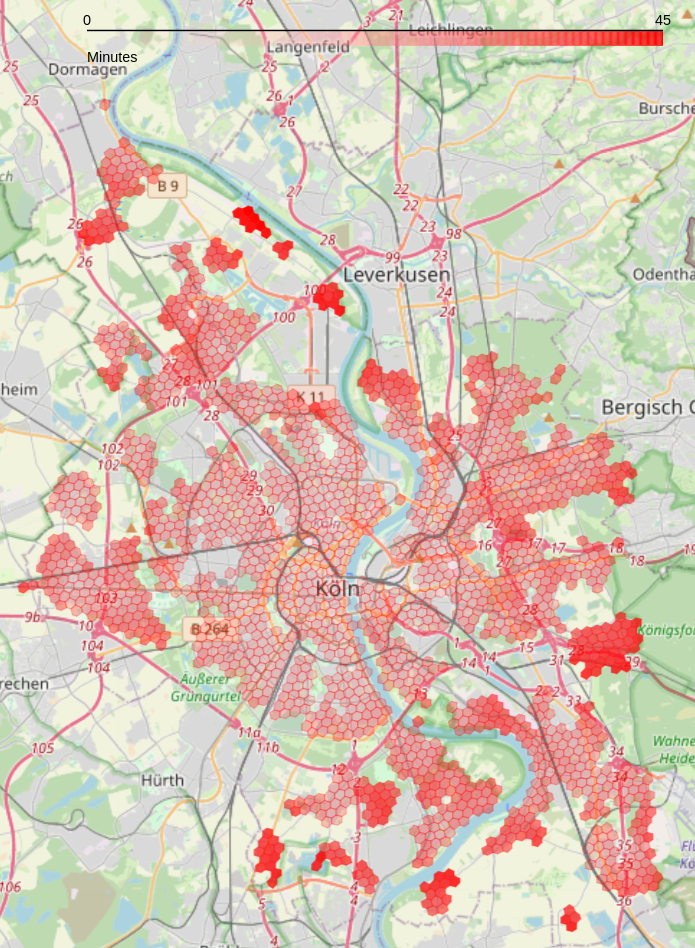
\includegraphics[width=\textwidth]{Figures/results/minute_city_metric/bicycle_optimal_map}
         \caption{Bicycle Sharing}
         \label{fig:bicycle_optimal_map}
     \end{subfigure}
     \hfill
     \begin{subfigure}[b]{0.3\textwidth}
         \centering
         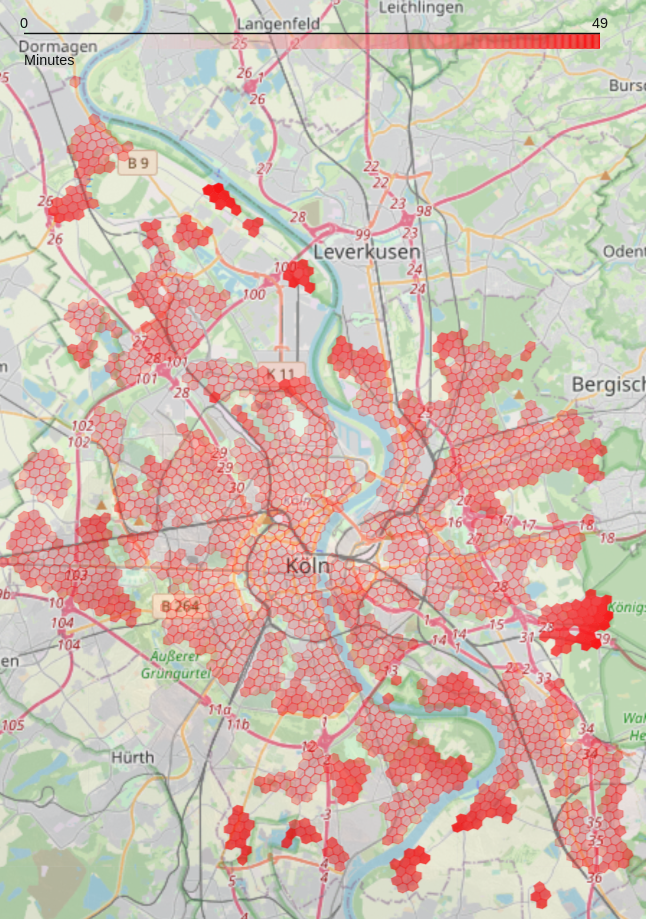
\includegraphics[width=\textwidth]{Figures/results/minute_city_metric/walking_optimal_map}
         \caption{Walking}
         \label{fig:walking_optimal_map}
     \end{subfigure}
        \caption{Map of Optimal X-Minute City Metric per Scenario}
        \label{fig:optimal_map_per_scenario}
\end{figure}
The areas in and around the city center are more accessible by bicycle sharing than by public transport and walking.
In the east of the city, near the forest "Königsforst", we see the district of Rath/Neumar, with low accessibility for all scenarios.
However, one can see that the region is more accessible by public transport than by bicycle sharing and walking.

\subsection{Cost}
\label{subsec:cost_of_15_minute_city}

% table (mean, quantiles) of required cost
Table \ref{tab:required_cost} shows the mean, the 25\%, 50\%, and 75\% quantiles and the maximum of the costs that are required to achieve the optimal value for the X-minute city shown in Section \ref{subsec:15_minute_city_metric}.
\begin{table}
  \caption{Required Cost for Optimal Over All Hexagons}
  \label{tab:required_cost}
  \begin{center}
    \begin{tabular}{lrrrrr}
     & mean & 25\% & 50\% & 75\% & max \\
    scenario &  &  &  &  &  \\
    Bicycle & 0.39 & 0.00 & 0.50 & 0.75 & 1.00 \\
    Car & 0.36 & 0.19 & 0.38 & 0.38 & 1.14 \\
    Combined & 0.86 & 0.00 & 0.75 & 1.30 & 3.95 \\
    Public Transport & 0.64 & 0.00 & 0.00 & 1.47 & 3.20 \\
    Walking & 0.00 & 0.00 & 0.00 & 0.00 & 0.00 \\
    \end{tabular}
  \end{center}
\end{table}
We can immediately see that there is no cost for hexagons at the 25\% and 50\% quantile when using public transport, implying that public transport is not used at all for those hexagons.
Looking at the 75\% quantile and the maximum required cost for an optimal X-Minute City metric for public transport, we see that the earlier observed benefits come at a cost.
Similarly, bicycle sharing and the combined mode have zero cost at the 25\% quantile, implying that they are not used for those hexagons.

Looking at the maximum cost values of each sustainable mode of transport shows us that bicycles never require more than \euro{1}.
As \euro{1} allows to travel a maximum of 15 minutes, it is never necessary to travel longer than 15 minutes after a bicycle is reached.
The maximum cost incurred by public transport is \euro{3.20}, which shows that the long-distance ticket of public transport (more than four stops) is used.
Similarly, in the combined scenario, the long-distance ticket is used with a 15-minute ride of bicycle sharing in at least one sub-scenario, resulting in the maximum price of \euro{3.95}.
Remember that the values we observe are average values of all sub-scenarios belonging to a scenario.
Because of this, the maximum price is \euro{3.95} and not \euro{4.20} (\euro{1} + \euro{3.20}), as not all sub-scenarios reach the maximum of \euro{4.20}.

We can make similar observations with more granularity when looking at the distribution of the required cost in Figure \ref{fig:maximum_required_cost_for_x_minute_city}.
\begin{figure}
  \begin{center}
    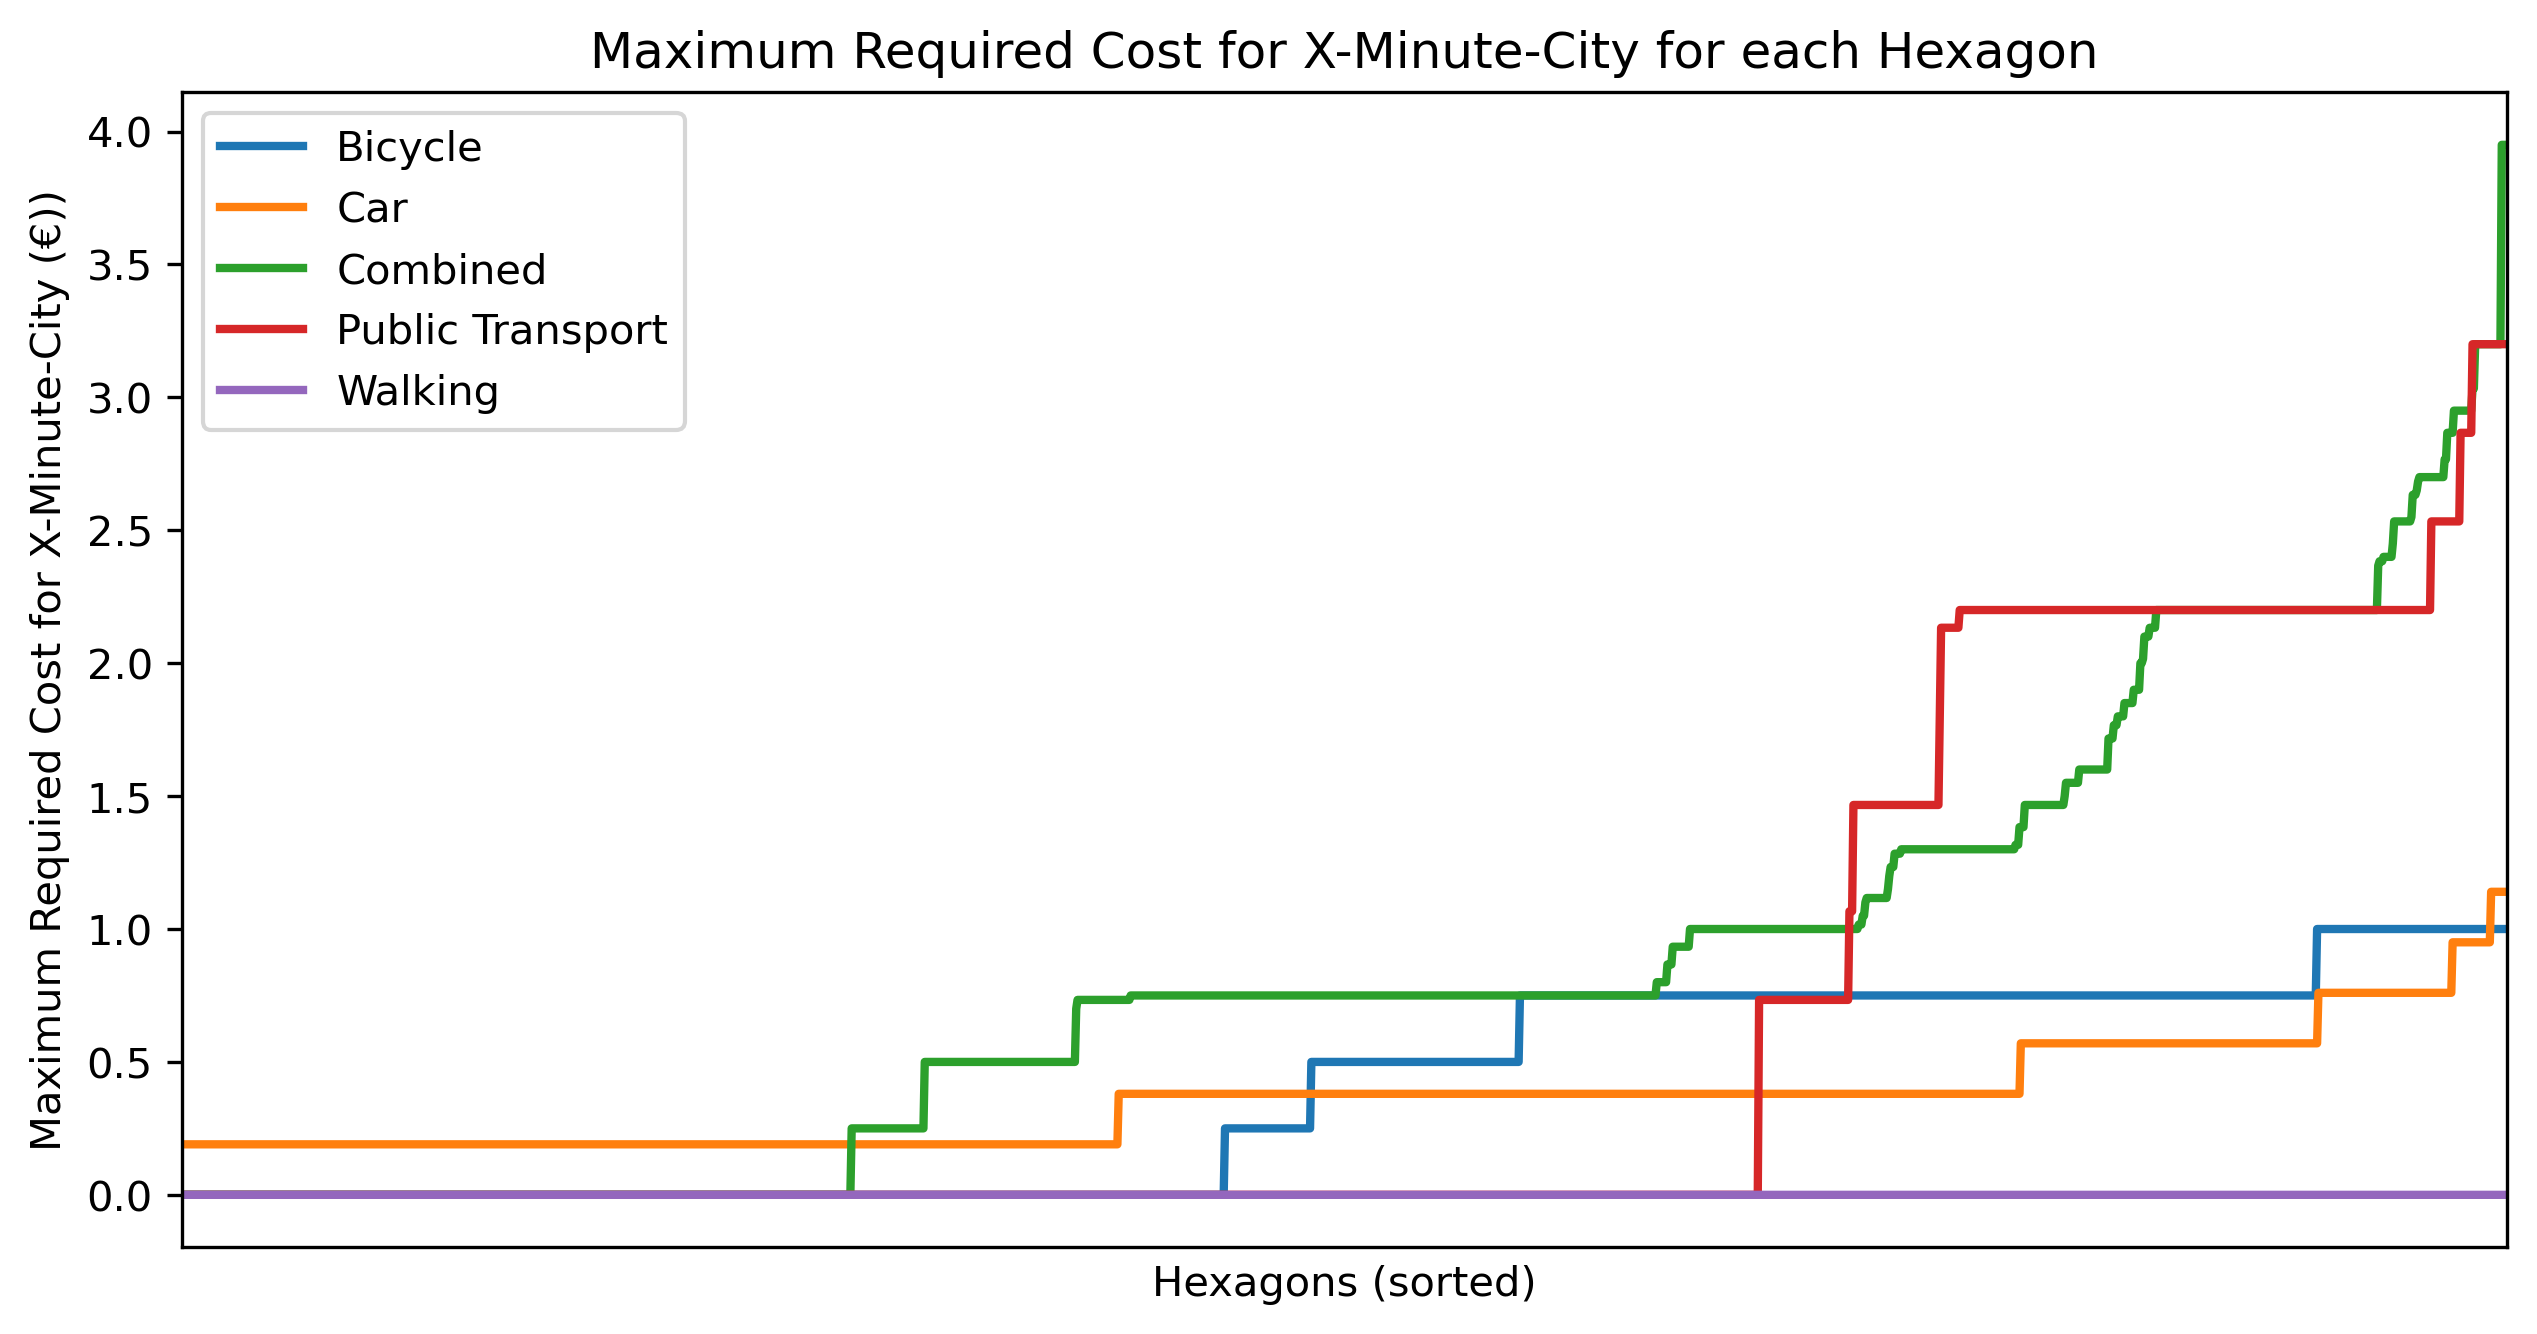
\includegraphics[width=0.65\textwidth]{Figures/results/cost/maximum_required_cost_for_x_minute_city}
  \end{center}
  \caption{Maximum Required Cost for Optimal X-Minute City Metric}
  \label{fig:maximum_required_cost_for_x_minute_city}
\end{figure}
A new pattern stands out when comparing public transport and the combined mode.
We see that the combined mode has higher costs earlier, surpassed by public transport, only to be surpassed again by the combined mode.
% discussion stuff (not sure where to put this)
%The first price increase in the combined mode can be explained by the \euro{1} cost of 15-minute bicycle sharing.
%Then public transport's costs surpassed those of the combined mode the combined mode. 
%This is probably because bicycle sharing is more cost-efficient and can somewhat replace public transport.
%The fact that the combined mode then surpasses public transport again most likely stems from the fact that the combined mode can achieve faster access than public transport by using bicycle sharing, which is more expensive than a short-distance ticket alone.
% END

Figure \ref{fig:cost_map_per_scenario} shows the cost required to reach the optimal X-minute city metric for each hexagon for public transport, bicycle sharing, and the combined scenario of bicycle sharing and public transport.
Note that we do not show the cost for the walking scenario, as it is always \euro{0}.
In these figures, we see that sometimes the cost is zero.
As the portrayed scenarios all have costs associated with them, a cost of zero means that only walking is used.
\begin{figure}
     \centering
     \begin{subfigure}[b]{0.3\textwidth}
         \centering
         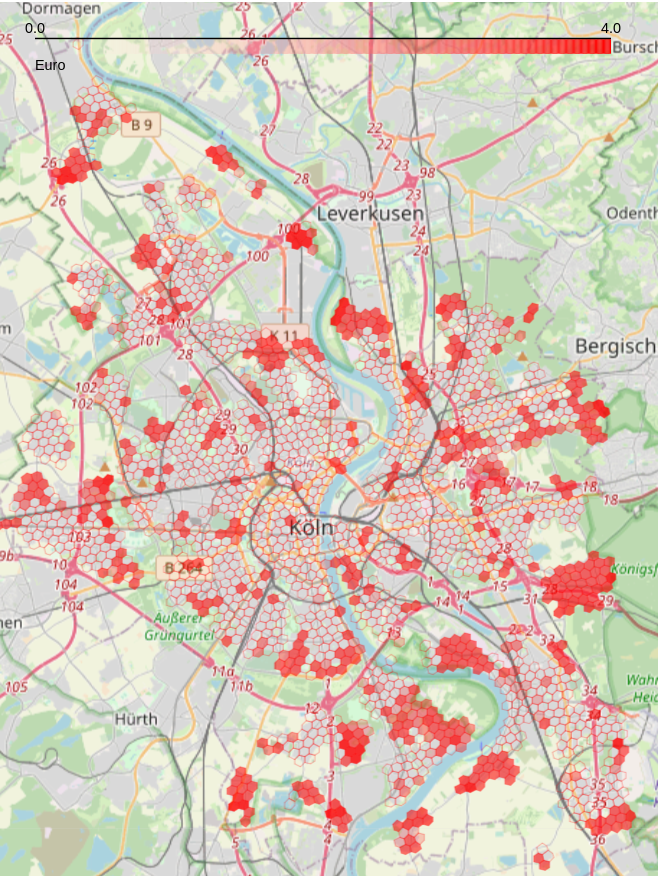
\includegraphics[width=\textwidth]{Figures/results/cost/public_transport_cost_map}
         \caption{Public Transport}
         \label{fig:public_transport_cost_map}
     \end{subfigure}
     \hfill
     \begin{subfigure}[b]{0.3\textwidth}
         \centering
         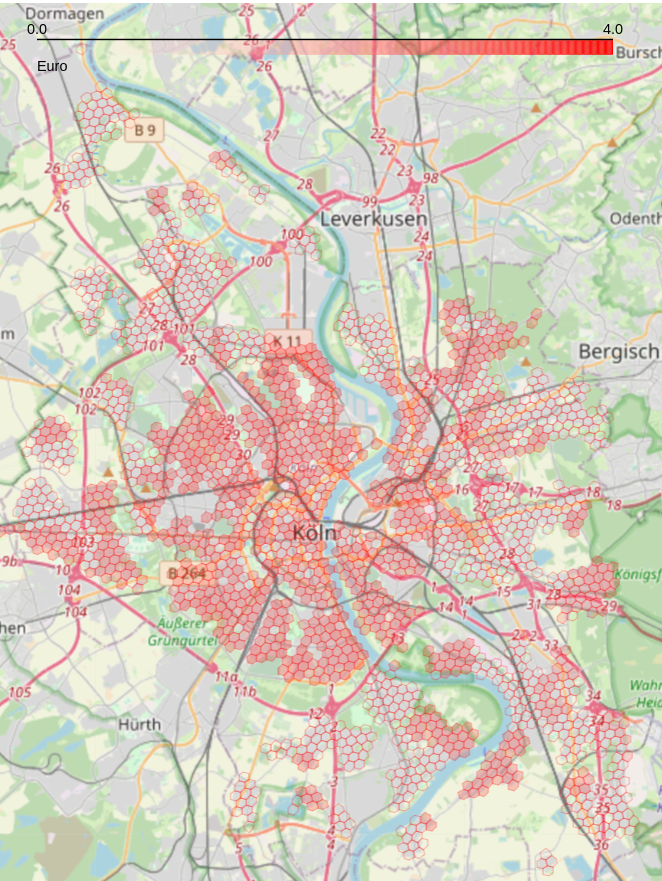
\includegraphics[width=\textwidth]{Figures/results/cost/bicycle_cost_map}
         \caption{Bicycle Sharing}
         \label{fig:bicycle_cost_map}
     \end{subfigure}
     \hfill
     \begin{subfigure}[b]{0.3\textwidth}
         \centering
         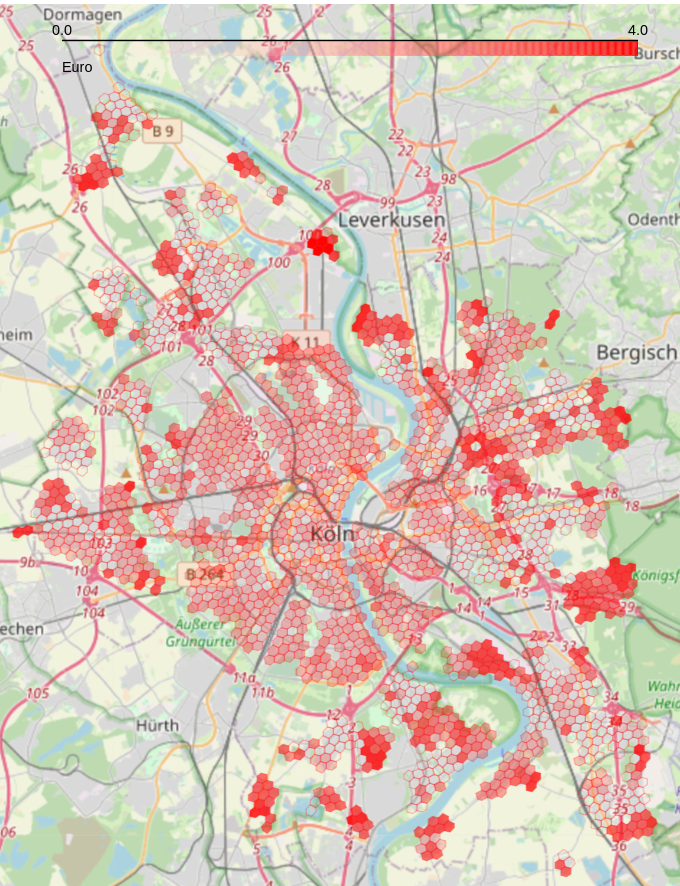
\includegraphics[width=\textwidth]{Figures/results/cost/bicycle_public_transport_cost_map}
         \caption{Combined}
         \label{fig:bicycle_public_transport_cost_map}
     \end{subfigure}
       \caption{Map of Required Cost for Optimal for Each Hexagon}
        \label{fig:cost_map_per_scenario}
\end{figure}
We see almost in all hexagons in and around the city center, where NextBike's flex zone is located, the cost for the bicycle sharing scenario is \euro{1}.
This sometimes also extends outside the city center.
The cost of public transport is more scattered around the whole region. 
We can mostly see single hexagons in the city center and small groups of hexagons outside the city that have costs higher than zero.
For the combined mode, we see a pattern that is roughly equal to the union of the public transport and bicycle-sharing scenario.

\subsection{Interaction Between Cost and X-Minute City Metric}
\label{subsec:interaction_between_cost_and_15_minute_city_metric}

Next, we examine the interaction between the cost and the optimal X-minute city metric.
To do so, we investigate the mean Pareto front of the X-minute city metric and cost over all hexagons.
Before performing the analysis for the whole region of Cologne, we first examine the Pareto front of a single hexagon, which is depicted in Figure \ref{fig:example_pareto_front}.
The x-axis shows the cost, and the y-axis shows the X-minute city metric.
The line shows us what X-minute city metric is achievable for a given cost in a specific scenario.

\begin{figure}
  \begin{center}
     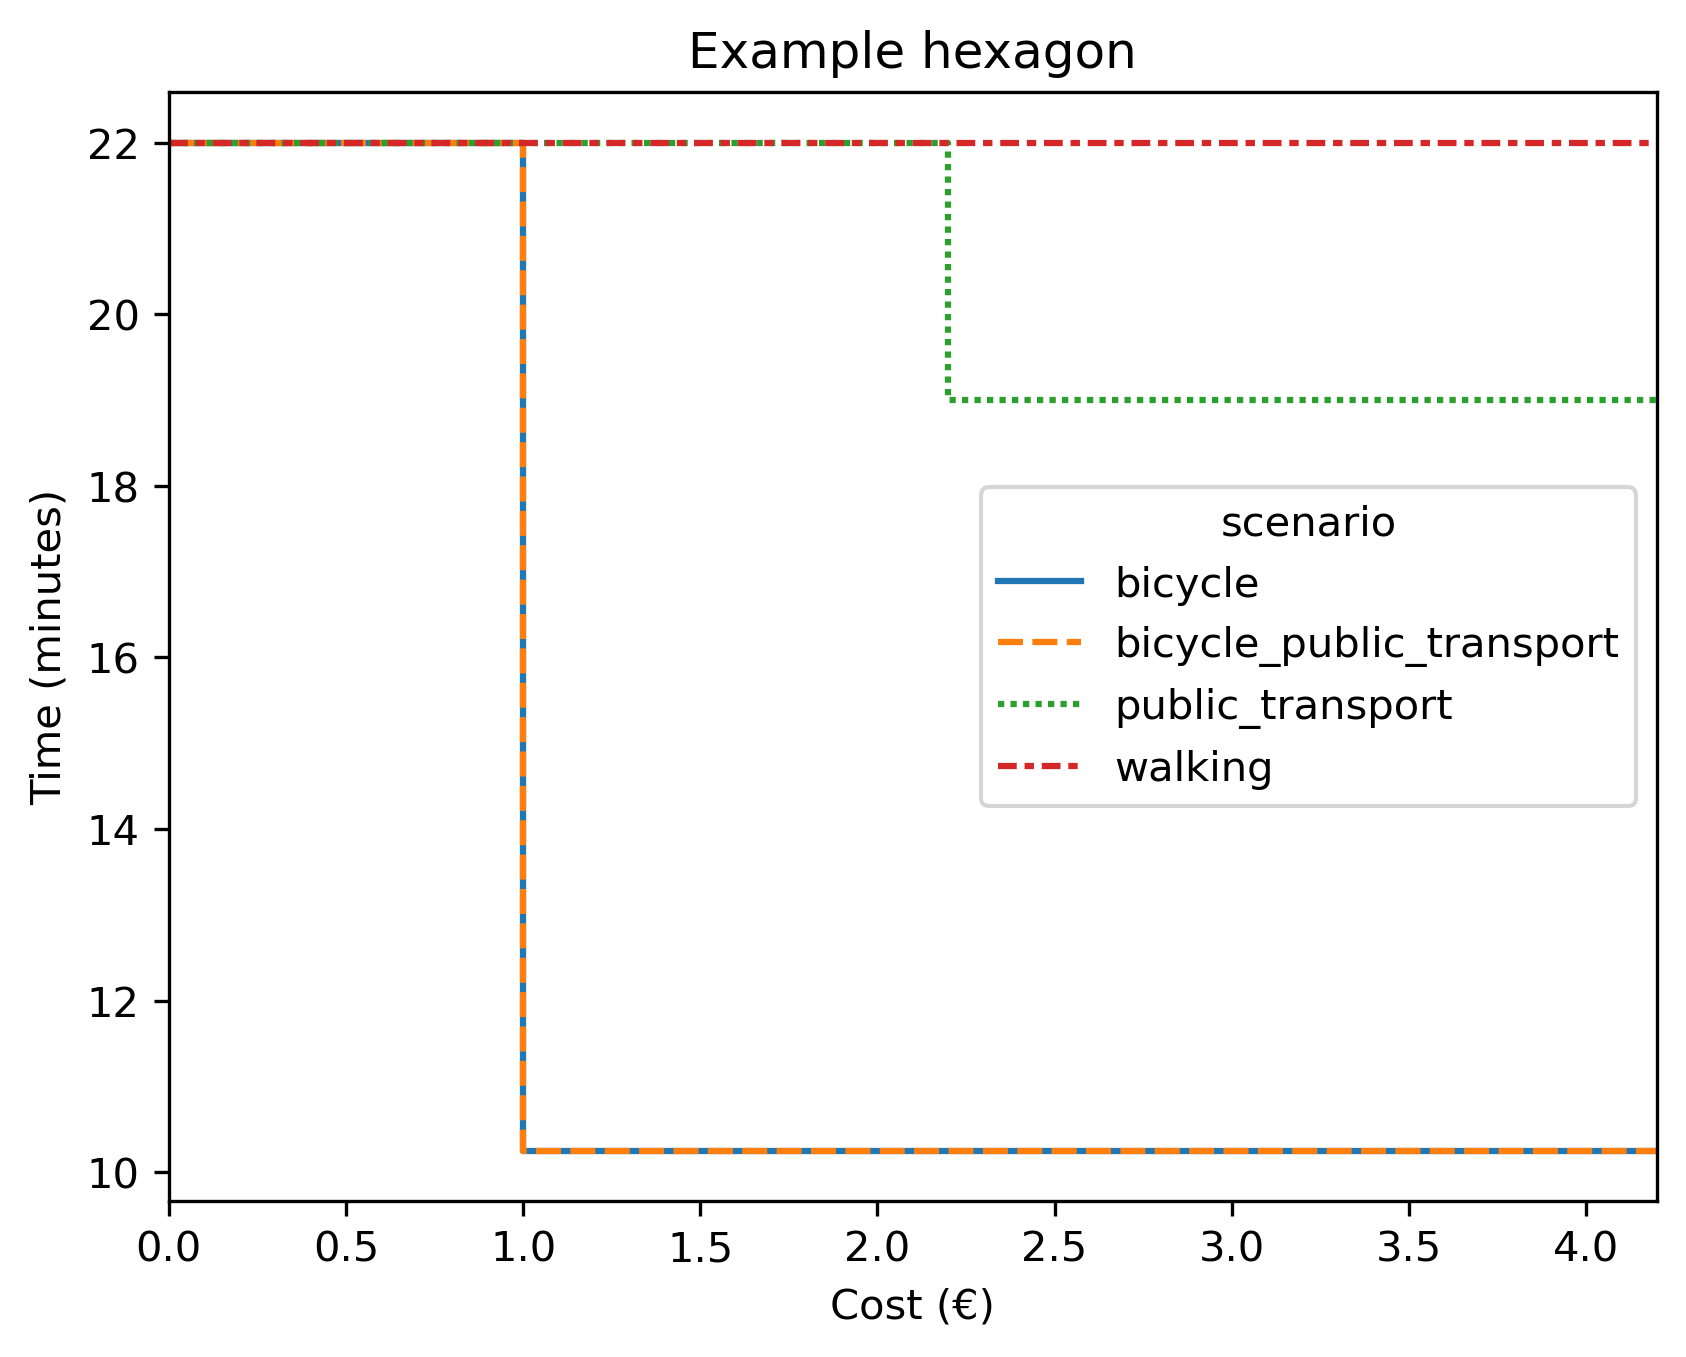
\includegraphics[width=0.5\textwidth]{Figures/results/metric_cost/example_profile}
  \end{center}
  \caption{Example Pareto Front}
  \label{fig:example_pareto_front}
\end{figure}

In our example, all modes begin with an accessibility value of 22 minutes for a cost of \euro{0}.
Increasing the cost only yields improvements when reaching a cost of \euro{1}, where the bicycle and combined scenarios can reach all categories within approximately 10 minutes.
Further, increasing the price to \euro{2.20} improves the public transport scenario, where reaching all categories within approximately 19 minutes is now possible.
Further cost increases do not yield any improvements for any scenario.

We can also quantify the value of the improvements as seen in Table \ref{tab:differences_in_example_hexagon}.
This table shows all the steps visible in the previous graph with their cost and magnitude of improvement.
In addition, we can calculate the benefit in minutes per one euro of cost to make the value of the steps more comparable.
\begin{table}
  \caption{Steps in Example Hexagon}
  \label{tab:differences_in_example_hexagon}
  \begin{center}
    \begin{tabular}{lrrrl}
     Scenario & Improvement & At cost (\euro) & Improvement (min/\euro) \\
     Bicycle & 11m 45s & 1.00 & 11.75 \\
     Combined & 11m 45s & 1.00 & 11.75 \\
     Public Transport & 3m 00s & 2.20 & 1.36 \\
    \end{tabular}
  \end{center}
\end{table}
As we can see, the bicycle and combined scenarios increase at a cost of \euro{1} is larger than the public transport scenario's increase and has a higher value per euro.

% generalization
To generalize these findings over all hexagons, we take the average over the X-minute city for each cost and scenario to generate an average Pareto front.
The resulting Pareto front can be seen in Figure \ref{fig:mean_time_per_cost}.
\begin{figure}
  \begin{center}
     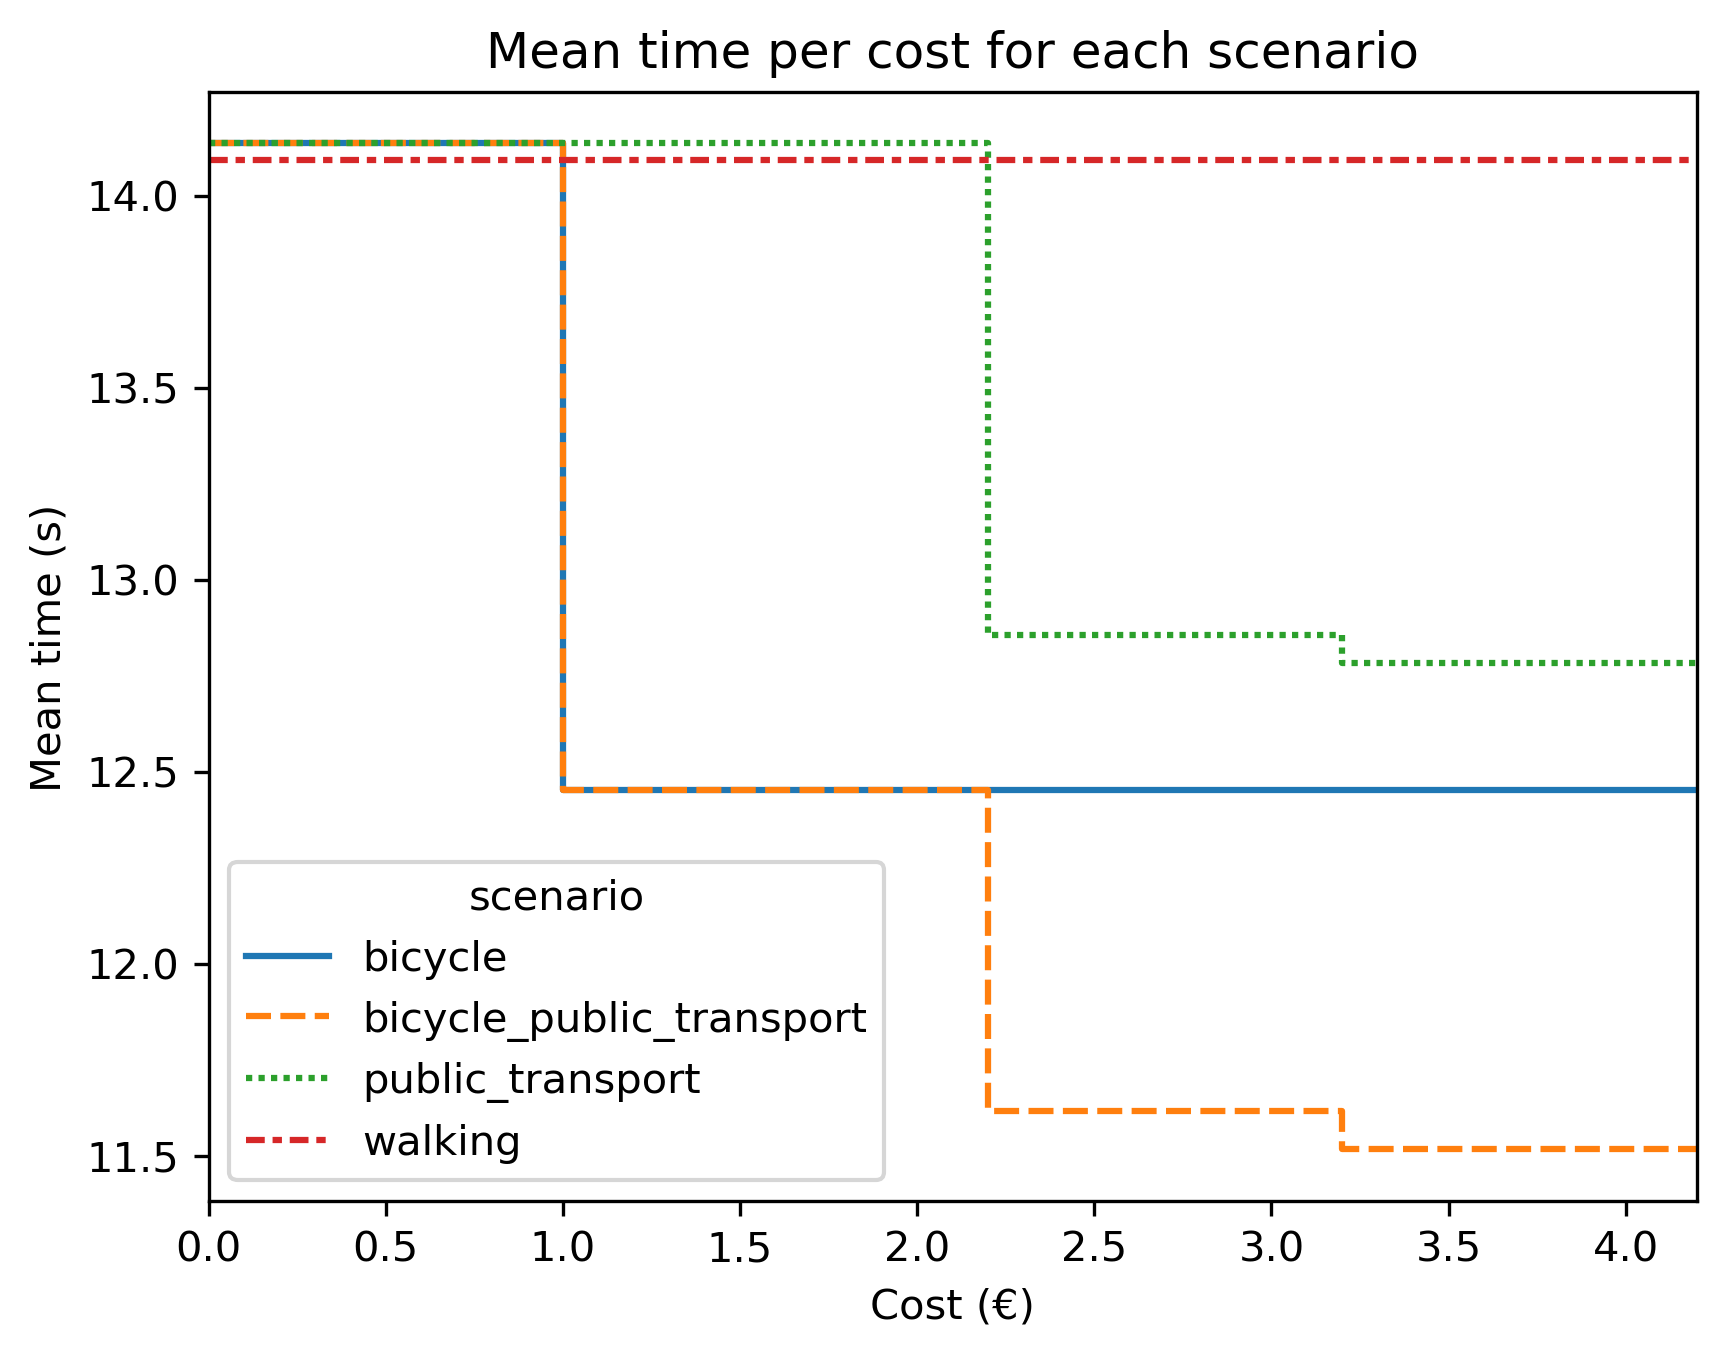
\includegraphics[width=0.5\textwidth]{Figures/results/metric_cost/mean_time_per_cost}
  \end{center}
  \caption{Mean Time per Cost for All Scenarios}
  \label{fig:mean_time_per_cost}
\end{figure}
Similarly to the example of the single hexagon from before, we can see improvements for the bicycle scenario and the combined scenario at the cost of \euro{1} of about 1 minute and 30 seconds.
We can also see the improvements in public transport at a cost of \euro{2.20}.
Unlike in the example of the single hexagon, we can also see the improvement at the cost of \euro{2.20} for the combined scenario.
Lastly, there is a slight improvement for the public transport scenario and the combined scenario at a cost of \euro{3.20}.

To compare these improvements, we can again look at the differences in Table \ref{tab:differences_in_mean_pareto_front}.
We do not analyze the differences in the combined scenario, as prior improvements of other modes skew the improvements, which results in numbers that are hard to interpret.

\begin{table}
  \caption{Steps in Mean Pareto Front}
  \label{tab:differences_in_mean_pareto_front}
  \begin{center}
    \begin{tabular}{|l|r|r|r|r|l|}
     \hline
     Scenario & Improv. & At cost (\euro) & Cost diff. (\euro) & Improv. (min/\euro) \\
     \hline
     Bicycle & 1m 41s & 1.00 & 1.00 & 1m 41s \\
     \hline
     Public transport & 1m 16s & 2.20 & 2.20 & 0m 34s \\
     \hline
     Public transport & 0m 04s & 3.20 & 1.00 & 0m 04s \\
     \hline
    \end{tabular}
  \end{center}
\end{table}

We see that the improvements of the bicycle scenario at the cost of \euro{1} are the largest, with an improvement of 1 minute and 41 seconds, and also the most cost-effective, with a value of 1 minute and 41 seconds per euro.
They are followed by the improvements of the public transport scenario at a cost of \euro{2.20} with an improvement of 1 minute and 16 seconds and a value of 34 seconds per euro.
The improvement at a cost of \euro{3.20} is minimal and the least cost-effective.

Next, we are going to look at the quantiles of the aggregated Pareto front.
Figure \ref{fig:quantile_time_per_cost} shows the 25\%, 75\%, and 90\% quantiles of the aggregated Pareto front.
The 25\% quantile gives us insights about the more accessible areas in the city.
Note that because we aggregate all the values of the X-minute city metric for a single cost and scenario at a time, the 25\% quantile Pareto front does not necessarily reflect the same 25\% of hexagons for each cost.

\begin{figure}
     \centering
     \begin{subfigure}[b]{0.48\textwidth}
         \centering
         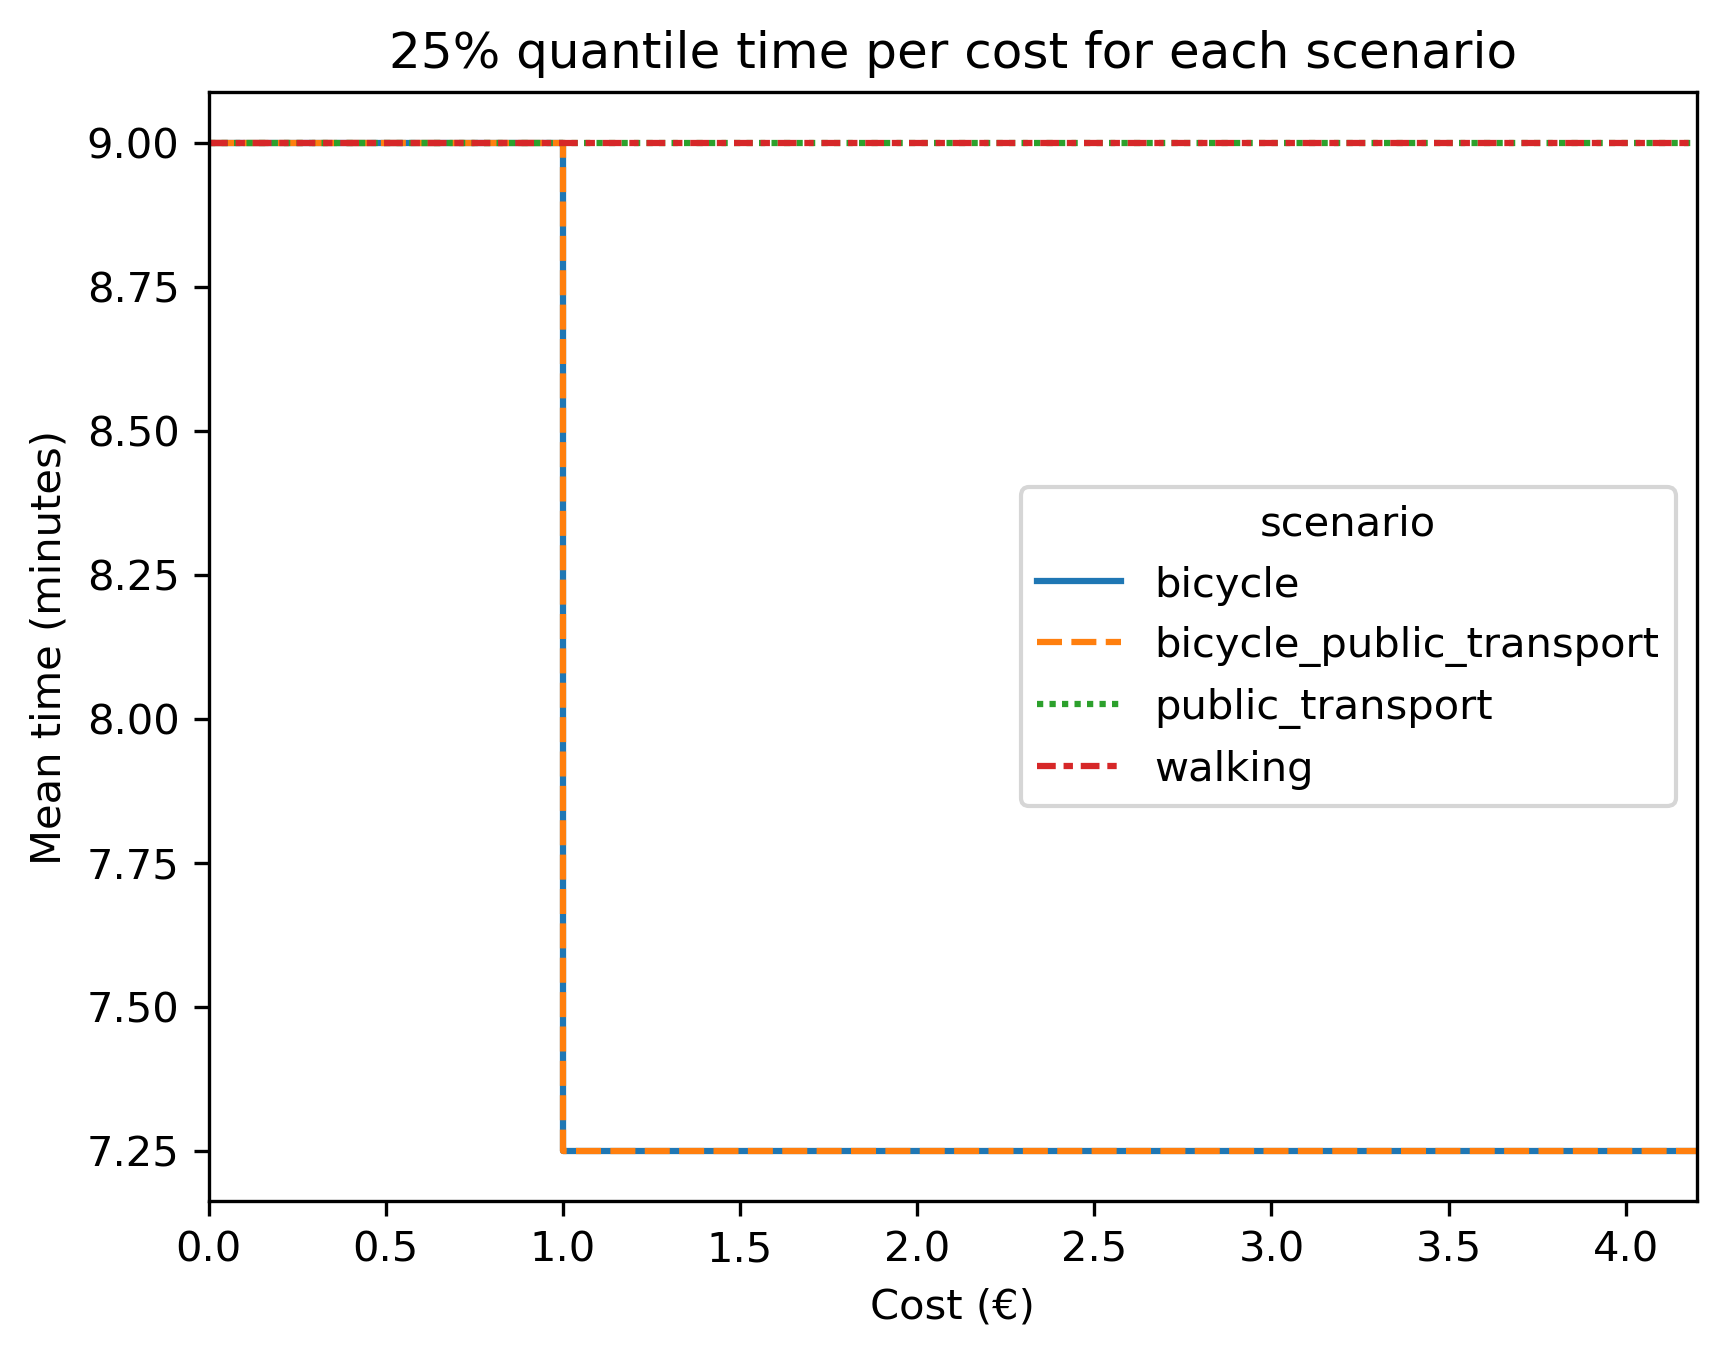
\includegraphics[width=\textwidth]{Figures/results/metric_cost/quantile_25_time_per_cost_for_each_scenario_without_car.png}
         \caption{25\% quantile time per cost for all scenarios}
         \label{fig:25_quantile_time_per_cost}
     \end{subfigure}
     \hfill
     \begin{subfigure}[b]{0.48\textwidth}
         \centering
         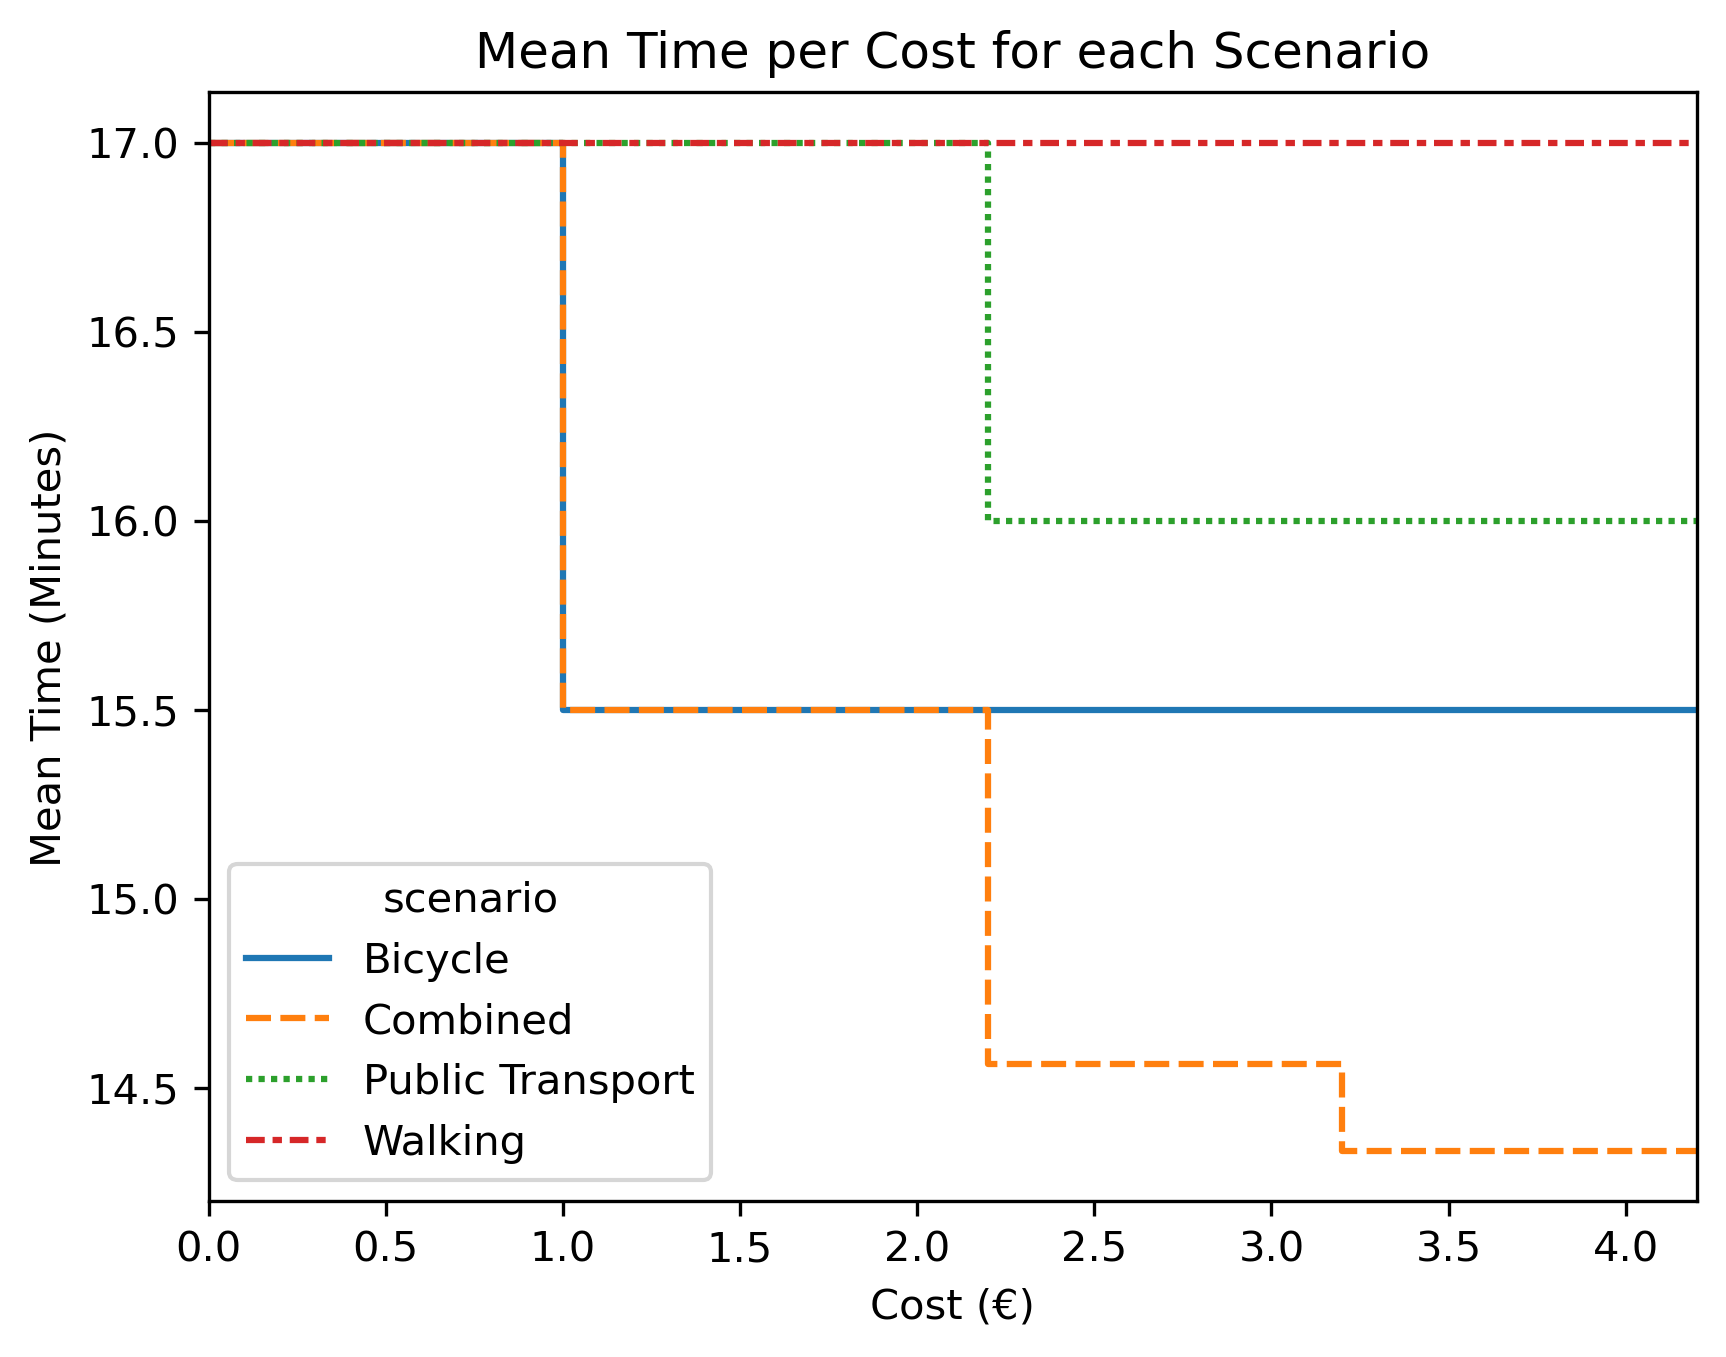
\includegraphics[width=\textwidth]{Figures/results/metric_cost/quantile_75_time_per_cost_for_each_scenario_without_car.png}
         \caption{75\% quantile time per cost for all scenarios}
         \label{fig:75_quantile_time_per_cost}
     \end{subfigure}
     \hfill
     \begin{subfigure}[b]{0.48\textwidth}
         \centering
         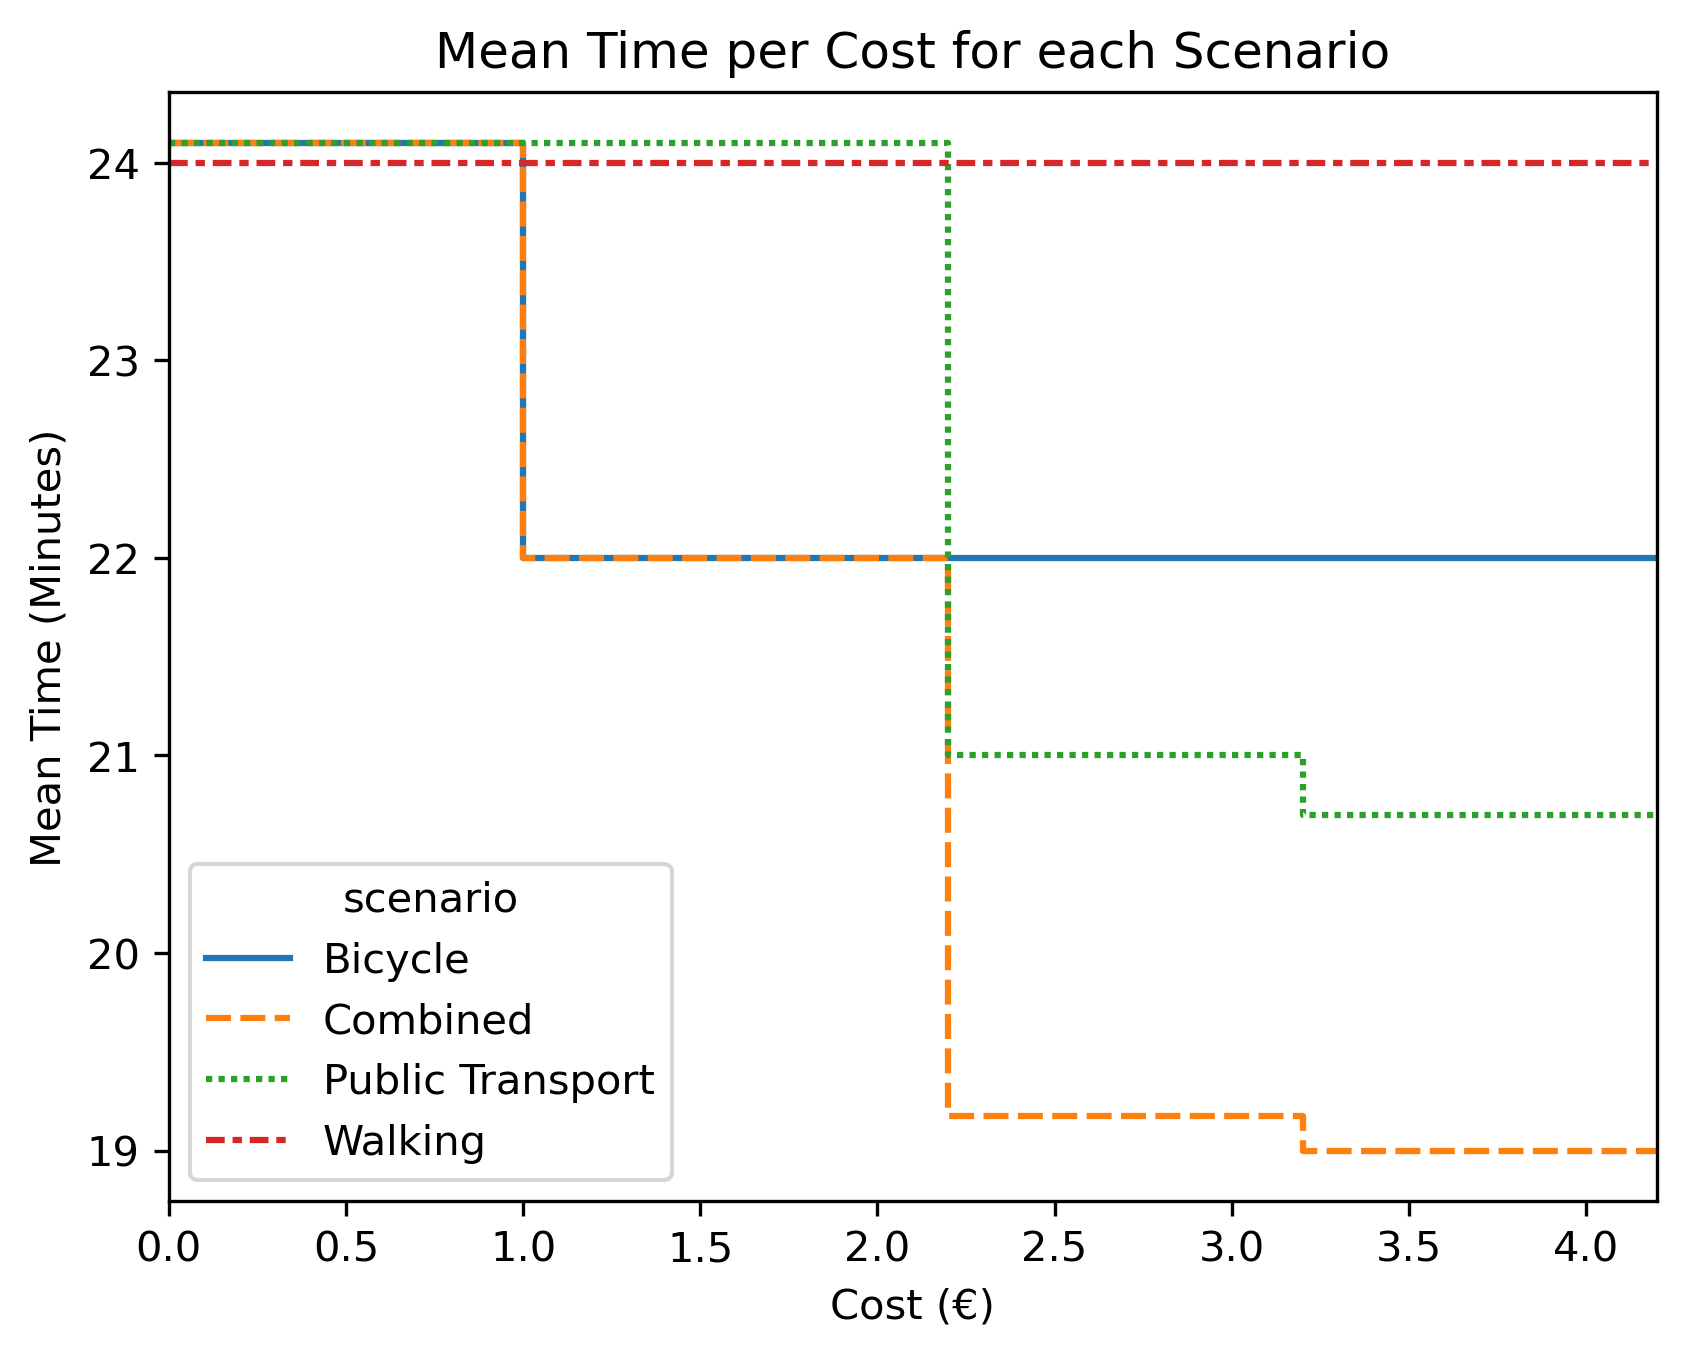
\includegraphics[width=\textwidth]{Figures/results/metric_cost/quantile_90_time_per_cost_for_each_scenario_without_car.png}
         \caption{90\% quantile time per cost for all scenarios}
         \label{fig:90_quantile_time_per_cost}
     \end{subfigure}
        \caption{Map of Optimal X-minute City Metric per Scenario}
        \label{fig:quantile_time_per_cost}
\end{figure}
The 25\% quantile Pareto front shown in Figure \ref{fig:25_quantile_time_per_cost} only contains a single improvement at the cost of \euro{1} for scenarios containing bicycle sharing of 1 minute and 45 seconds with a cost-effectiveness of 1 minute and 45 seconds per euro.
The 75\% quantile Pareto front shown in Figure \ref{fig:75_quantile_time_per_cost} with its steps shown in Table \ref{tab:differences_in_75_quantile_pareto_front} also has a similar improvement of 1 minute and 30 seconds at the cost of \euro{1} for the bicycle scenario.
In addition to that, it also shows a smaller increase at \euro{2.20} of 1 minute for the bicycle and combined scenario and an even smaller increase at \euro{3.20} only for the combined scenarios.
\begin{table}
  \caption{Steps in 75\% Quantile Pareto Front}
  \label{tab:differences_in_75_quantile_pareto_front}
  \begin{center}
    \begin{tabular}{|l|r|r|r|r|l|}
    \hline
     Scenario & Improv. & At cost (\euro) & Cost diff (\euro) & Improv. (min/\euro) \\
     \hline
     Bicycle & 1m 30s & 1.00 & 1.00 & 1m 30s \\
     \hline
     Public transport & 1m 00s & 2.00 & 2.20 & 0m 27s \\
     \hline
    \end{tabular}
  \end{center}
\end{table}
The 90\% quantile Pareto Front shown in Figure \ref{fig:90_quantile_time_per_cost} with its steps shown in Table \ref{tab:differences_in_90_quantile_pareto_front} shows a similar pattern to the 75\% quantile Pareto front.
The significant difference is that the increase at \euro{2.20} for public transport scenarios is larger than the increase at 1 euro for bicycle scenarios.
More precisely, while bicycle sharing is more effective in decreasing the 15-minute city metric on average and for the 75\% most accessible regions, public transport is more effective than bicycle sharing for the 10\% least accessible areas.
In contrast to the other quantiles we examined the improvement of the public transport scenario is larger than that of bicycle sharing. 
However, it is still less cost-effective than the improvement in the bicycle-sharing scenario.


\begin{table}
  \caption{Steps in 90\% Quantile Pareto Front}
  \label{tab:differences_in_90_quantile_pareto_front}
  \begin{center}
    \begin{tabular}{|l|r|r|r|r|l|}
    \hline
     Scenario & Improv. & At cost (\euro) & Cost diff. (\euro) & Improv. (min/\euro) \\
     \hline
     Public transport & 3m 0s & 2.20 & 2.20 & 1m 21s \\
     \hline
     Bicycle & 2m 0s & 1.00 & 1.00 & 2m 0s \\
     \hline
     Public transport & 0m 1s & 3.20 & 1.00 & 0m 1s \\
     \hline
    \end{tabular}
  \end{center}
\end{table}


\subsection{Uncertainty in Sub-scenarios}
\label{subsec:uncertainty_subscenarios}

As some of our input data is subject to uncertainties, we need to investigate the effects of these uncertainties to establish the robustness of our results.

First, we are going to look at the average standard deviation of the optimal value for the X-minute city metric in Table \ref{tab:average_standard_deviation_of_optimal_value_for_x_minute_city_metric}, which effectively shows the standard deviation of the values from Table \ref{tab:optimal_x_minute_city_metric}.
Note that we only display the average standard deviations of the bicycle, public transport, and combined scenarios, as those are the ones with uncertainty.

\begin{table}
  \caption{Average Standard Deviation of Optimal Value for X-Minute City Metric}
  \label{tab:average_standard_deviation_of_optimal_value_for_x_minute_city_metric}
  \begin{center}
    \begin{tabular}{|l|r|r|r|r|r|r|r|}
    \hline
    Scenario & mean & min & 25\% & 50\% & 75\% & max & CV (\%) \\
    \hline
    Bicycle & 1m 10s & 0m 00s & 0m 00s & 0m 32s & 1m 43s & 13m 08s & 9.38 \\
    \hline
    Combined & 0m 56s & 0m 00s & 0m 00s & 0m 44s & 1m 31s & 6m 43s & 8.25 \\
    \hline
    Public Transport & 0m 16s & 0m 00s & 0m 00s & 0m 00s & 0m 00s & 8m 39s & 2.12 \\
    \hline
    \end{tabular}
  \end{center}
\end{table}


The mean average standard deviation is the highest for the bicycle scenario with 1 minute and 10 seconds, followed by the combined scenario with 56 seconds and the public transport scenario with 16 seconds.
We can also see that for the bicycle-related scenarios, the uncertainty does not affect the 25\% most accessible hexagons, while for public transport, the 75\% most accessible hexagons are not affected.
In addition, outliers exist with more than 10 minutes of deviation for the bicycle scenario and more than 5 minutes for the combined and public transport scenario.
Relating the standard deviation to the mean, we also calculated the Coefficient of Variation (CV) in the table, which helps to grasp the relative size of the standard deviation.
It is defined as
$$ CV = \frac{\sigma}{\mu} $$
where $\mu$ is the mean and $\sigma$ is the standard deviation.
We see that it is approximately 9\% for the bicycle scenario, 8\% for the combined scenario and 2\% for the public transport scenario.

To further investigate the effects of uncertainty on a more granular level, we plot the best and worst case distribution of the optimal X-minute city for each hexagon in Figure \ref{fig:best_and_worst_case_of_optimal_time_for_each_hexagon}.
These plots are essentially the upper and lower bounds of the graph seen in Figure \ref{fig:optimal_x_minute_city_metric}.
In addition, we have added a line at the 15-minute mark to better relate the results in the context of the 15-minute city.
The best and worst-case values are calculated using the scenarios that achieve the best and worst values X-minute city metric for a given hexagon, respectively.
\begin{figure}
  \begin{center}
    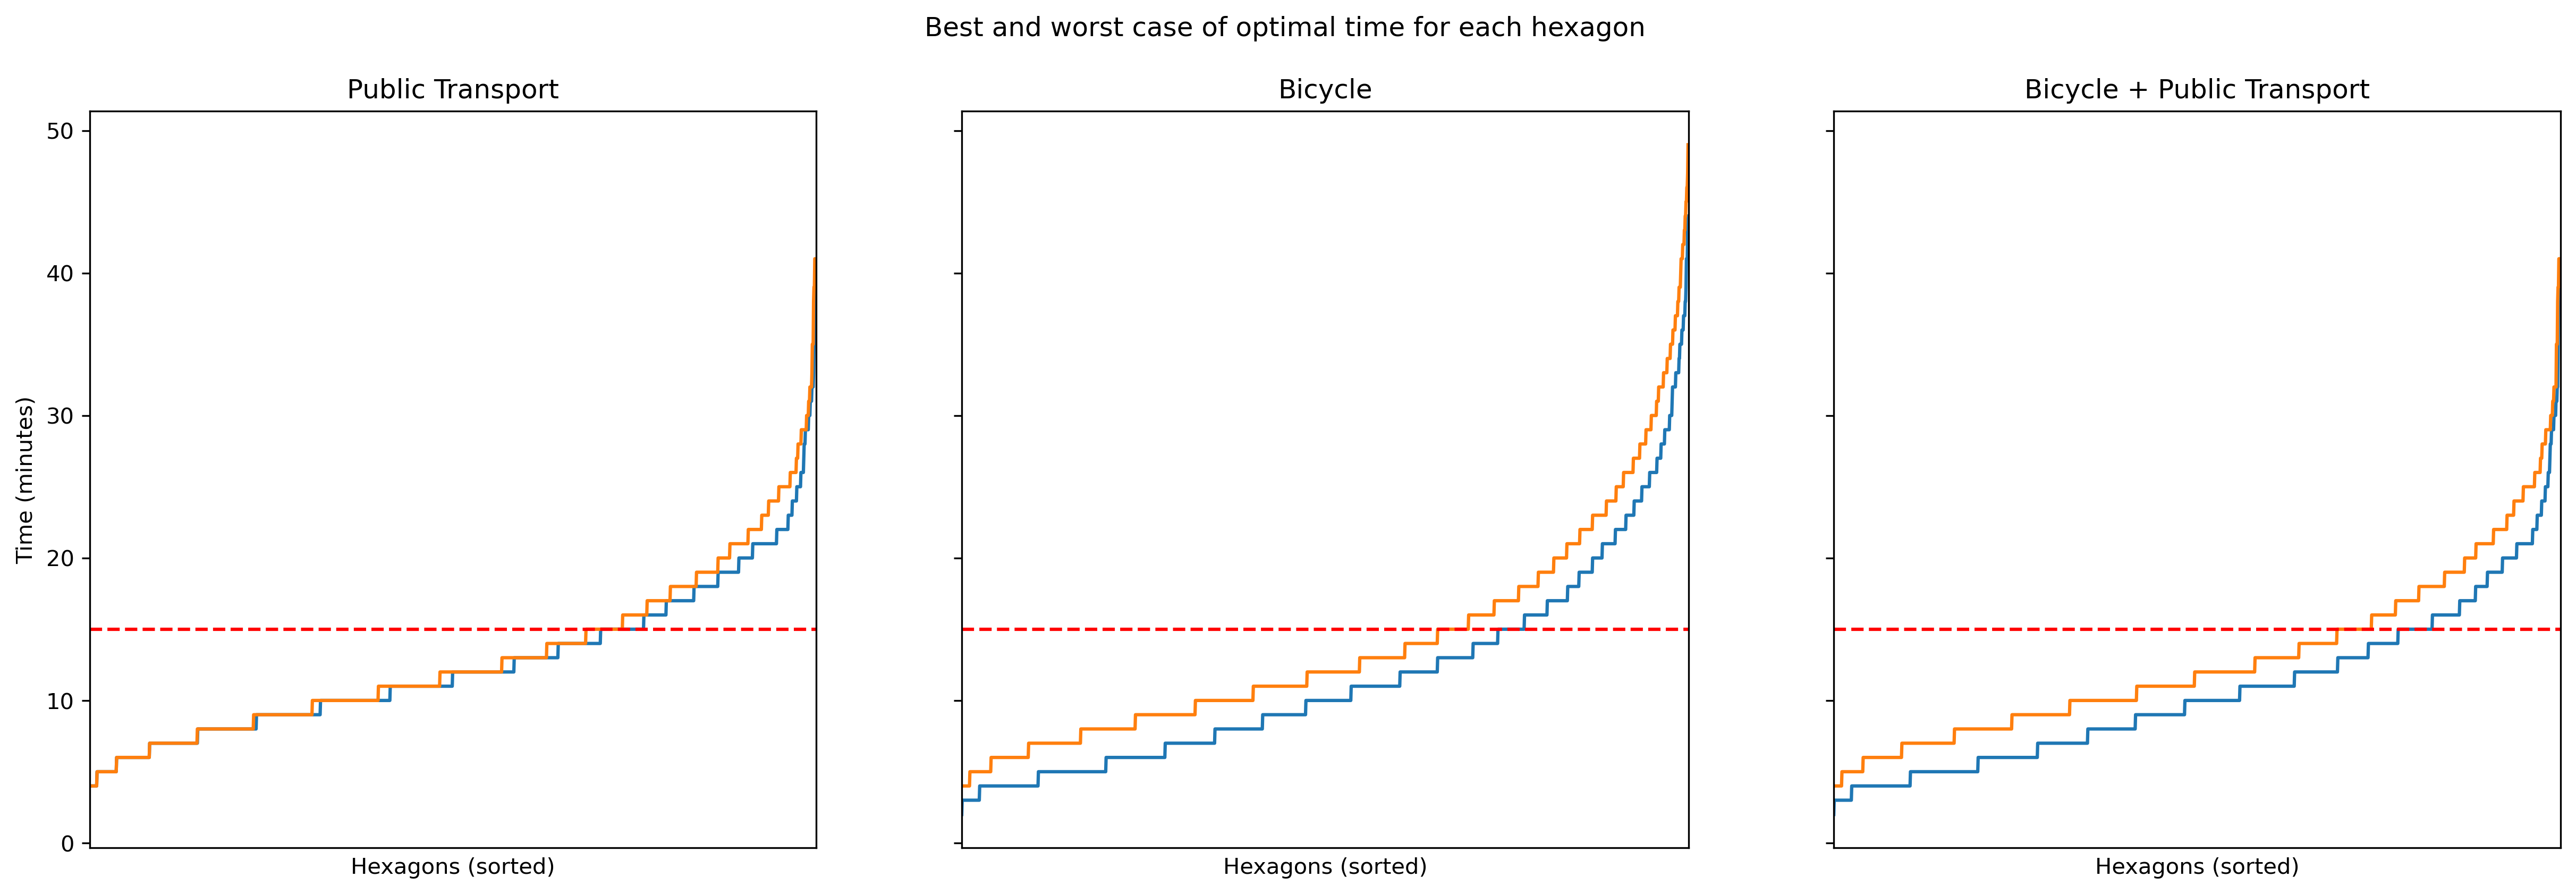
\includegraphics[width=0.95\textwidth]{Figures/results/uncertainty/optimal_best_worst_case}
  \end{center}
  \caption{Best and Worst Case of Optimal Time for each Hexagon}
  \label{fig:best_and_worst_case_of_optimal_time_for_each_hexagon}
\end{figure}
First, we see that the variation for bicycles is spread out over almost all hexagons, in comparison to public transport, where variation mostly occurs only after the 15-minute mark.
For the combined scenario, we see the expected: The variances of the public transport scenario and the bicycle scenario add up.

\subsection{Impact Of Sustainable Modes on 15-Minute Metric}
\label{subsec:impact_of_sustainable_modes_on_15_minute_metric}

To analyze the impact of sustainable modes of travel on the 15-minute city metric, we first uncover the problematic areas in which the X-minute city metric is above 15 minutes for the walking mode.
We then analyze how sustainable modes of travel can help reduce the X-minute city metric in those areas below 15 minutes.

In total, we find 552 hexagons with a walking time of more than 15 minutes to reach all POI categories, which is 30.98\% of all hexagons.
\begin{table}[h]
  \centering
  \begin{tabular}{|l|l|}
    \hline
    \textbf{Category}                                          & \textbf{Data}                \\ \hline
    Only bicycle below 15 mins                                 & 72 (13.04\%)                 \\ \hline
    Only public transport below 15 mins                        & 59 (10.69\%)                 \\ \hline
    Both bicycle and public transport below 15 mins            & 41 (7.43\%)                  \\ \hline
    Combined mode below 15 mins                                & 10 (1.81\%)                  \\ \hline
    Not reachable by sustainable modes below 15 mins           & 370 (67.03\%)                \\ \hline
    Sum           & 552 (100\%)                \\ \hline
  \end{tabular}
  \caption{Impact of Sustainable Modes on Reducing Walking Time Above 15 Minutes}
  \label{table:hexagons_with_walking_time_above_15_minutes}
\end{table}
Table \ref{table:hexagons_with_walking_time_above_15_minutes} presents the distribution of hexagons with a walking time above 15 minutes and how sustainable modes of transport can fix those hexagons.
By fixing a hexagon, we mean that residents in the hexagon cannot reach all necessities in under 15 minutes by walking, but they can make it in under 15 minutes by some other mode of transport.
A significant portion of these areas, amounting to 67.03\%, cannot be reached within 15 minutes using sustainable modes with the current state of infrastructure. 
Conversely, the data indicates that for 13.04\% of these hexagons, only bicycles can reduce travel time to under 15 minutes, while only public transport can achieve this for 10.69\% of the hexagons. 
7.43\% of hexagons are reachable with either one of bicycles or public transport, while an additional 1.81\% of hexagons are only accessible within this time frame when combining both modes. 


Next, we visualize these problematic areas spatially.
Figure \ref{fig:problematic_hexagons} displays hexagons in green where necessities can be reached within a 15-minute walk, in yellow where they are only accessible within 15 minutes using any sustainable transport, and in red where necessities are not reachable within this 15-minute timeframe.
\begin{figure}
  \begin{center}
    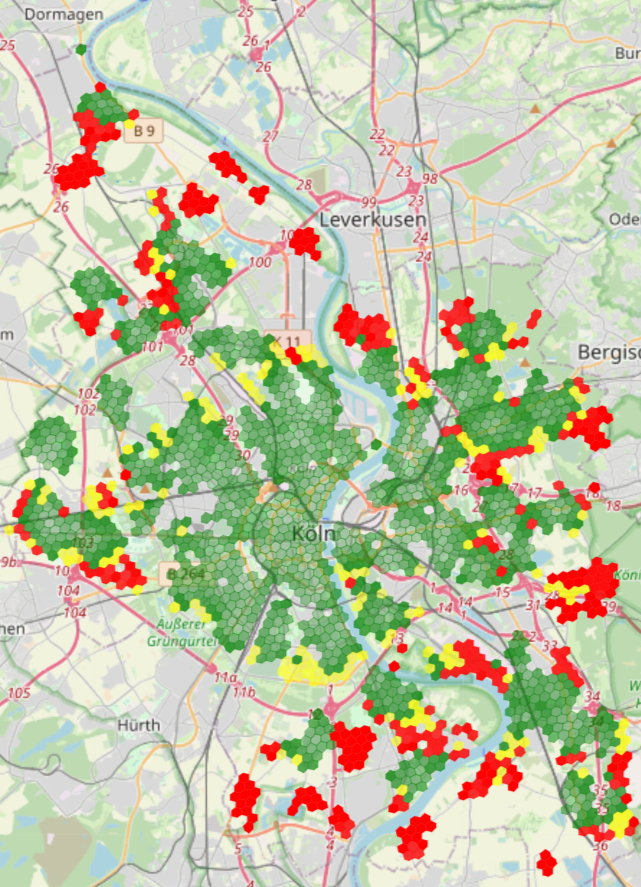
\includegraphics[width=0.50\textwidth]{Figures/results/problematic_hexagons/problematic_hexagons}
  \end{center}
  \caption{Unfixable, Fixable and Unproblematic Hexagons on a Map}
  \label{fig:problematic_hexagons}
\end{figure}
We see that in the center of Cologne, almost all hexagons qualify as 15-minute city hexagons just by walking alone.
At the city border, we see a ring of hexagons that are only valid 15-minute hexagons through additional modes of transport.
Most of the unfixable hexagons lie in the city's suburbs, often appearing in larger groups.

Next, we look at the hexagons previously colored yellow, namely those where bicycles and public transport or a combination of both can decrease the X-minute city metric below 15 minutes.
Figure \ref{fig:fixable_hexagons} illustrates hexagons representing areas that qualify as 15-minute cities via public transport in yellow, those that qualify through bicycle sharing in orange, and areas that meet the 15-minute city criteria through either mode in green.
\begin{figure}
  \begin{center}
    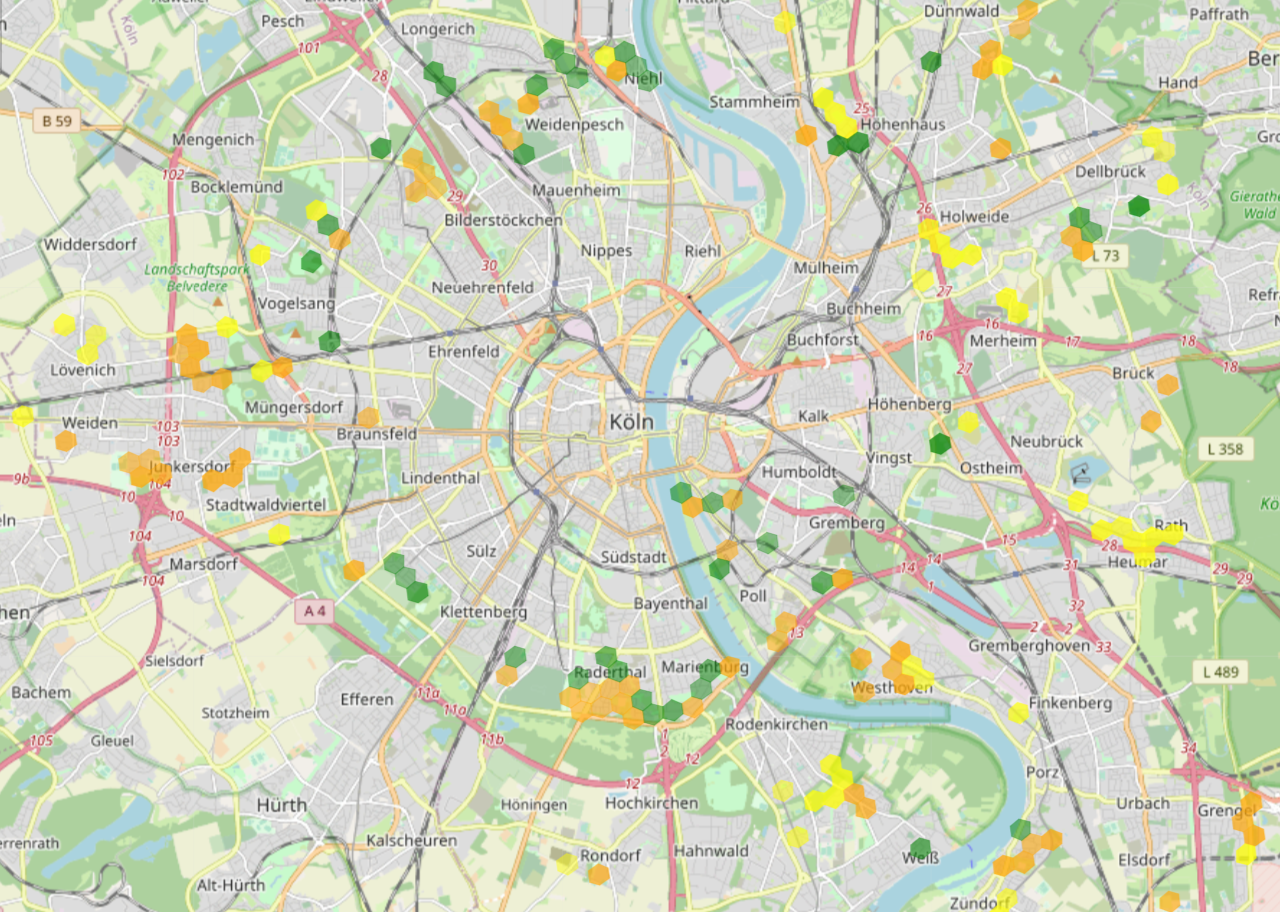
\includegraphics[width=0.70\textwidth]{Figures/results/problematic_hexagons/fixable_hexagons}
  \end{center}
  \caption{Fixable Hexagons by Mode}
  \label{fig:fixable_hexagons}
\end{figure}
The data indicates a modest trend where hexagons that achieve 15-minute city criteria solely through bicycle sharing (marked in orange) tend to be nearer to the city center than those that achieve this criterion solely via public transport (marked in yellow).

The positions of outer clusters of fixable hexagons correlate directly with the locations of bicycles and public transport stops.
Figure \ref{fig:fixable_hexagons_examples} shows four zoomed-in excerpts from Figure \ref{fig:fixable_hexagons}, where we have added the location of public transport stops and bicycles.
\begin{figure}
     \centering
     \begin{subfigure}[b]{0.45\textwidth}
         \centering
         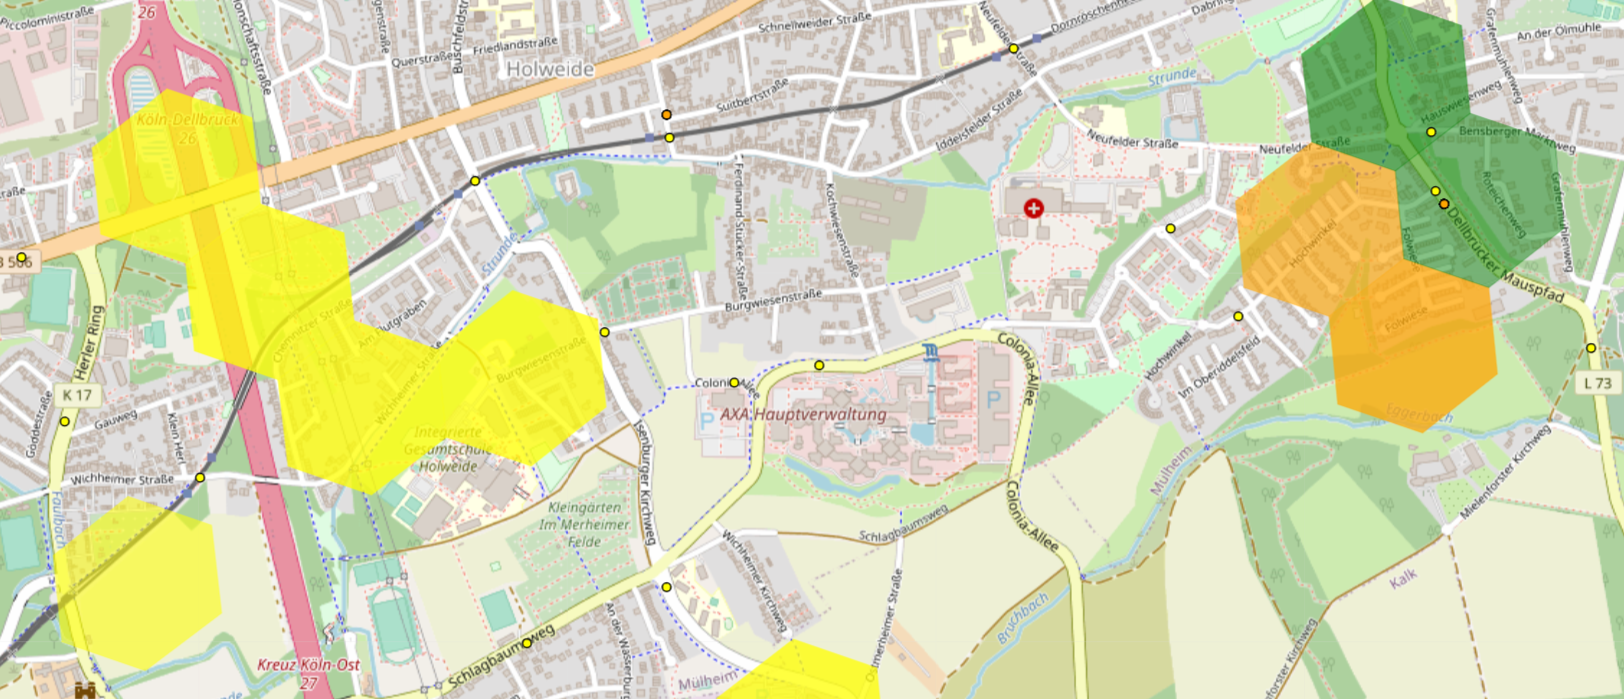
\includegraphics[width=\textwidth]{Figures/results/problematic_hexagons/example_1.png}
     \end{subfigure}
     \hfill
     \begin{subfigure}[b]{0.45\textwidth}
         \centering
         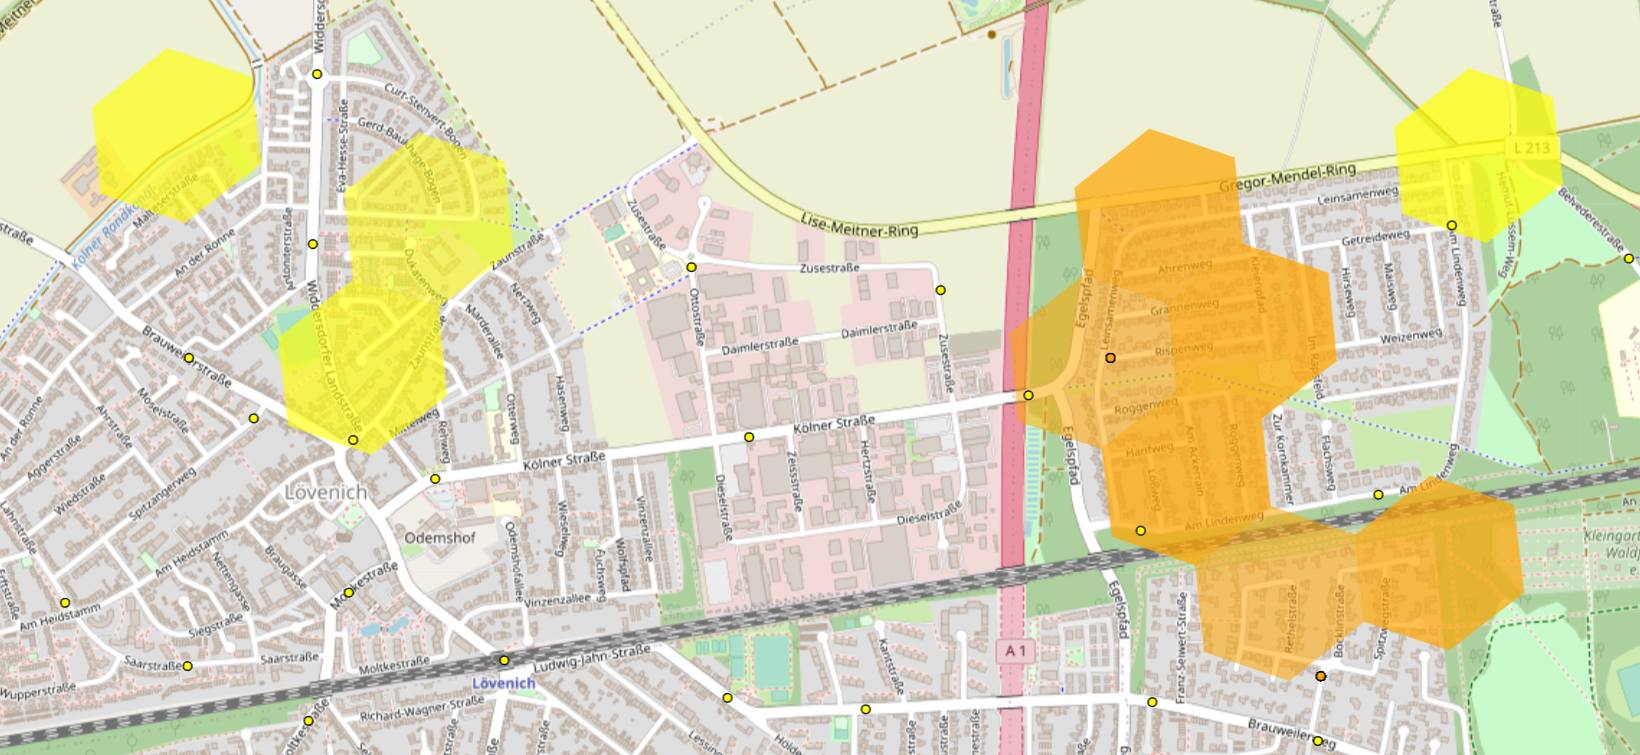
\includegraphics[width=\textwidth]{Figures/results/problematic_hexagons/example_2.png}
     \end{subfigure}
     \hfill
     \begin{subfigure}[b]{0.45\textwidth}
         \centering
         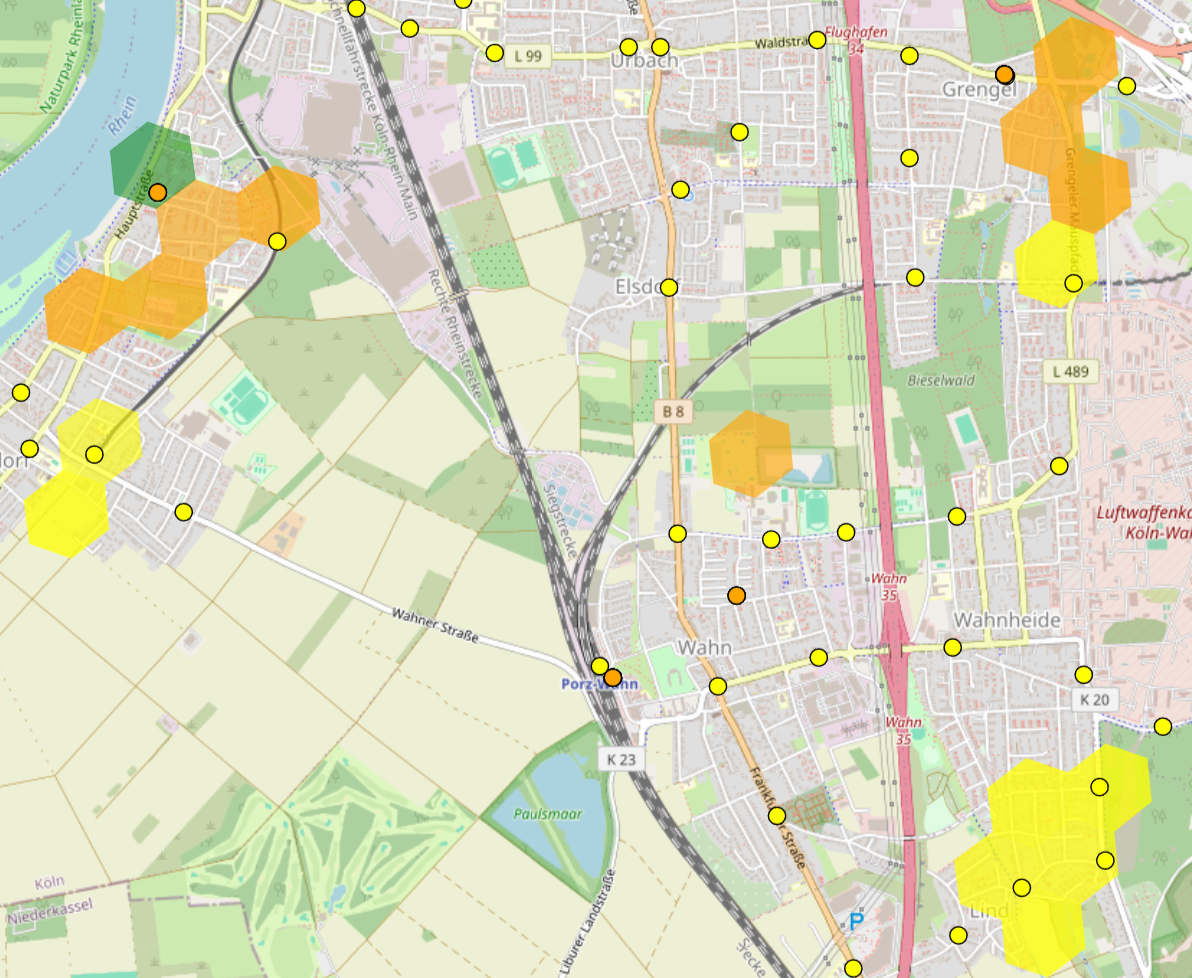
\includegraphics[width=\textwidth]{Figures/results/problematic_hexagons/example_3.png}
     \end{subfigure}
     \hfill
     \begin{subfigure}[b]{0.45\textwidth}
         \centering
         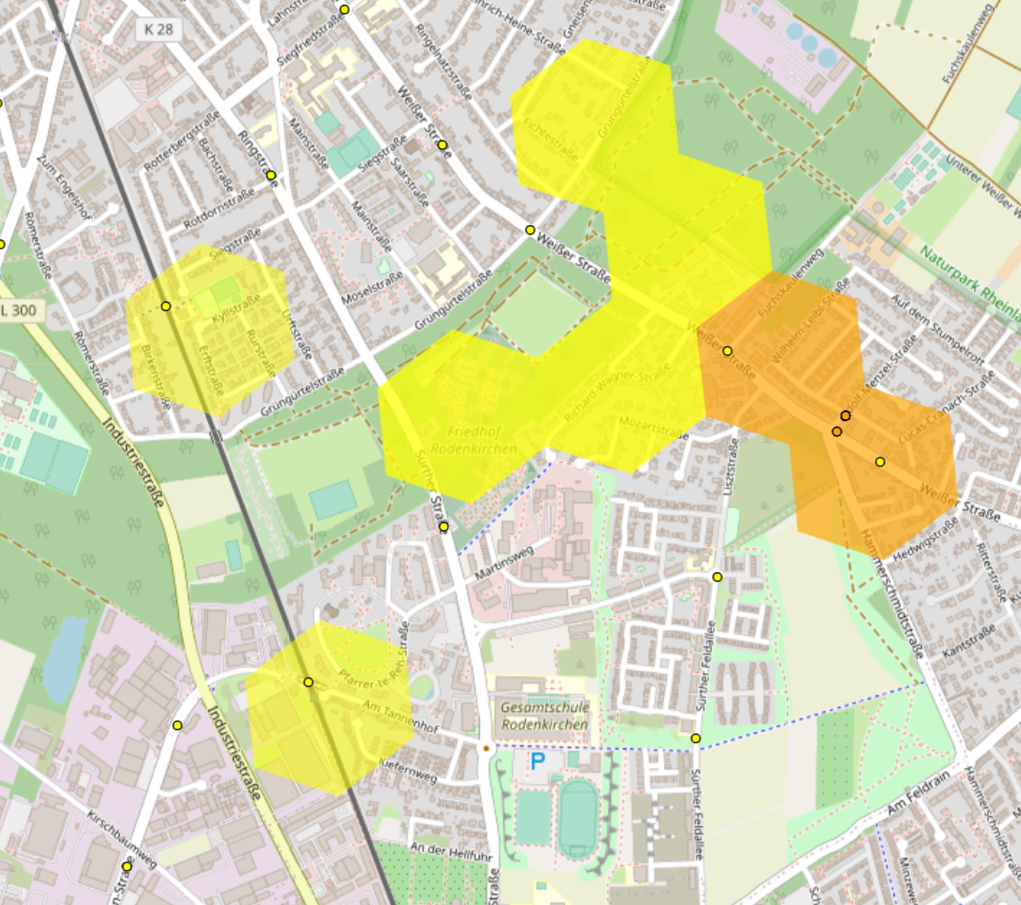
\includegraphics[width=\textwidth]{Figures/results/problematic_hexagons/example_4.png}
     \end{subfigure}
     \caption{Examples of Fixable Hexagons}
        \label{fig:fixable_hexagons_examples}
\end{figure}
Public transport stops are visualized as yellow circles, while bicycles are visualized as orange circles.
We notice that hexagons fixed by bicycle sharing are always near bicycles.
In the same way, hexagons fixed by public transport are always close to public transport stops. 
However, being close to bike stations seems to have a more significant effect than being near public transport stops.

Figure \ref{fig:only_unfixable_hexagons} shows all hexagons that are not 15-minute hexagons by any sustainable mode of transport.
Figure \ref{fig:unfixable_with_bicycles} and \ref{fig:unfixable_with_stops} show the same map but with additional bicycle locations and public transport stop locations, respectively.
\begin{figure}
     \centering
     \begin{subfigure}[b]{0.30\textwidth}
         \centering
         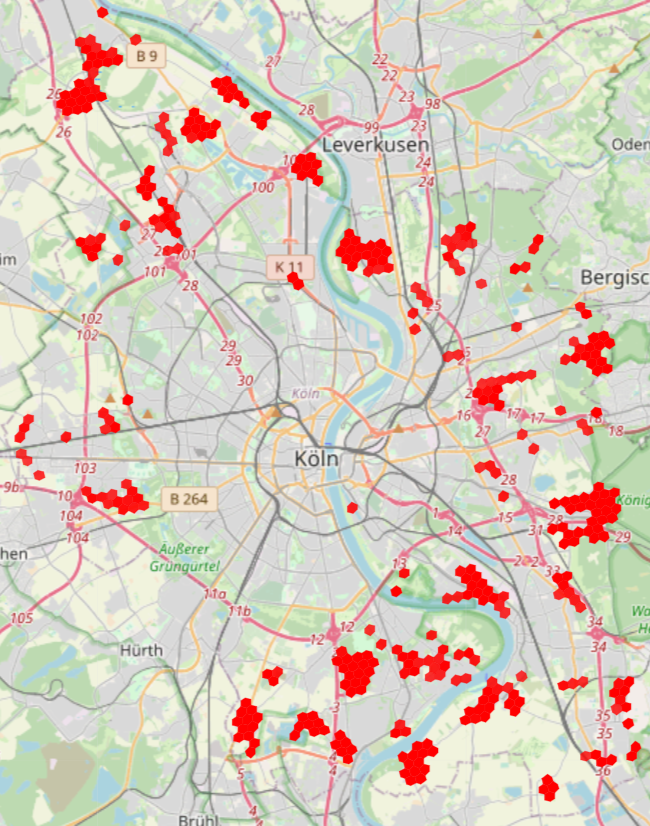
\includegraphics[width=\textwidth]{Figures/results/problematic_hexagons/unfixable.png}
         \caption{Only Unfixable Hexagons}
         \label{fig:only_unfixable_hexagons}
     \end{subfigure}
     \hfill
     \begin{subfigure}[b]{0.30\textwidth}
         \centering
         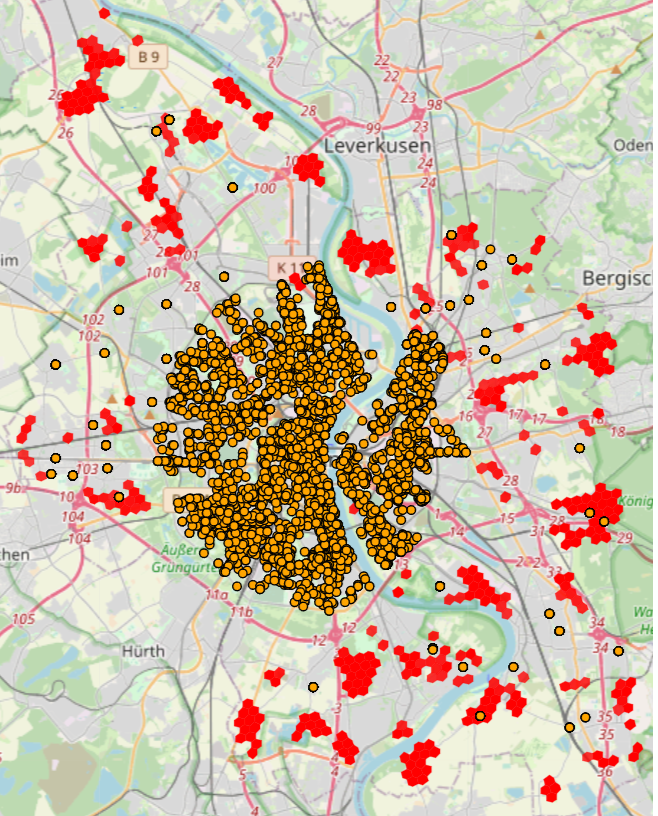
\includegraphics[width=\textwidth]{Figures/results/problematic_hexagons/unfixable_with_bicycles.png}
         \caption{With All Bicycle Locations}
         \label{fig:unfixable_with_bicycles}
     \end{subfigure}
     \hfill
     \begin{subfigure}[b]{0.30\textwidth}
         \centering
         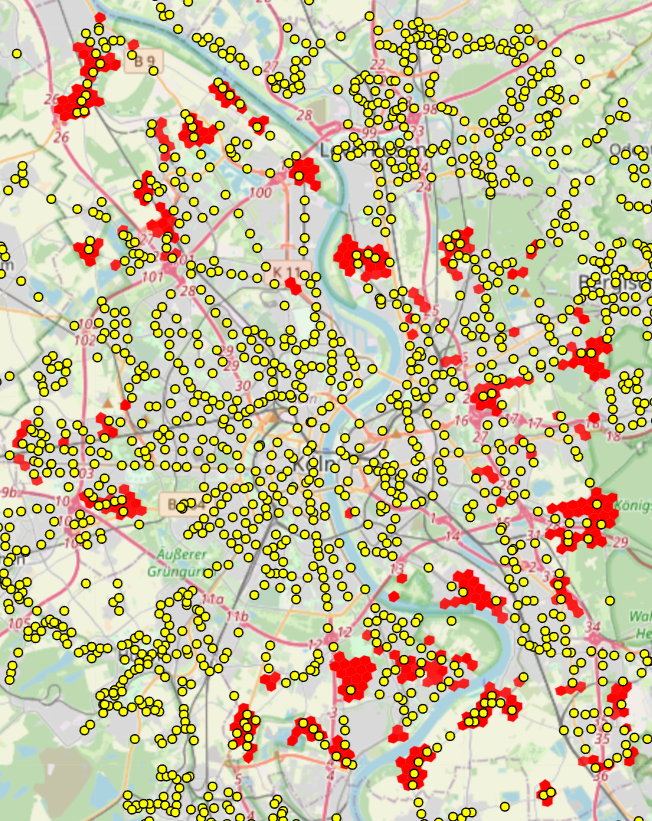
\includegraphics[width=\textwidth]{Figures/results/problematic_hexagons/unfixable_with_stops.png}
         \caption{With Public Transport Stops}
         \label{fig:unfixable_with_stops}
     \end{subfigure}
     \hfill
     \caption{Unfixable Hexagons}
     \label{fig:unfixable_hexagons}
\end{figure}
We can observe that the unfixable hexagons mostly do not contain any bicycles and have a larger distance to the nearest bicycle.
The same cannot be said for public transport stops, as public transport stops are often directly inside the unfixable hexagons.

Figure \ref{fig:combined_hexagons} shows all hexagons that only become 15-minute city hexagons in the combined scenario when public transport and bicycle sharing are used simultaneously.
As already seen in Table \ref{table:hexagons_with_walking_time_above_15_minutes}, this only concerns less than 2\% of all hexagons that are not already 15-minute city hexagons through walking alone.
More than half of those (7 out of 10) are located in the southern district of Weiß.
\begin{figure}
  \begin{center}
    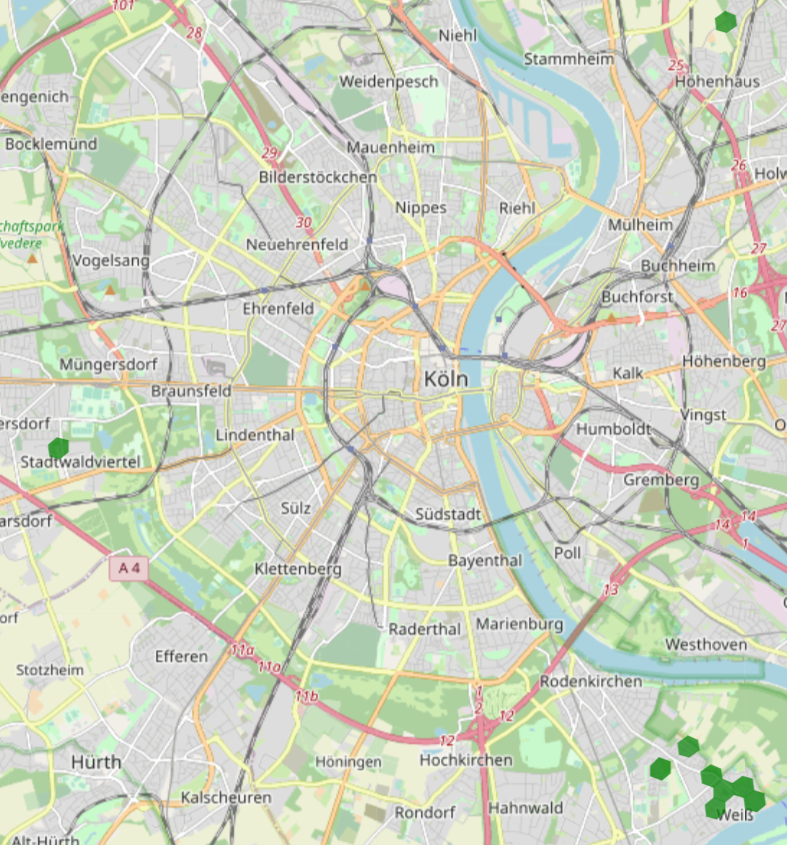
\includegraphics[width=0.50\textwidth]{Figures/results/problematic_hexagons/combined_hexagons}
  \end{center}
  \caption{Hexagons Fixable by Combined Mode}
  \label{fig:combined_hexagons}
\end{figure}


\subsection{Monthly Costs Per Scenario And Hexagon}
\label{sec:monthly_costs}
A prevalent measure to incentivize sustainable modes of transport is monthly tickets or subscriptions.
To measure whether the costs of these subscriptions are worth it, we will calculate the monthly cost incurred by the trips to all necessities.
To do so, we first collect how often people visit each POI category we defined earlier and visualize this data in Table \ref{tab:monthly_visits}.
The derivation of these numbers, as well as the sources, can be found in Appendix \ref{app:monthly_visits_per_category}.

To understand and compare the usual monthly costs caused by traveling with different modes of transport, we first establish two time-based benchmarks to compare the cost incurred.
The first benchmark focuses on the costs incurred when reaching the nearest POI of a given category within a 15-minute timeframe. 
The second benchmark assesses the costs for a similar journey but within a more constrained 10-minute limit.
However, to compare these costs, a journey in that time has to be possible, which is not always the case.

\begin{table}
  \caption{Number of Monthly Visits per Category}
  \label{tab:monthly_visits}
  \begin{center}
    \begin{tabular}[c]{l|l}
      category & monthly visits \\
      \hline
      groceries & 12 \\
      education & 20 \\
      health & 0.42 \\
      banks & 9 \\
      parks & 2.4 \\
      sustenance & 6.12 \\
      shops & 4 \\
      \hline
    \end{tabular}
  \end{center}
\end{table}

Therefore, we show how often a journey is possible within the given timeframe in Figure \ref{fig:percentage_inf_x}.
In the 10-minute benchmark, the combined scenario of bicycle sharing and public transport fails the least, with a maximum of 36\% for the bank category, followed by public transport and bicycle sharing.
In the 15-minute benchmark, bicycle sharing and public transport perform almost equally well, while in the 10-minute benchmark, bicycle sharing performs better than public transport.
Category-wise, banks seem to be the least accessible category, followed by parks and health.
Sustenance, education, grocery, and shops all seem similarly accessible.

\begin{figure}
  \centering
  \begin{subfigure}[b]{0.45\textwidth}
    \centering
    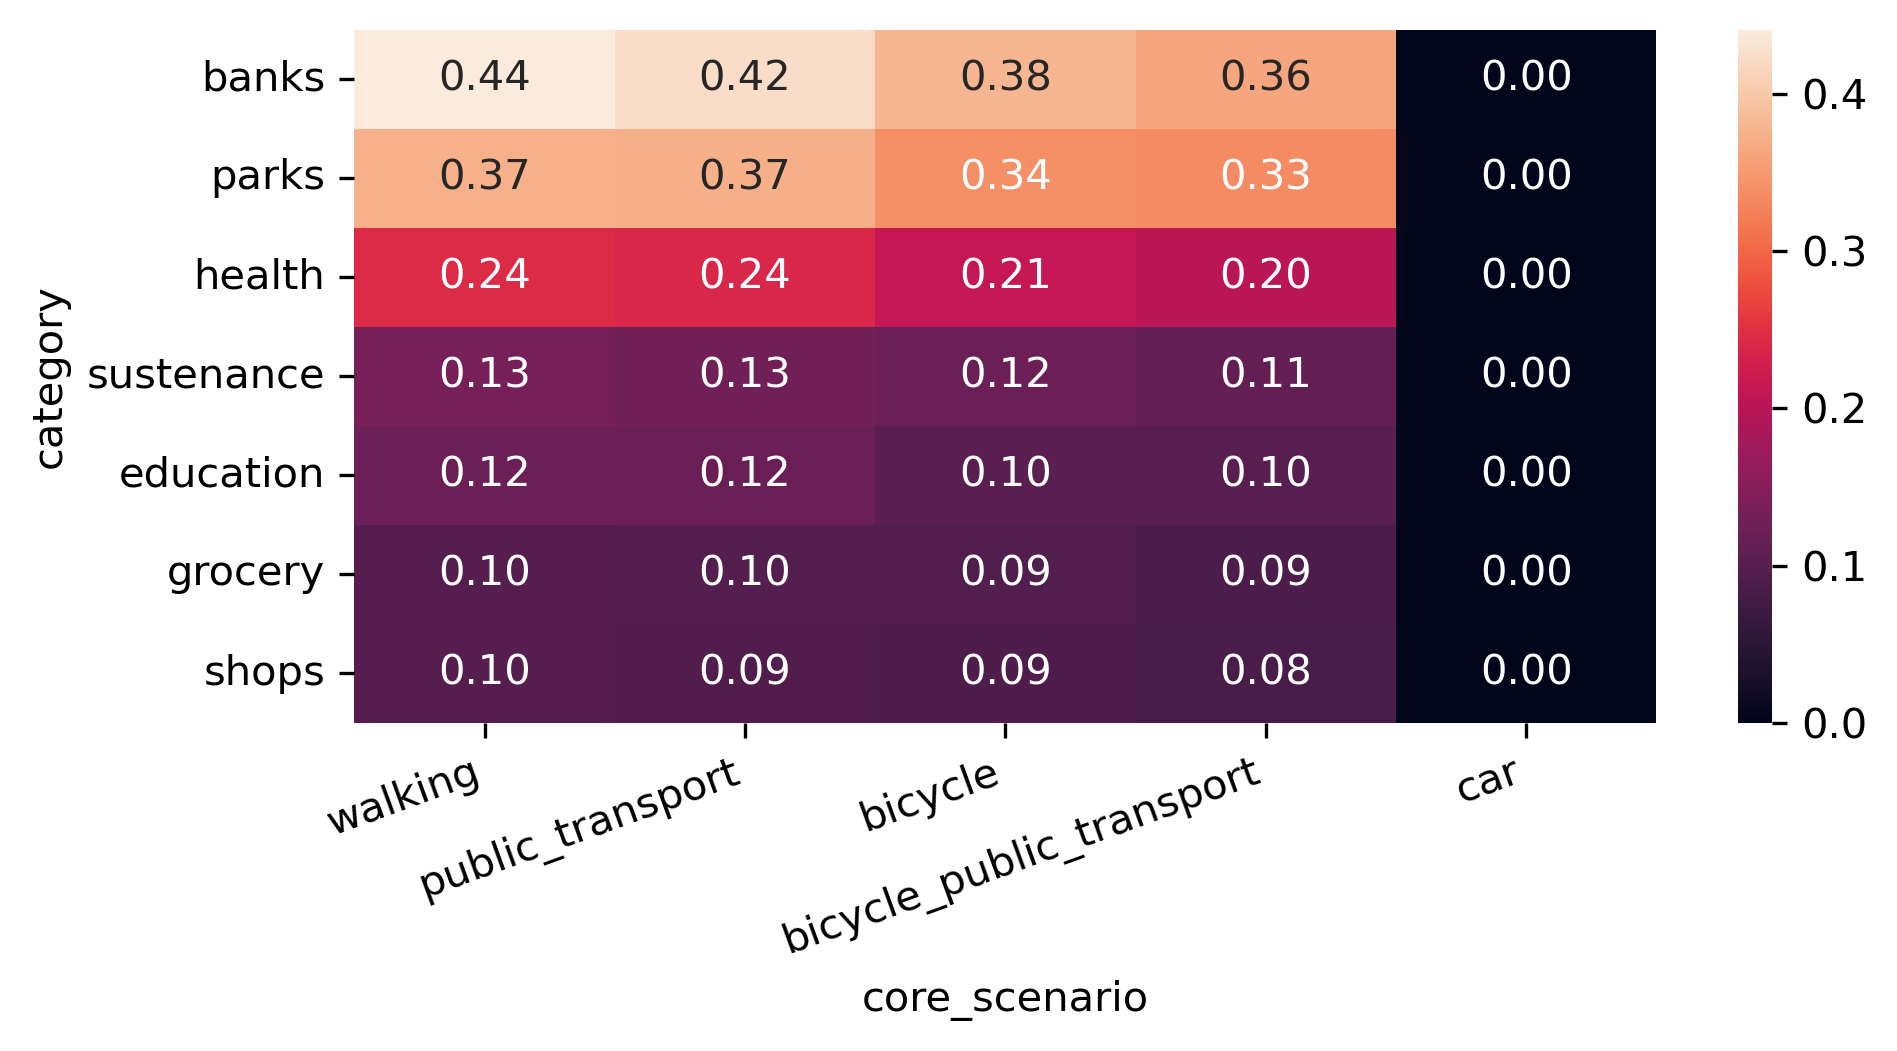
\includegraphics[width=\textwidth]{Figures/results/monthly_costs/percentage_inf_10.png}
    \caption{10 Minutes}
    \label{fig:percentage_inf_10}
  \end{subfigure}
  \hfill
  \begin{subfigure}[b]{0.45\textwidth}
    \centering
    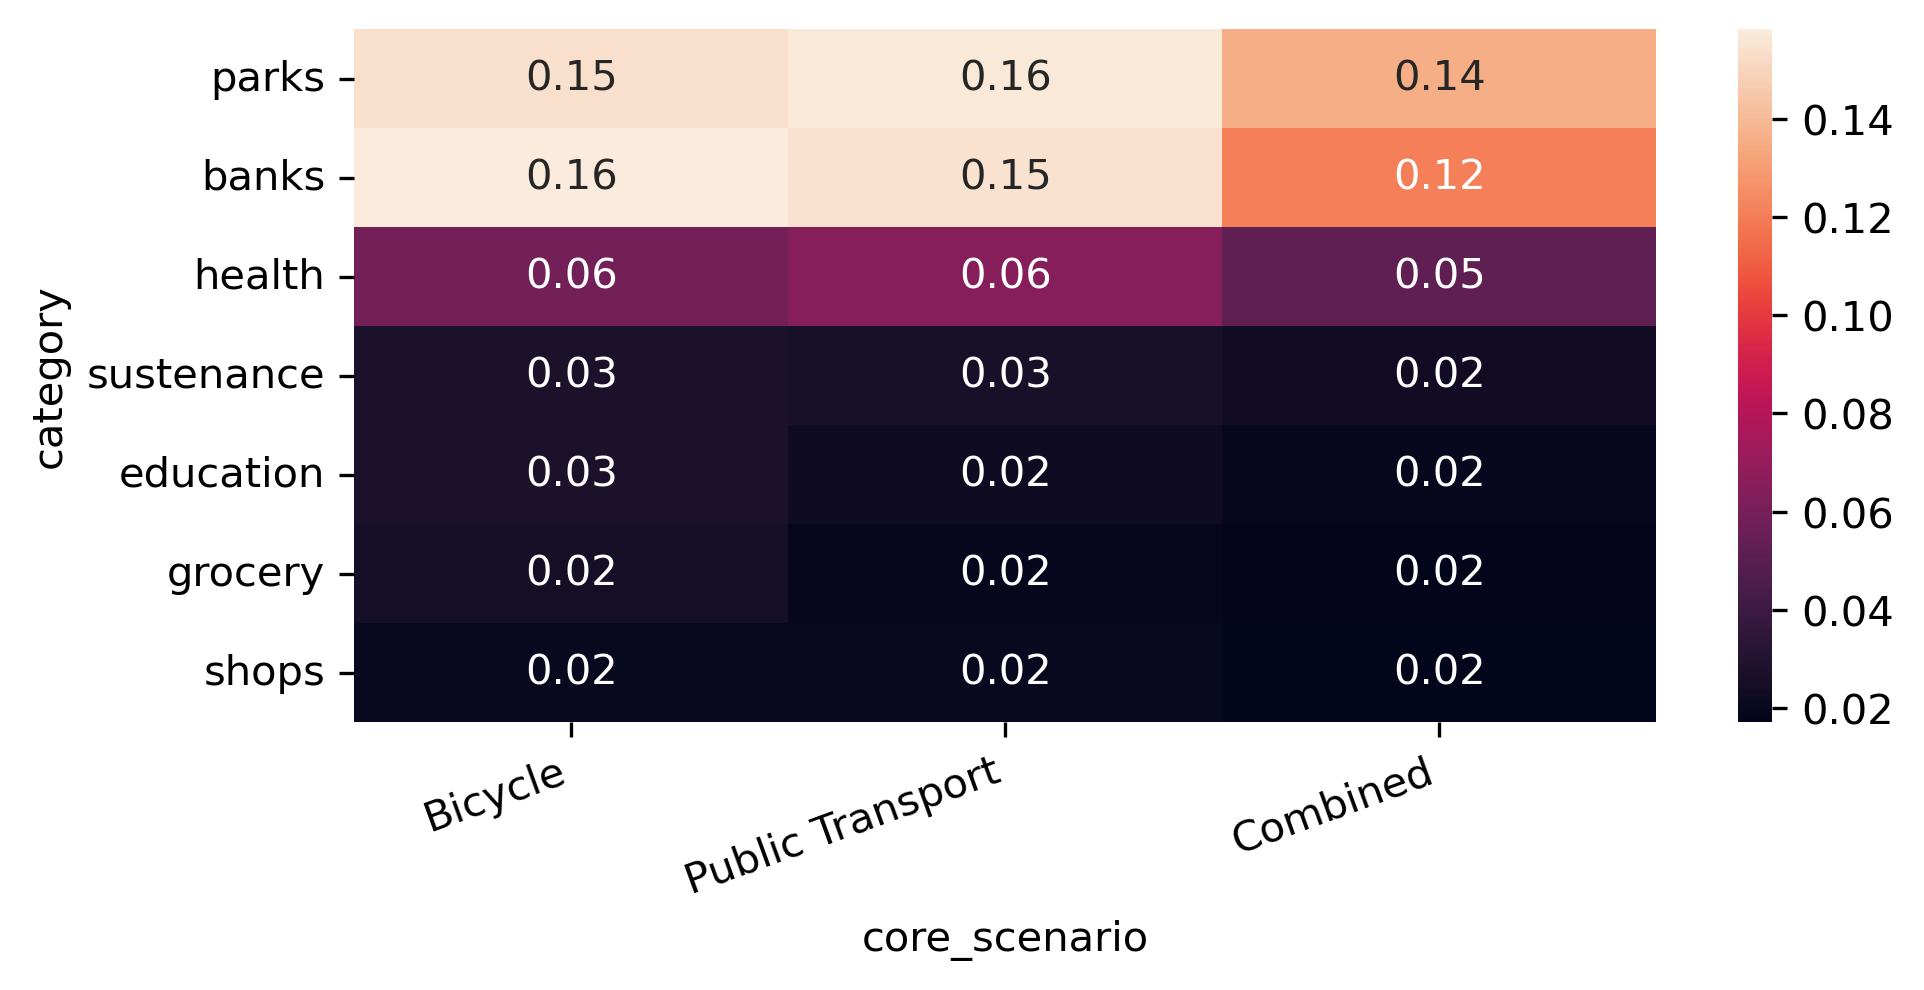
\includegraphics[width=\textwidth]{Figures/results/monthly_costs/percentage_inf_15.png}
    \caption{15 Minutes}
    \label{fig:percentage_inf_15}
  \end{subfigure}
  \caption{Impossible Sub-X-Minute Journeys for each Hexagon and Scenario}
  \label{fig:percentage_inf_x}
\end{figure}

As seen in the previously discussed Figure \ref{fig:percentage_inf_x}, the number of impossible journeys differs across scenarios.
This, again, makes it hard to compare the costs across scenarios.
Therefore, we will only look at hexagons and category combinations where a journey is possible within the given timeframe for all scenarios with sustainable transport modes.
In addition, we also filter out hexagon category combinations where the cost is zero, i.e. where walking suffices, as those are not interesting for our cost analysis.

\begin{table}
  \caption{Monthly costs per scenario (<15 minutes)}
  \label{tab:monthly_costs_per_scenario_15}
  \begin{center}
    \begin{tabular}{lrrrrrrr}
     & mean & std & min & 25\% & 50\% & 75\% & max \\
    Scenario &  &  &  &  &  &  &  \\
    Bicycle & 5.79 & 5.95 & 0.42 & 0.42 & 4.00 & 9.00 & 29.00 \\
    Combined & 5.79 & 5.95 & 0.42 & 0.42 & 4.00 & 9.00 & 29.00 \\
    Public Transport & 12.93 & 13.26 & 0.93 & 0.93 & 8.80 & 19.80 & 63.80 \\
    \end{tabular}
  \end{center}
\end{table}


\begin{table}
  \caption{Monthly costs per scenario (<10 minutes)}
  \label{tab:monthly_costs_per_scenario_10}
  \begin{center}
    \begin{tabular}{lrrrrrrr}
     & mean & std & min & 25\% & 50\% & 75\% & max \\
    Scenario &  &  &  &  &  &  &  \\
    Bicycle & 10.49 & 7.72 & 0.42 & 2.42 & 9.00 & 20.00 & 24.54 \\
    Combined & 10.49 & 7.72 & 0.42 & 2.42 & 9.00 & 20.00 & 24.54 \\
    Public Transport & 23.08 & 16.98 & 0.93 & 5.32 & 19.80 & 44.00 & 53.98 \\
    \end{tabular}
  \end{center}
\end{table}

Table \ref{tab:monthly_costs_per_scenario_15} shows the average monthly costs to reach all categories within 15 minutes for each scenario, and Table \ref{tab:monthly_costs_per_scenario_10} shows the same for 10 minutes.
As we can see, the total cost averages at \euro{5.80} for the bicycle and combined scenario and \euro{12.90} for the public transport scenario in the 15-minute benchmark.
The cost reaches a maximum of \euro{29} for the bicycle and combined scenario and \euro{63.8} for the public transport scenario, while the 25\% most expensive hexagons require residents to pay at least \euro{9} for the bicycle and combined scenario and \euro{19.80} for the public transport scenario.
Note that the bicycle and combined scenario always have the same cost, showing that it is not worth using public transport, when bicycle sharing is available in those hexagons.
In the 10-minute benchmark, the average cost is \euro{10.5} for the bicycle and combined scenario and \euro{23.1} for the public transport scenario.
Here, the cost reaches a maximum of \euro{24.54} for the bicycle and combined scenario and \euro{53.98} for the public transport scenario, while the 25\% most expensive hexagons require residents to pay at least \euro{20} for the bicycle and combined scenario and \euro{44} for the public transport scenario.

\begin{table}
  \caption{Monthly costs for cars}
  \label{tab:monthly_costs_for_cars}
  \begin{center}
    \begin{tabular}{lrrrrrrr}
     & mean & std & min & 25\% & 50\% & 75\% & max \\
    Car (15 Minutes) & 1.79 & 1.69 & 0.00 & 0.46 & 1.71 & 1.79 & 7.00 \\
    Car (10 Minutes) & 2.87 & 2.89 & 0.00 & 0.46 & 1.79 & 3.91 & 10.88 \\
    \end{tabular}
  \end{center}
\end{table}

Next, we will also look at the monthly costs for the car scenario in the same hexagons we considered previously in Figure \ref{tab:monthly_costs_for_cars}.
This allows us to compare the cost of cars with other modes of transport.
We see that the average cost is \euro{1.79} for the 15-minute benchmark and \euro{2.87} for the 10-minute benchmark, which in both cases is less than a third of the cheapest sustainable mode of transport.
However, we need to take into account that the cost of \euro{0.19}/min tries to capture fuel costs, repair costs, insurance, and tax, but not acquisition costs.

\clearpage
\section{Discussion}
\label{sec:discussion}

\subsection{Interpretation of Results}

\subsubsection{Runtime Observations}
We've shown that our method is applicable to a large city like Cologne, running in a reasonable amount of time on consumer hardware.
While the memory footprints may exceed 32 GB, using swap memory did not degrade the runtime beyond a reasonable amount.
We therefore conclude that our method is applicable to cities of similar size.
Also, because our method is parallelizable, we expect that it will scale well when using more powerful hardware.

\subsubsection{Public Transport Effectiveness}
Our findings indicate that public transport effectively enhances accessibility, particularly in remote, low-POI-density suburban areas near high-frequency transport lines. 
However, it is costlier compared to bicycle sharing.
We summarize our findings for public transport effectiveness in the following inferences:
\begin{enumerate}
  \renewcommand{\labelenumi}{I\theenumi.}
  \item Public transport improves accessibility \label{item:pt_improves_accessibility}
  \item Public transport is more effective in remote areas \label{item:pt_effective_in_remote_areas}
  \item Public transport is more effective in areas with low accessibility \label{item:pt_effective_in_areas_with_low_accessibility}
  \item Public transport is costlier than bicycle sharing \label{item:pt_costlier_than_bicycle_sharing}
\end{enumerate}
We will now reiterate our results and show how they support the inferences above.

In Figure \ref{fig:mean_time_per_cost} we can clearly see that when users are able to afford a short public transport trip (cost of 2.20), their accessibility to POIs increases (I\ref{item:pt_improves_accessibility}).

% pt for areas of low accessiblity 
The improvement seen by adding public transport mainly comes from areas with low accessibility as seen in Table \ref{tab:optimal_x_minute_city_metric} and Figure \ref{fig:optimal_x_minute_city_metric} (I\ref{item:pt_effective_in_areas_with_low_accessibility}).
These areas, or hexagons, are likely far from POIs, and we suspect that public transport helps by covering these longer distances. 
However, in areas where it's already easy to get to these places, adding public transport might not make a big difference. 
This is because using public transport often involves extra steps: walking to the bus or train stop and waiting for it to arrive. 
How much this extra time matters depends on how long the whole trip is.
For short trips, the time spent getting to and waiting for public transport could be a large part of the travel time, making it less useful. 
But for longer trips, especially in the areas that were hard to reach before, this extra time is a smaller part of the journey. 
This makes public transport more beneficial for these longer trips. 

% pt actually better than bicycle for 20% worst
In Figure \ref{fig:optimal_x_minute_city_metric} we see the full distribution of the optimal X-minute city metric for each scenario.
Notably, while public transport is worse than bicycle sharing for the 80\% most accessible hexagons it shows a distinct advantage over bicycle sharing beyond the 80\% quantile, facilitating faster access in less accessible areas (I\ref{item:pt_effective_in_areas_with_low_accessibility}).
The reason for this change in effectiveness between public transport and bicycle sharing is most likely linked to how bicycle sharing is set up in Cologne. 
With the majority of bicycles available in the city center's "Flex-Zone", suburban areas have fewer bicycles as they can only be found at stations.
Consequently, the least accessible hexagons, typically situated in suburban regions, experience low to no availability of bicycles, which explains the superiority of public transport in these areas. 

% rath/neumar is reachable better by pt
Inferences \ref{item:pt_effective_in_areas_with_low_accessibility} and \ref{item:pt_effective_in_remote_areas} are supported by comparing the optimal X-minute city metric spatially between public transport and bicycle sharing, as seen in Figure \ref{fig:bicycle_optimal_map} and \ref{fig:public_transport_optimal_map}.
We see the district of Rath/Neumar in the east, which shows low accessibility in general.
However, we can clearly see that public transport has an advantage over bicycle sharing in this remote area.

% pt in hexagons with walking time above 15 minutes
When looking at Table \ref{table:hexagons_with_walking_time_above_15_minutes} we see that public transport is able to make 10\% of hexagons that are not valid in terms of the 15-minute city by walking alone, valid (\ref{item:pt_improves_accessibility}).
In addition, when looking at the spatial distribution of those hexagons in Figure \ref{fig:fixable_hexagons}, we see that the yellow hexagons, which are those that, become valid in terms of the 15-minute city only through public transport, are mostly located outside the city in remote areas (I\ref{item:pt_effective_in_remote_areas}).

% pt only better at 90% pareto front
In addition, when investigating the cost and X-minute city metric Pareto fronts in Figure \ref{fig:quantile_time_per_cost}, we see that public transport is only able to yield larger improvements than bicycle sharing when considering only the 10\% worst accessible hexagons (I\ref{item:pt_effective_in_areas_with_low_accessibility}).

% cost stuff
Table \ref{tab:required_cost} and Figure \ref{fig:maximum_required_cost_for_x_minute_city} show that public transport's advantage at the least accessible hexagons comes at a cost (I\ref{item:pt_costlier_than_bicycle_sharing}).
As soon, as the benefits of public transport manifest, the cost also increases to \euro{2.20}, which is obvious as public transport rides are always charged.
We can see, however, that is really rarely necessary to travel more than four stops, as the cost for that (\euro{3.20}) is only reached at the very end. 
The three- or four-step increases to the cost of \euro{2.20} and \euro{3.20} can be explained by the different sub-scenarios.
In some scenarios it might be only beneficial to use public transport later.

Looking at Figure \ref{fig:maximum_required_cost_for_x_minute_city} also clearly reveals the spatial usage pattern of public transport.
As already conjectured previously, we see that mostly public transport is used in remote locations outside the city, that we know have lower accessibility in general (I\ref{item:pt_effective_in_remote_areas} \& I\ref{item:pt_effective_in_areas_with_low_accessibility}).

The single hexagons inside the cities seen in Figure \ref{fig:maximum_required_cost_for_x_minute_city} are most likely located very close to a public transport stop, enabling to use the public transport system without any loss of time.
Inside the city it seems to only be beneficial to use the public transport system to reach necessities when living near a stop.
However, outside the city the larger groups of hexagons indicate that using the public transport system is often faster than walking to the necessities, even though walking to the next stop requires some time (I\ref{item:pt_effective_in_remote_areas}).
This may be, because the density of the POIs is lower outside the city.

% comparison of usefulness of short and long trips (not assigned to inference)
With the help of the cost and X-minute city metric Pareto fronts, we are able to evaluate the usefulness and cost-efficiency of short trips (those that travel no more than 4 stops) and long trips (those that travel more than 4 stops).
Figure \ref{fig:mean_time_per_cost} and Table \ref{tab:differences_in_mean_pareto_front} show that the improvement caused by the short trip tickets is on average 1.28 minutes, compared to the 0.074 minutes of long trip tickets, and therefore almost 20 times larger.
Different from what we previously inferred (I\ref{item:pt_effective_in_remote_areas}), it seems that the most effective and cost-efficient use of public transport consists of short trips.
However, we should note that just because it does not bring as much value to travel more than four stops, this does not mean that trips associated with four stops or fewer are short.
Especially in suburban areas, where public transport stops are more sparse than in the city center, it might very well be that trips with four stops or fewer still travel multiple kilometers.
When investigating the 25\% quantile and 75\% quantile Pareto fronts in Figure \ref{fig:quantile_time_per_cost}, there is no benefit of long distance tickets displayed.
Only when investigating the 90\% quantile Pareto front, the benefit is visible.
This indicates that long distance trips are only used for the least accessible hexagons, which are located outside the city \ref{item:pt_effective_in_remote_areas}.

% Rath/Neumar
In Figure \ref{fig:public_transport_optimal_map} we see that while the district of Rath/Neumar shows bad accessibility for all three scenarios, however, the accessibility in the public transport is better than that of walking and bicycle sharing (I\ref{item:pt_effective_in_remote_areas}).
Also, we know that the high-frequency city train line 9 runs through this region, which explains the effectiveness of public transport in this region (I\ref{item:pt_effective_in_areas_with_low_accessibility}).
It also shows us that, a high frequency public transport line from the city center to less accessible area can significantly improve accessibility.

\subsubsection{Bicycle Sharing Effectiveness}
% intro
Bicycle sharing enhances accessibility in both less and well-connected urban areas, offering cost-efficiency over public transport, with its effectiveness highly depending on bicycle allocation.
We summarize our findings for bicycle sharing effectiveness in the following inferences:

\begin{enumerate}
  \renewcommand{\labelenumi}{I\theenumi.}
  \item Bicycle sharing improves accessibility \label{item:bicycle_improves_accessibility}
  \item Bicycle sharing is able to further improve accessibility in already well-connected areas \label{item:bicycle_improves_accessibility_in_well_connected_areas}
  \item Bicycle sharing is only effective in areas, where bicycles are available \label{item:bicycle_where_available}
  \item Bicycle sharing is more cost-efficient than public transport \label{item:bicycle_more_cost_efficient_than_pt}
\end{enumerate}

We will now reiterate our results and show how they support the inferences above.

% bicycles improve in general
In Figure \ref{fig:mean_time_per_cost} we can clearly see that when users are able to afford a bicycle for 15 minutes (cost of \euro{1}), their accessibility to POIs increases drastically (I\ref{item:bicycle_improves_accessibility}).

As detailed in Table \ref{tab:optimal_x_minute_city_metric} and Figure \ref{fig:optimal_x_minute_city_metric}, the introduction of bicycle sharing yields benefits across almost all hexagons, offering a more uniform impact compared to public transport (\ref{item:bicycle_improves_accessibility}).
It is particularly notable that bicycle sharing also yields improvements in already well-accessible areas (I\ref{item:bicycle_improves_accessibility_in_well_connected_areas}).
We think that this is due to the fact that bicycles have a lower overhead than public transport which in turn contributes significantly to their practicality in urban settings.
Firstly, the higher density of bicycle access points compared to public transport stops inherently reduces the initial distance required to access a mode of transport, which  facilitates quicker access to the transport system. 
Secondly, bicycles eliminate the waiting period often associated with public transport schedules, which means that once a user reaches a bicycle, they can immediately start their journey. 
This immediacy and ease of access render bicycles an effective solution for a more general scope than public transport.

Further, the data in Figure \ref{fig:optimal_x_minute_city_metric} reveals that in more accessible hexagons, combining bicycles with public transport offers greater advantages over using public transport alone (I\ref{item:bicycle_improves_accessibility_in_well_connected_areas}).
Interestingly, looking at the least accessible hexagons, the disparity between these two scenarios narrows. 
This observation implies that in areas with very low accessibility, which are most likely remote areas, the addition of bicycles does not significantly enhance accessibility.
This trend is likely due to the limited availability of bicycles in these less accessible areas, underscoring the importance of equitable distribution in bicycle sharing systems (\ref{item:bicycle_where_available}).

We think that the decrease in bicycle effectiveness in areas with low accessibility is linked to the low availability of bicycles in suburban areas, as the majority of bicycles is located in the "Flex-Zone".
This hypothesis is supported when looking at the difference between Figures \ref{fig:bicycle_optimal_map} and \ref{fig:walking_optimal_map}. 
Here, an improvement is observed in the bicycle scenario compared to walking, particularly within the "Flex-Zone" as shown in Figure \ref{fig:flex_zones}, which underscores the impact of bicycle availability on its effectiveness (\ref{item:bicycle_where_available}).
\begin{figure}
  \begin{center}
    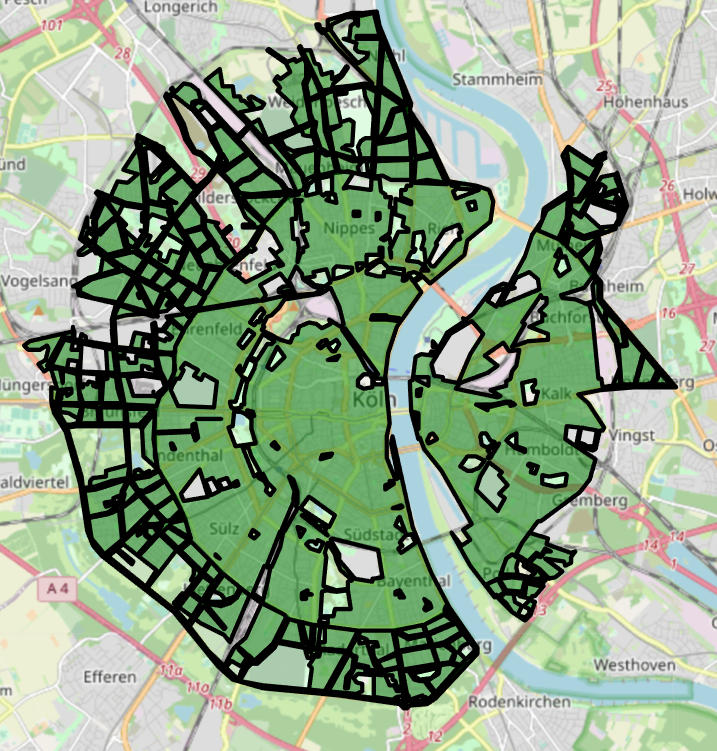
\includegraphics[width=0.50\textwidth]{Figures/discussion/flex_zones.png}
  \end{center}
  \caption{Next Bike's Flex Zones}
  \label{fig:flex_zones}
\end{figure}

Figure \ref{fig:problematic_hexagons} shows hexagons that are valid in terms of the 15-minute city by walking in green, those that are valid only by the addition of any sustainable mode of travel in yellow, and those that are not valid through any sustainable mode of travel in red.
We suspect that the very noticeable yellow ring around the city center is in an area where there are fewer POIs, but still a high availability of bicycles, that can compensate this sparsity.
This spatially shows where sustainable modes of travel are important to compensate for the sparsity of POIs.
These areas don't provide a close enough proximity to be considered valid in terms of the 15-minute city by walking alone.
However, with bicycle sharing and public transport they are.
In Figure \ref{fig:fixable_hexagons} we see that most of the hexagon in the ring are orange or green, which means that they are either fixable by bicycle sharing or by either bicycle sharing or public transport.
This again underlines that bicycle sharing is more effective, if it is present, than public transport (I\ref{item:bicycle_where_available}\&I\ref{item:bicycle_improves_accessibility}).
In the same figure, we can see that yellow hexagons, those that are only fixable through public transport, tend to exist in the regions that are more far away.
Also, the unfixable regions, marked in red,  mostly don't have bicycles near them, but they often have public transport nearby.
This suggests that bicycles are more effective than public transport to help a region become sub 15-minute (I\ref{item:bicycle_where_available}\&I\ref{item:bicycle_improves_accessibility}).

% pt only better at 90% pareto front
Investigating the cost and X-minute city metric Pareto fronts in Figures \ref{fig:mean_time_per_cost} and \ref{fig:quantile_time_per_cost}, as well as, the corresponding steps in Tables \ref{tab:differences_in_mean_pareto_front}, \ref{tab:differences_in_75_quantile_pareto_front} and \ref{tab:differences_in_90_quantile_pareto_front} shows that using a bicycle for 15 minutes always yields larger time gains than public transport except for the 10\% worst accessible hexagons (I\ref{item:bicycle_improves_accessibility} \& I\ref{item:pt_costlier_than_bicycle_sharing}).
This is a clear indicator for the superiority of bicycle sharing over public transport in terms of accessibility improvements, especially, when considering that the bicycle sharing infrastructure does not cover all of the considered area.

% cost stuff
Table \ref{tab:required_cost} and Figure \ref{fig:maximum_required_cost_for_x_minute_city} shows that bicycle sharing never costs more than public transport, if both are used (\ref{item:bicycle_more_cost_efficient_than_pt}).
We can also deduct this from the price of both and the fact that bicycles are never used more than 15 minutes.
We now that bicycles are never used for more than 15 minutes as the maximum cost, as seen in Table \ref{tab:required_cost} is \euro{1}, which is the price for a 15-minute ride.
Meanwhile, the shortest possible public transport trip costs \euro{2.20}, therefore as soon as public transport is used it always costs more than bicycles.
Nevertheless, this already shows that bicycle sharing is cheaper than public transport. 

In addition, knowing that bicycles never are used for more than 15 minutes tells us that at any location where bicycles are available, Cologne is a 15-minute city.
This is a strong indicator that bicycle sharing is able to make regions 15-minute city regions and therefore improves accessibility (I\ref{item:bicycle_improves_accessibility}).

Table \ref{tab:differences_in_mean_pareto_front} shows the average improvements of the X-minute city metric, at the steps in the Pareto front.
We see that bicycle sharing is on average more than 3 times more cost-efficient than public transport (I\ref{item:pt_costlier_than_bicycle_sharing}).
Further, investigating the differences at the 75\% and 90\% quantile Pareto fronts in Table \ref{tab:differences_in_75_quantile_pareto_front} and \ref{tab:differences_in_90_quantile_pareto_front}, shows that bicycle sharing always is more cost-efficient than public transport.

When looking at Table \ref{table:hexagons_with_walking_time_above_15_minutes} we see that bicycle sharing is able to make 13\% of hexagons that are not valid in terms of the 15-minute city by walking alone, valid, which is more than public transport.
% This shows that bicycle sharing is more effective than public transport (\ref{item:bicycle_improves_accessibility}).

Looking at the spatial distribution of those hexagons in Figure \ref{fig:fixable_hexagons}, we see that the orange hexagons, which are those that, become valid in terms of the 15-minute city only through bicycle sharing, are mostly located at the city's border, where the "Flex-Zone" is still active.
This again shows that the effectiveness of  bicycle sharing highly depends on the flex zone (\ref{item:bicycle_where_available}).


%END

% not sure where to put this
% Another difference between bicycles and public transport is that they differ notably in their speed and route flexibility. 
% Public transport typically travels faster than bicycles, which offers a clear advantage for covering long distances. 
% This speed is particularly beneficial when some POIs are far away, as public transport can effectively bridge these larger gaps. 
% However, the fixed routes of public transport mean that users may not always disembark close to their desired POI. 
% In contrast, bicycles offer the flexibility of route choice, allowing users to tailor their journey to arrive nearer to the POI. 
% This also aligns with the finding that public transport tends to be most effective for the least accessible hexagons, where distance to POIs is a significant factor.

% end


\subsubsection{Bicycle Sharing and Public Transport - Substitutes or Complements?}
% introduction of substitutional effects and complement I & II
As already mentioned we found clear evidence that bicycle sharing and public transport have a positive effect on accessibility according to the X-minute city metric.
It is, however, not clear whether these modes are substitutional to each other, meaning that one mode is able to compensate the other, or whether they are complements.
We potentially could observe two sorts of complementary effects.
\begin{itemize}
  \renewcommand{\labelenumi}{Complement \theenumi.}
  \item Bicycle sharing and public transport are effective under different circumstances and in different areas \label{item:different_circumstances}
  \item bicycle sharing and public transport used together is necessary to improve accessibility \label{item:used_together}
\end{itemize}
The presence of complement \ref{item:different_circumstances} means that one mode cannot replace the other, and each is necessary under specific circumstances.
The presence of complement \ref{item:used_together} means that both modes need to be used together in a single journey in order to achieve the highest accessibility.
Both effects can be described as complementary effects, and they are not mutually exclusive, which means that we can potentially observe both.

In our results we find evidence for both effects, yet complement \ref{item:different_circumstances} is more pronounced.
We will now reiterate our results and show how they support the complements above.

Table \ref{tab:optimal_x_minute_city_metric} shows that the combined scenario on average yields better accessibility than bicycle sharing and public transport alone.
This suggests that either complement I or complement II must be present.

% complement I
We see evidence for complement I in the observation that bicycle sharing is most effective for the 80\% more accessible hexagons, while public transport is mostly only effective for the 20\% least accessible hexagons.

Table \ref{table:hexagons_with_walking_time_above_15_minutes} shows how many hexagons in which people are not able to reach all necessities in 15 minutes by walking can reach all necessities in under 15 minute by public transport or bicycle sharing.
We see that bicycles sharing, and public transport alone are roughly of equal importance, as they fix 13\% and 11\% of hexagons, respectively.
In addition, a lot more hexagons are fixed by only one of them (24\%) than by either of them (7\%).
This again suggests that complement I is present.


Table \ref{table:hexagons_with_walking_time_above_15_minutes} also shows that the combined scenario only fixes around 2\% and is therefore not very impactful.
Nevertheless, we prove that the effect of complement II is present.

% implications
The presence of complement I should make us aware that the effectiveness of either mode is highly dependent on the spatial circumstances of the region.
Some regions might benefit more from bicycle sharing, while others benefit more from public transport.
It is therefore, necessary to analyze each region separately, to maximize the positive effect of sustainable modes of travel.
% implications END
%END

% not sure where to put this "conclusion"
% Our findings lead to the conclusion that enhancing bicycle availability in areas with low accessibility could yield significant benefits.
% Additionally, the observed dynamics suggest that bicycles are more advantageous in areas with low to medium accessibility, while public transport predominantly benefits the least accessible areas.
% This again indicates that bicycles and public transport serve complementary, rather than substitutable, roles in urban mobility networks.
% Therefore, removing one mode of transportation cannot be effectively compensated for by simply increasing the other, as each serves distinct and crucial functions in addressing different aspects of urban accessibility.




\subsubsection{Monetary Considerations}

Table \ref{tab:differences_in_mean_pareto_front} shows how a minute of saved time costs for cycling and public transport, respectively.
The most cost-efficient variant, bicycle sharing, enables users to save 1.68 minutes per euro, which might not be worth it for most people.
The 1.68 minutes per euro spent, in other words means that to save a minute of time people have to spend around 62 cents.
Comparing this to the minimum wage in Germany of 12 euro per hour in 2022 \shortcite{federalstatisticalofficegermanyMinimumWages}, which is 20 cents per minute, shows that it takes around three minutes to make enough money to save one minute, which obviously is not worth it.
This means that currently on average the sustainable modes of travel are too expensive.

Even when looking at the least accessible regions (90\% quantile) separately in Figure \ref{fig:90_quantile_time_per_cost}, where we have the largest improvement possible, the most cost-efficient mode of transport, which is bicycle, only yields an improvement of two minutes per euro, which again does not result in a net positive for people who earn the minimum wage.


With the help of the monthly cost depicted in in Table \ref{tab:monthly_costs_per_scenario_15} and \ref{tab:monthly_costs_per_scenario_10} we are able to derive recommendations for the price of a monthly ticket or subscription that is appealing to residents, that have to use public transport or bicycle sharing in order to reach certain amenities in under 10 or 15 minutes.
We expect that such a monthly ticket would reduce the cost the trips necessary to reach the ameneties to zero.
In our experiment in the city of Cologne, this is plausible, as the public transport tickets indeed allow for unlimited travel within the city, while NextBike's subscription makes trips that are under 30 minutes free.

Looking at the Tables we note that the monthly cost for the combined scenario and the bicycle scenario are the same, which shows that in the combined scenario only bicycle sharing is used.
In the 15-minute benchmark, we see that in order to appeal to at least 50\% of the population, a public transport ticket should cost less than \euro{8.80}, while a bicycle sharing subscription should cost less than \euro{4}.
In the 10-minute benchmark we see a similar pattern: the median cost for the bicycle and combined scenario is \euro{9}, while the median cost for the public transport scenario is \euro{19.80}.
Currently, a NextBike subscription costs \euro{10} per month, while the most common public transport ticket, the "Deutschlandticket", costs \euro{49} per month.
Both of these prices are significantly higher than the median cost for the bicycle and combined scenario, which means that a monthly ticket is not worth it for most people.

Table \ref{tab:monthly_costs_for_cars} shows the monthly cost for cars, excluding acquisition costs.
With the difference between monthly car cost and the monthly cost of the bicycle, combined and public transport scenario, we can calculate how large acquisition costs for a car can be, so that it is still cheaper than the sustainable modes of travel.
In the case of the 15-minute benchmark the average car costs are \euro{1.69}, while the average cost for the bicycle and combined scenario are \euro{5.79}, resulting in a difference of \euro{4.10} per month or \euro{49.20} per year.
This difference compared to the usual acquisition cost of a car is so low, that it is not monetarily worth it to buy a car, if the same journey can be made with bicycle sharing or public transport.
In addition, we have to keep in mind that our estimates for the speed of cars are very optimistic, as we assume that there is no traffic and that parking is always available.
Obviously, we can only state this for areas in which the accessibility using sustainable modes of travel suffices.
From table \ref{table:hexagons_with_walking_time_above_15_minutes} we know that 67\% of hexagons in which walking alone is not sufficient, only cars are able to make all amenities accessible in under 15 minutes.



\subsubsection{Uncertainty}

The standard deviation of the average time it takes to reach all necessities for bicycles is 1 minute and 10 second. 
Relating this to the improvement compared to walking of 1 minute and 38 seconds, we see that the uncertainty is quite large.
This shows us that the placement of bicycles significantly impacts the effectiveness of the bicycle sharing scenario (I\ref{item:bicycle_where_available}).

It is interesting to note that bicycles suffer more from uncertainty than public transport, as public transport only has a standard deviation of 16 seconds.
Relating the standard deviation to the improvement compared to walking of 1 minute and 28 seconds, it is by far not as impactful as with bicycles.
However, the standard deviation strongly depends on the choices of our sub-scenarios. 
For public transport we tried 08:00, 12:00 and 18:00.
We suspect that the variance for public transport would increase more drastically and eventually surpass the one of bicycle sharing if we choose more unusual times like midnight.
In addition, the schedule of public transport is often the same for full hours.
We could get a more realistic picture, if we would add more times with non-zero minutes to our sub scenarios.

We should also note that the comparison of variances should be taken with caution as the method for selecting the sub-scenarios differ per scenario.
For bicycle sharing we employed a clustering method, while for public transport we made a qualitative choice. 

% \subsubsection{Potential of Sustainable Modes To Transform Cities To 15-Minute Cities}
%
% copied to implications
% We know that approximately 69\% of all considered hexagons and with that 69\% of all residential in the administrative district Cologne ("Stadtkreis Köln") are 15-minute city by walking, which shows us that Cologne largely already has an excellent accessibility.

% Table \ref{table:hexagons_with_walking_time_above_15_minutes} shows that a majority (67\%) of the hexagons that are currently not 15-minute city regions are not fixed by any of the sustainable modes of travel, which shows that the impact of public transport and bicycle is limited.
% Nevertheless, the impact of bicycle and public transport on making regions valid in terms of the 15-minute city is not negligible, as those modes of transport still achieve to fix 33\% of hexagons that are not yet valid in terms of the 15-minute city by walking alone.

% copied to "effectiveness of bicycle sharing"
% Figure \ref{fig:problematic_hexagons} shows hexagons that are valid in terms of the 15-minute city by walking in green, those that are valid only by the addition of any sustainable mode of travel in yellow, and those that are not valid through any sustainable mode of travel in red.
% We suspect that the very noticeable yellow ring around the city center is in an area where there are fewer POIs, but still a high availability of bicycles, that can compensate this sparsity.
% This spatially shows where sustainable modes of travel are important to compensate for the sparsity of POIs.
% These areas don't provide a close enough proximity to be considered valid in terms of the 15-minute city by walking alone.
% However, with bicycle sharing and public transport they are.
% In Figure \ref{fig:fixable_hexagons} we see that most of the hexagon in the ring are orange or green, which means that they are either fixable by bicycle sharing or by either bicycle sharing or public transport.
% This again underlines that bicycle sharing is more effective, if it is present, than public transport.
% In the same figure, we can see that yellow hexagons, those that are only fixable through public transport, tend to exist in the regions that are more far away.

% copied to "effectiveness of bicycle sharing"
% The unfixable regions mostly don't have bicycles near them, but they often have public transport nearby.
% This suggests that bicycles are more effective than public transport to help a region become sub 15-minute.

\subsection{Implications}
\label{sec:implications}

From our interpretation of the results, we can derive several implications for the city of Cologne and for accessibility in cities in general.
We will structure our implications into two sections, first we will discuss what already works well, and then we will discuss measures that can be taken to improve accessibility.

% what works well
What already works well is the improvement of accessibility through public transport in remote areas.
As long as there are areas with low accessibility, that is caused by a low availability of POIs, public transport will be an effective measure.
Also bicycle sharing is able to improve the accessibility everywhere, where there are bicycles available.
For the most part, at least for Cologne, this means that bicycle sharing is highly effective where the "Flez-Zone" is located.
It is important to understand the relation between its effectiveness and the location of this zone.
As most of Cologne's central parts are covered by the zone, we already observe it's massive positive effects on accessibility.
In addition, approximately 69\% of all considered hexagons and with that 69\% of all residential in the administrative district Cologne ("Stadtkreis Köln") are 15-minute city by walking, which shows us that Cologne largely already has an excellent accessibility.
Interestingly, this \shortciteA{nicolettiDisadvantagedCommunitiesHave2023} calculated a vastly higher number. 

% improvements
% improvement 1: turning more non-15 minute regions into 15-minute regions
The observation that approximately 31\% of Cologne's area lacks access to essential services within a 15-minute walk highlights the potential for improvements.
We hypothesized that the introduction of bicycle sharing and enhanced public transport could significantly reduce these areas by improving accessibility.
However, as indicated in Table \ref{table:hexagons_with_walking_time_above_15_minutes}, a majority (67\%) of the hexagons currently not meeting 15-minute city criteria remain to not meet the criteria even with these sustainable modes.
Yet, it is important to note the impact of bicycles and public transport in converting 33\% of these hexagons into areas meeting the 15-minute city criteria.
To further amplify their effectiveness, we propose two strategies.
Firstly, expanding the 'flex zone' areas where bicycles are available, into regions with currently poor accessibility. 
Given the observed correlation between bicycle availability and enhanced accessibility, this approach will very likely yield substantial improvements.
Secondly, we recommend establishing high-frequency public transport lines to connect to remote, low-accessible areas. 
Our findings suggest that public transport effectively improves accessibility in these regions. 
However, considering the potential impracticality of extending the flex zone to these distant areas, adding or enhancing public transport routes could be a more feasible solution.

% improvement 2: effectively managing the bicycle sharing fleet
We have demonstrated that the success of a bicycle-sharing is closely tied to the availability of bicycles.
This availability primarily hinges on two factors: the location of the 'flex zone' and the manner in which bicycles are distributed within it.
Significantly, our findings reveal that the effectiveness of the program varies greatly across different sub-scenarios, highlighting the importance of strategic bicycle distribution.
Therefore, the careful management of bicycle placement and timely relocations are crucial for the system's efficiency.
To optimize the effectiveness of bicycle sharing, it is essential to conduct regular analyses of system demand and adjust bicycle distribution in response to these insights.
\shortciteA{heRobustRepositioningVehicle2020,luOptimizingProfitabilityQuality2018b,benjaafarDynamicInventoryRepositioning2018a} have already done research in how to effectively relocate bicycles.

% TODO:
% improvement 3: reducing costs


% don't know what to do with this
% Merkenich & rhine bridge
% In Figure \ref{fig:optimal_map} we observed that Merkenich, which is located at the other side of the Rhine next to Leverkusen, is one of the least accessible regions in Cologne.
% From Figure ???, we now that there are plenty of POIs for all categories in Leverkusen, which are very close to the problematic region.
% This indicates a lack of mobility crossing the Rhine river.
% As a bridge is already existing, we suggest providing a frequent public transport line to improve the accessibility in Merkenich.

\subsection{Limitations}
\label{sec:limitations}

% This section shoes the constraints and boundaries within which our current study on bicycle-sharing programs and urban accessibility operates.

% Exclusion of Traffic and Parking Factors

A significant limitation of our analysis is the omission of traffic conditions and parking availability. 
Urban traffic dynamics can significantly influence the practicality and speed of bicycle and especially car travel, potentially skewing the perceived efficiency.
Similarly, the availability of parking, plays a crucial role in urban mobility, particularly in cities.
By not accounting for these factors, our study may not fully capture the complexities and challenges faced by urban commuters, possibly overestimating the effectiveness of bicycle-sharing and car travel in congested urban environments.

Another critical limitation is the exclusion of reliability issues such as public transport outages or traffic disruptions due to accidents. 
These events can drastically affect transportation dynamics in a city. 
For instance, a public transport outage might temporarily increase the demand for bicycles, while an accident could impede bicycle routes. 
Not considering these variables limits the scope of our study, particularly in understanding the resilience and adaptability of bicycle-sharing and public transport systems.

The usefulness of the X-minute-city metric employed in our study, which assesses accessibility based on the ability to reach any POI that is assigned to a category should be taken with caution as well.
For example, the access to a pet doctor, which is a health POI, is considered equivalent to the access to a hospital.
While this metric provides a quantifiable measure of accessibility, it may not comprehensively represent the diverse needs of an urban population. 

Our analysis also reveals a limitation concerning the scalability of transport modes. 
While bicycles significantly improve the X-minute city metric in our study, suggesting enhanced accessibility, they inherently lack the scalability of public transport. 
A bicycle may offer a convenient solution for an individual, but it does not address the mass transit needs of a larger population. 
This aspect is particularly crucial in dense urban areas where public transport systems are more efficient in moving large numbers of people. 
Therefore, while bicycles contribute to urban accessibility, they should be considered part of a broader, multi-modal transport strategy rather than a standalone solution.

% limitations conclusion
% In conclusion, while our study sheds light on the potential of bicycle-sharing and public transport systems in enhancing urban accessibility, it is important to consider these limitations. 
% The exclusion of factors such as traffic dynamics, parking availability, and reliability issues, along with the limitations of the chosen metric and the scalability of bicycles, suggest areas for further research. 
% Acknowledging these limitations helps in framing our findings within a realistic urban context and underscores the need for comprehensive, multi-faceted approaches in urban planning and transportation studies.

\subsection{Future Work}
\label{sec:future_work}

Building upon the findings of our current study, it is essential to explore new avenues to deepen our understanding of urban mobility and enhance bicycle-sharing systems. 
This section outlines potential directions for future research that can contribute significantly to this field.

% Investigating Public Transport Disruptions
A crucial area of future research is examining the impact of public transport disruptions on accessibility.
Disruptions such as strikes, maintenance, or accidents can drastically alter commuting patterns. 
Investigating these scenarios could involve comparing accessibility between normal and disrupted conditions to determine the impact of outages and to what extend bicycle sharing or other modes can compensate these outages.
This research can provide valuable insights into the role of bicycle-sharing as an alternative mode of transport during public transport failures.

% Flex Zone Enhancements
Another promising research direction is to study the effects of modifications to the flex zone. 
Changing the area where bikes can be borrowed and returned may significantly influence the accessibility improvements caused by bike-sharing. 
Future studies could experiment with different sizes and placements of flex zones to determine optimal configurations that maximize accessibility and efficiency.
These research endeavors should consider or even incorporate the dynamics of bicycle relocations.

% Improving Public Transport Lines
Investigating the impact of adding new or improving existing public transport lines on bicycle-sharing systems presents another research opportunity. 
Such a study could explore how enhancements in public transport affect the accessibility in currently inaccessible areas.
Understanding these dynamics is crucial for integrated urban transport planning that caters to diverse commuter needs.

% Comprehensive Analysis of Transportation Usage
A comprehensive study on the usage patterns of roads, bicycles, and public transport is also essential. 
With the help of our current study, it is possible to find the paths that people would take if they would try to get from a specific point to another specific point.
Using this together with realistic demand data, yields in a set of paths, that can be analyzed to find potential bottlenecks.
The results could inform urban planning and policy decisions, leading to more efficient and responsive urban transport systems.

% Conclusion of Future Research Ideas
% To conclude, the proposed research directions offer exciting possibilities for advancing our understanding of urban transportation systems. By investigating the impact of public transport disruptions, exploring flex zone enhancements, analyzing the effects of improvements in public transport lines, and conducting a comprehensive analysis of transportation usage, future studies can significantly contribute to the development of more efficient, accessible, and resilient urban mobility solutions. These research endeavors will not only build on the foundations laid by our current study but also pave the way for innovative approaches to tackling the challenges of urban transportation.






%%%%%%%%%%%%%%%%%%%%%%%%%%%%%%%%%%%%%%%%%%%%%%%%%%%%%%%%%%%%%
%APPENDICES
%%%%%%%%%%%%%%%%%%%%%%%%%%%%%%%%%%%%%%%%%%%%%%%%%%%%%%%%%%%%%


\appendix
\renewcommand*{\thesection}{\Alph{section}}\textbf{}

% APPENDIX A
\clearpage
\section{Appendix - Overpass Query for Boundary of Cologne}
\label{app:overpass_query}
\begin{verbatim}
[out:json][timeout:50];
area["name"="Köln"]->.searchArea;
relation["boundary"="administrative"]["admin_level"="6"](area.searchArea);
out body;
>;
out skel qt;
\end{verbatim}

\section{Appendix - Pyrosm Network Filter}
\label{app:pyrosm_network_filter}

Pyrosm filters out all ways that have the following tags:

\begin{table}[h]
\centering
\caption{Driving Filter}
\begin{tabular}{|c|p{10cm}|}
\hline
\textbf{Key}         & \textbf{Values}                                                                                                             \\ \hline
area                 & yes                                                                                                                         \\ \hline
highway              & cycleway, footway, path, pedestrian, steps, track, corridor, elevator, escalator, proposed, construction, bridleway, abandoned, platform, raceway \\ \hline
motor\_vehicle       & no                                                                                                                          \\ \hline
motorcar             & no                                                                                                                          \\ \hline
service              & parking, parking\_aisle, private, emergency\_access                                                                         \\ \hline
\end{tabular}
\end{table}


\begin{table}[h]
\centering
\caption{Walking Filter}
\begin{tabular}{|c|p{10cm}|}
\hline
\textbf{Key}         & \textbf{Values}                                                                                                             \\ \hline
area                 & yes                                                                                                                         \\ \hline
highway              & cycleway, motor, proposed, construction, abandoned, platform, raceway, motorway, motorway\_link                             \\ \hline
foot                 & no                                                                                                                          \\ \hline
service              & private                                                                                                                     \\ \hline
\end{tabular}
\end{table}


\begin{table}[h]
\centering
\caption{Cycling Filter}
\begin{tabular}{|c|p{10cm}|}
\hline
\textbf{Key}         & \textbf{Values}                                                                                                             \\ \hline
area                 & yes                                                                                                                         \\ \hline
highway              & footway, steps, corridor, elevator, escalator, motor, proposed, construction, abandoned, platform, raceway, motorway, motorway\_link \\ \hline
bicycle              & no                                                                                                                          \\ \hline
service              & private                                                                                                                     \\ \hline
\end{tabular}
\end{table}


\section{Appendix - Categories and Their Corresponding OSM Tags}
\label{app:categories_and_osm_tags}

\begin{table}[ht]
\centering
\caption{Categories and Their Corresponding OSM Tags}
\label{tab:categories}
\footnotesize
\begin{tabular}{|l|l|p{10cm}|}
\hline
\textbf{Category} & \textbf{OSM Key} & \textbf{OSM Value} \\ \hline
Grocery           & shop             & alcohol, bakery, beverages, brewing supplies, butcher, cheese, chocolate, coffee, confectionery, convenience, deli, dairy, farm, frozen food, greengrocer, health food, ice-cream, pasta, pastry, seafood, spices, tea, water, supermarket, department store, general, kiosk, mall \\ \hline
Education         & amenity          & college, driving school, kindergarten, language school, music school, school, university \\ \hline
Health            & amenity          & clinic, dentist, doctors, hospital, nursing home, pharmacy, social facility \\ \hline
Banks             & amenity          & atm, bank, bureau de change, post office \\ \hline
Parks             & leisure          & park, dog park \\ \hline
Sustenance        & amenity          & restaurant, pub, bar, cafe, fast-food, food court, ice-cream, biergarten \\ \hline
Shops             & shop             & department store, general, kiosk, mall, wholesale, baby goods, bag, boutique, clothes, fabric, fashion accessories, jewelry, leather, watches, wool, charity, secondhand, variety store, beauty, chemist, cosmetics, erotic, hairdresser, hairdresser supply, hearing aids, herbalist, massage, medical supply, nutrition supplements, optician, perfumery, tattoo, agrarian, appliance, bathroom furnishing, do-it-yourself, electrical, energy, fireplace, florist, garden centre, garden furniture, fuel, glaziery, groundskeeping, hardware, houseware, locksmith, paint, security, trade, antiques, bed, candles, carpet, curtain, flooring, furniture, household linen, interior decoration, kitchen, lighting, tiles, window blind, computer, electronics, hifi, mobile phone, radio-technics, vacuum cleaner, bicycle, boat, car, car repair, car parts, caravan, fishing, golf, hunting, jet ski, military surplus, motorcycle, outdoor, scuba diving, ski, snowmobile, swimming pool, trailer, tyres, art, collector, craft, frame, games, model, music, musical instrument, photo, camera, trophy, video, videogames, anime, books, gift, lottery, newsagent, stationery, ticket, bookmaker, cannabis, copy shop, dry cleaning, e-cigarette, funeral directors, laundry, moneylender, party, pawnbroker, pet, pet grooming, pest control, pyrotechnics, religion, storage rental, tobacco, toys, travel agency, vacant, weapons, outpost \\ \hline
\end{tabular}
\normalsize
\end{table}

\section{Appendix - Experiment Module Matrix Configuration}
\label{app:experiment_module_matrix_configuration}

% walking step
    % initial_steps = [[walking_step]]
    % repeating_steps = []

\begin{figure}[ht]
    \centering
    \begin{subfigure}{0.45\linewidth}
        \centering
        \[
        \begin{pmatrix}
            \text{walking module} \\
        \end{pmatrix}
        \]
        \caption{Initial Matrix}
    \end{subfigure}
    \hfill
    \begin{subfigure}{0.45\linewidth}
        \centering
        \[
        \begin{pmatrix}
            \\
        \end{pmatrix}
        \]
        \caption{Repeating Matrix}
    \end{subfigure}
    \caption{Walking Scenario Module Matrices}
    \label{fig:walking_scenario_module_matrix}
\end{figure}

% combined mode 
    % initial_steps = [[walking_step]]
    % repeating_steps = [
    %     [bicycle_step, public_transport_step],
    %     [walking_step],
    % ]

\begin{figure}[ht]
    \centering
    \begin{subfigure}{0.45\linewidth}
        \centering
        \[
        \begin{pmatrix}
            \text{walking module} \\
        \end{pmatrix}
        \]
        \caption{Initial Matrix}
    \end{subfigure}
    \hfill
    \begin{subfigure}{0.45\linewidth}
        \centering
        \[
        \begin{pmatrix}
            \text{free-floating vehicle} & \text{public transport} \\
            \text{sharing module} & \text{module} \\
            \\
            \text{walking module} & \\
        \end{pmatrix}
        \]
        \caption{Repeating Matrix}
    \end{subfigure}
    \caption{Combined scenario module matrices}
    \label{fig:combined_scenario_module_matrix}
\end{figure}

% personal car
    % initial_steps = []
    % repeating_steps = [[car_step]]


\begin{figure}[ht]
    \centering
    \begin{subfigure}{0.45\linewidth}
        \centering
        \[
        \begin{pmatrix}
            \\
        \end{pmatrix}
        \]
        \caption{Initial Matrix}
    \end{subfigure}
    \hfill
    \begin{subfigure}{0.45\linewidth}
        \centering
        \[
        \begin{pmatrix}
            \text{personal car module}\\
        \end{pmatrix}
        \]
        \caption{Repeating Matrix}
    \end{subfigure}
    \caption{Personal Car Scenario Module Matrices}
    \label{fig:personal_car_scenario_module_matrix}
\end{figure}

% bicycle only
    % initial_steps = [[walking_step]]
    % repeating_steps = [
    %     [bicycle_step],
    %     [walking_step],
    % ]


\begin{figure}[ht]
    \centering
    \begin{subfigure}{0.45\linewidth}
        \centering
        \[
        \begin{pmatrix}
            \text{walking module} \\
        \end{pmatrix}
        \]
        \caption{Initial Matrix}
    \end{subfigure}
    \hfill
    \begin{subfigure}{0.45\linewidth}
        \centering
        \[
        \begin{pmatrix}
            \text{public transport module} \\
            \text{walking module} \\
        \end{pmatrix}
        \]
        \caption{Repeating Matrix}
    \end{subfigure}
    \caption{Public Transport Scenario Module Matrices}
    \label{fig:public_transport_scenario_module_matrix}
\end{figure}

% public transport only
    % initial_steps = [[walking_step]]
    % repeating_steps = [[public_transport_step], [walking_step]]

\begin{figure}[ht]
    \centering
    \begin{subfigure}{0.45\linewidth}
        \centering
        \[
        \begin{pmatrix}
            \text{walking module} \\
        \end{pmatrix}
        \]
        \caption{Initial Matrix}
    \end{subfigure}
    \hfill
    \begin{subfigure}{0.45\linewidth}
        \centering
        \[
        \begin{pmatrix}
            \text{free-floating vehicle sharing module} \\
            \text{walking module} \\
        \end{pmatrix}
        \]
        \caption{Repeating Matrix}
    \end{subfigure}
    \caption{Bicycle Scenario Module Matrices}
    \label{fig:bicycle_scenario_module_matrix}
\end{figure}


\section{Appendix - Monthly Visits per Category}
\label{app:monthly_visits_per_category}

\paragraph{Grocery}
3 times per week according to \shortciteA{nilssonWhoShopsGroceries2015}.
Resulting in approximately 12 times per month.

\paragraph{Education}
5 times per week, as we assume that students visit their school or university 5 times per week.

\paragraph{Health}
5.09 per year according to \shortciteA{eurostatHowOftenYou2019}.
Resulting in approximately 0.42 times per month.

\paragraph{Banks}
9 per month according to \shortciteA{optconnectATMStatistics}.

\paragraph{Parks}
29 per year according to \shortciteA{nationalrecreationandparkassociationNumberTimesAmericans2016}.
Resulting in approximately 2.42 times per month.

\paragraph{Sustenance}
6.12 per month according to \shortciteA{saprykinImpactSocialMedia2016}.

\paragraph{Shops}
4 per month according to \shortciteA{businessplusHowOftenPeople2019}.






%%%%%%%%%%%%%%%%%%%%%%%%%%%%%%%%%%%%%%%%%%%%%%%%%%%%%%%%%%%%%
%BIBLIOGRAPHY
%%%%%%%%%%%%%%%%%%%%%%%%%%%%%%%%%%%%%%%%%%%%%%%%%%%%%%%%%%%%%

\clearpage
\renewcommand*{\thesection}{}\textbf{}

\bibliographystyle{apacite}
\bibliography{Bibliography.bib}


\end{document}
